% Load the kaobook class
\documentclass[
	fontsize=10pt, % Base font size
	twoside=true, % Use different layouts for even and odd pages (in particular, if twoside=true, the margin column will be always on the outside)
	%open=any, % If twoside=true, uncomment this to force new chapters to start on any page, not only on right (odd) pages
%%	secnumdepth=1, % How deep to number headings. Defaults to 1 (sections)
]{kaobook}

\newcommand{\discipline}{Sciences Industrielles de l'Ingénieur -- PSI$\star$}
\newcommand{\auteur}{Xavier Pessoles}
\newcommand{\repRel}{../..}

\input{\repRel/Style/packages_v2}
\newcommand{\repStyle}{\repRel/Style}
\input{\repRel/Style/macros_SII_v2}
\input{\repRel/Style/environment_v2}
\usepackage{\repStyle/UPSTI_pedagogique}


% Choose the language
\frenchsetup{StandardItemLabels=true}



% Load the bibliography package
\usepackage{kaobiblio}
%\addbibresource{Cy_01_ModelisationSystemes.bib} % Bibliography file

% Load mathematical packages for theorems and related environments
\usepackage{kaotheorems}

% Load the package for hyperreferences
\usepackage{kaorefs}

\graphicspath{{images/}{./}} % Paths where images are looked for

\makeindex[columns=3, title=Alphabetical Index, intoc] % Make LaTeX produce the files required to compile the index


\begin{document}

%%----------------------------------------------------------------------------------------
%%	BOOK INFORMATION
%%----------------------------------------------------------------------------------------

%\titlehead{Document Template}
\title[SII en PSI*]{SII en PSI* -- Exercices d'application}
\author[XP]{Xavier Pessoles}
\date{\today}
%\publishers{An Awesome Publisher}

%----------------------------------------------------------------------------------------
%
\frontmatter % Denotes the start of the pre-document content, uses roman numerals
\maketitle

\begingroup % Local scope for the following commands
\tableofcontents
\endgroup

%%----------------------------------------------------------------------------------------
%%	MAIN BODY
%%----------------------------------------------------------------------------------------
%
\mainmatter % Denotes the start of the main document content, resets page numbering and uses arabic 

\setchapterstyle{kao}

\setcounter{margintocdepth}{\sectiontocdepth}
\marginlayout
\graphicspath{{\repStyle/png}}

\pagestyle{xp.scrheadings}


%%%%%
\newcommand{\repExo}{Application_01_ROV}
\newcommand{\nomExo}{Application_01_ROV}
%\newcounter{cptApplication}[chapter]
%\newcounter{cptTD}[chapter]
\AtBeginEnvironment{corrige}{\small}

\livrettrue % Livrettrue :  eleve sans les corrections
\collefalse
\normaltrue
%%%%%
\setcounter{cptApplication}{1}
\setcounter{cptTD}{1}
\newcommand{\exer}{\subsection*}
\newcommand{\td}{}

\setchapterpreamble[u]{\margintoc} 
\chapter{Évaluer les performances d'un SLCI} 
\section{Évaluer la stabilité en utilisant la BF, les pôles de la BF} 
\section{Évaluer la stabilité en utilisant les marges de la BO} 
\graphicspath{{\repStyle/png/}{../PERF/PERF-02-Marges/61_Hemostase/images/}} 
\normaltrue \difficilefalse \tdifficilefalse
\correctionfalse
%\UPSTIidClasse{11} % 11 sup, 12 spé
%\newcommand{\UPSTIidClasse}{11}

\exer{Hemostase -- Stabilité$\star$ \label{PERF:02:C2:03:stab:61}}

\setcounter{question}{0}\marginnote{\xpComp{PERF}{02}}%\index{Compétence C2-03}\index{Compétence PERF-02}
\index{Compétence C2-03}
\index{Schéma-blocs}
\index{Stabilité}

%%%%%%%%%%%%%%%%%%%%%%%%%%%%%%%


\ifprof
\else
La modélisation de l'asservissement de position est donnée par le schéma-bloc ci-dessous dans lequel $K_2 = 2,78 \cdot 10^{-2} \text{N}^{-1}$, $K_1 = \SI{856}{s^{-1}}$, $T_m= 3\cdot  10^{-2} s$.

Le couple résistant $C_r$ est constant et vaut $C_{r0} = 2,7 \cdot 10^{-3} \text{Nm}$.


\begin{marginfigure}
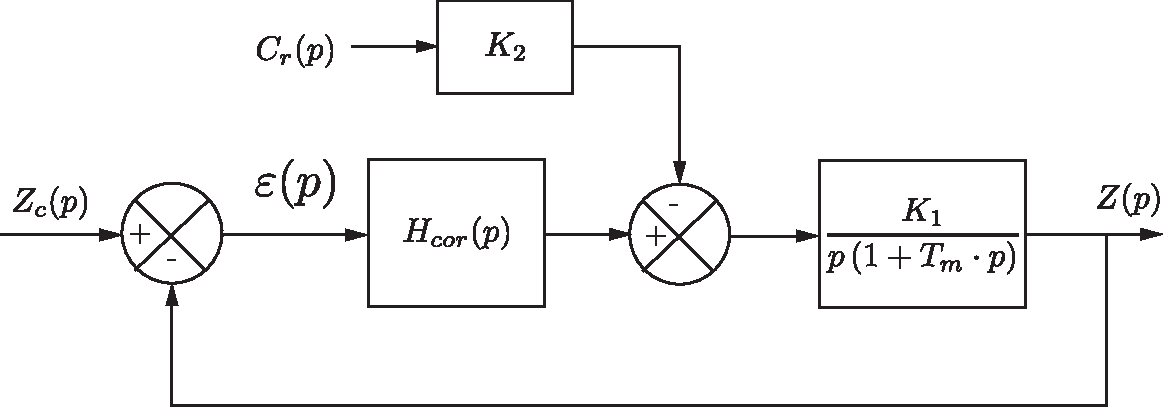
\includegraphics[width=\linewidth]{64_01.pdf}
\end{marginfigure}

On suppose le correcteur proportionnel : $H_{\text{cor}}(p)=K_p$.

Les performances du système sont détaillées dans le diagramme des exigences partiel.% (figure \ref{req}). 


\begin{marginfigure}
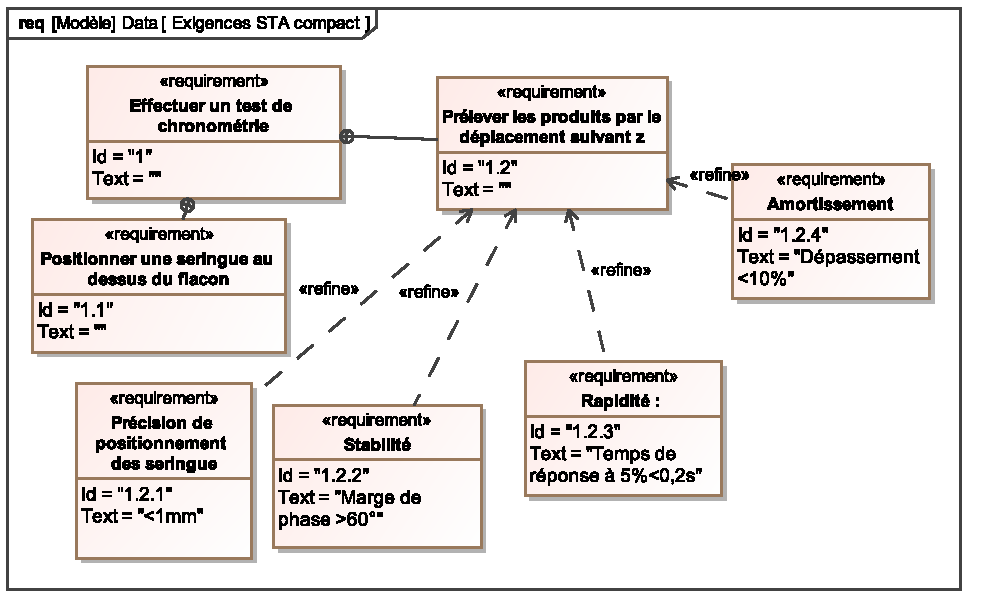
\includegraphics[width=\linewidth]{req.pdf}
\end{marginfigure}



\fi
\question{Déterminer l'expression de la fonction de transfert en boucle ouverte $H_{\text{bo}}(p)=\left(\frac{Z(p)}{\varepsilon(p)}\right)_{C_r(p)=0}$ ainsi que la fonction de transfert $H_{\text{cr}}(p)=\left(\frac{Z(p)}{C_r(p)}\right)_{Z_c=0}$.}
\ifprof
%\begin{corrige}~\\

$H_{\text{bo}}(p) = H_{\text{cor}}(p) \dfrac{K_1}{p\left(1+T_m p\right)}$ $=  \dfrac{K_1 K_p}{p\left(1+T_m p\right)}$.

$H_{\text{cr}}(p)= -K_2\dfrac{\dfrac{K_1}{p\left(1+T_m p\right)}}{1+H_{\text{cor}}(p) \dfrac{K_1}{p\left(1+T_m p\right)}}$

$= -K_2\dfrac{K_1}{p\left(1+T_m p\right)+H_{\text{cor}}(p) K_1}$
$= -\dfrac{K_1K_2}{p\left(1+T_m p\right)+K_p K_1}$
%\end{corrige}
\else
\fi

\question{Déterminer l'erreur statique pour une entrée de type échelon d'amplitude $Z_{c0}$ dans l'hypothèse d'une perturbation nulle ($C_{r0}$). Déterminer ensuite l'erreur due à une perturbation constante $C_{r0}$, dans le cas d'une
consigne de position nulle ($Z_c=0$). En déduire la valeur de $K_p$ pour satisfaire le critère de précision du cahier des charges.}
\ifprof
%\begin{corrige}
Exprimons $\varepsilon(p)$ en fonction de $Z_c(p)$ et $C_{r}(p)$ :

$
\varepsilon(p)=Z_c(p)-Z(p) = Z_c(p)- \left(\varepsilon(p) H_{\text{cor}}(p)-   K_2 C_r(p)\right) \dfrac{K_1}{p\left(1+T_m p\right)}$

$\Leftrightarrow \varepsilon(p)\left(1 +  H_{\text{cor}}(p)\dfrac{K_1}{p\left(1+T_m p\right)} \right) 
= Z_c(p) + K_2 C_r(p) \dfrac{K_1}{p\left(1+T_m p\right)}$

$\Leftrightarrow \varepsilon(p)  = 
Z_c(p)\dfrac{1}{1 +  H_{\text{cor}}(p)\dfrac{K_1}{p\left(1+T_m p\right)}} 
+   K_2 C_r(p) \dfrac{K_1}{p\left(1+T_m p\right)} \dfrac{1}{1 +  H_{\text{cor}}(p)\dfrac{K_1}{p\left(1+T_m p\right)}}$

$\Leftrightarrow \varepsilon(p)  = 
Z_c(p)\dfrac{{p\left(1+T_m p\right)}}{{p\left(1+T_m p\right)} +  H_{\text{cor}}(p){K_1}} 
+  K_2 C_r(p)  \dfrac{K_1}{p\left(1+T_m p\right) +  H_{\text{cor}}(p){K_1}}$


En prenant une entrée échelon et une perturbation échelons, on a $Z_c(p) = \dfrac{Z_{c0}}{p}$ et 
$C_{r}(p) = \dfrac{C_{r0}}{p}$.

On a donc $\lim\limits_{t\to +\infty} \varepsilon(t) $
$=\lim\limits_{p\to 0} p\varepsilon(p)$
$=  \lim\limits_{p\to 0} Z_{c0}\dfrac{{p\left(1+T_m p\right)}}{{p\left(1+T_m p\right)} +  H_{\text{cor}}(p){K_1}} 
+   K_2 C_{r0}  \dfrac{K_1}{p\left(1+T_m p\right) +  H_{\text{cor}}(p){K_1}} $ 
$ =   \dfrac{K_2 C_{r0}}{ K_p}$.

AN : $\varepsilon_s < \SI{1}{mm}$
$\Leftrightarrow \dfrac{K_2 C_{r0}}{ K_p} < \SI{1}{mm}$  
$\Leftrightarrow 
2,78 \cdot 10^{-2} \times 2,7 \cdot 10^{-3} \times 10^3<  K_p$  soit $K_p >0,08$.
%\end{corrige}
\else
\fi


\question{Sur le document réponse %de la figure (\ref{bode_bo}) 
compléter les diagrammes de Bode en gain et en phase de $H_{\text{bo}}(p)$ pour $K_p$ déterminé précédemment. Indiquer si le critère de stabilité est satisfait en justifiant votre démarche par des tracés nécessaires.}
\ifprof
%\begin{corrige}~\\
En ajoutant le gain de 0,08, il faut translater la courbe de gain vers le bas de 22 dB.

\begin{marginfigure}
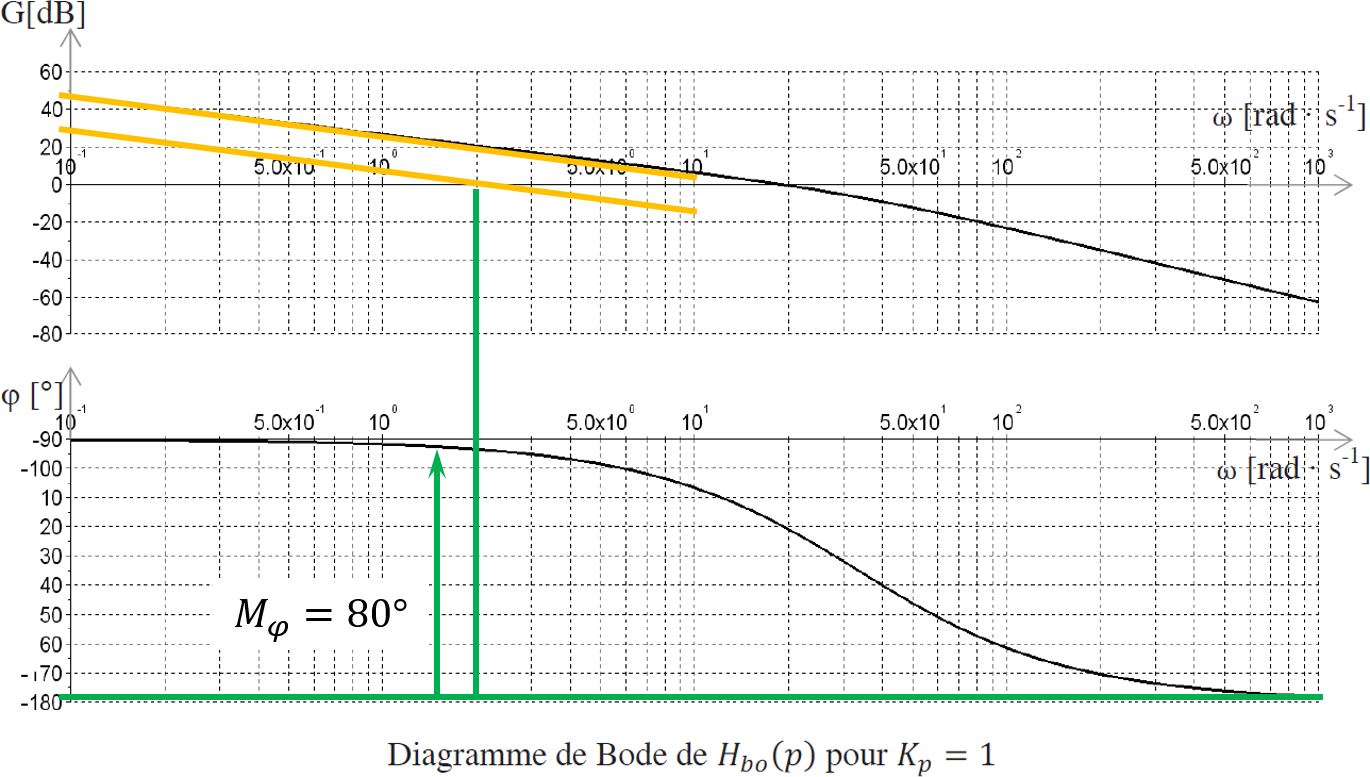
\includegraphics[width=\linewidth]{cor_06}
\end{marginfigure}

La marge de phase est supérieure à 60\degres.
%\end{corrige}
\else
\fi

Afin d'améliorer le comportement, on implante un correcteur Proportionnel Intégral ayant pour fonction de transfert : $H_{\text{cor}}(p)=\frac{K_p\left(1+T_i\cdot p\right)}{T_i\cdot p}$ avec $K_p=1$ et $T_i = \SI{1}{s}$.

\question{Tracer le diagramme de Bode de la fonction de transfert en boucle ouverte avec ce correcteur avec $K_p=1$ et $T_i = \SI{1}{s}$.}% sur la figure \ref{bode_bo_PI}.}
\ifprof
%\begin{corrige}
%\end{corrige}
\else
\fi

\question{On souhaite une marge de phase d'au moins $60^{\circ}$. Proposer un réglage de $K_p$ pour satisfaire au cahier des charges.}% Justifier vos calculs par les tracés nécessaires sur la figure \ref{bode_bo_PI}.}
\ifprof
%\begin{corrige}
%\end{corrige}
\else
\fi

\question{La figure suivante %\ref{reponse_2nd_ordre} 
donne la réponse à un échelon de position de \SI{50}{mm} avec trois types de correcteurs. Vérifier qu'elle est conforme au cahier des charges. Justifier clairement vos réponses en donnant les valeurs numériques pour chaque critère.}
\ifprof

%\begin{corrige} ~\\
\begin{center}
\begin{tabular}{|l|c|c|c|}
\hline
 & P & PI & PID \\  \hline
 Temps de réponse < à 5\,\% < \SI{0,2}{s} &Ok & Ok & Ok \\ \hline
Précision < \SI{1}{mm} & Ok (?) & Ok & Ok \\ \hline
 Dépassement < à 10\,\% < \SI{0,2}{s} & Pas Ok & Pas Ok & Ok \\ \hline
\end{tabular}
\end{center}

\begin{marginfigure}
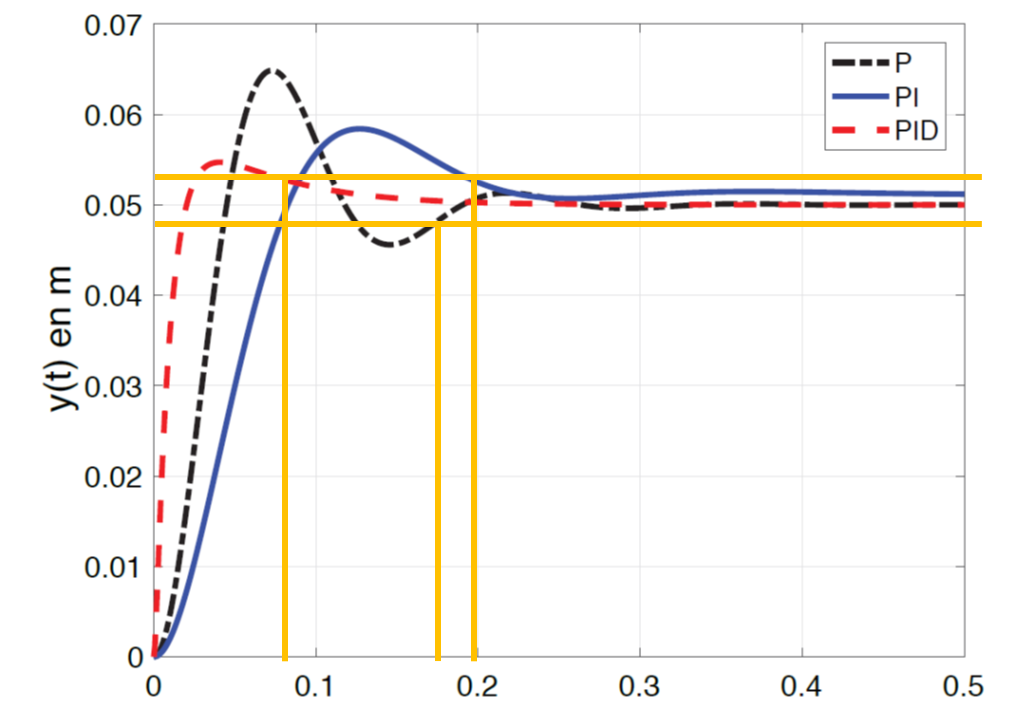
\includegraphics[width=\linewidth]{cor_07}
\end{marginfigure}

%\end{corrige}
\else
\fi

\ifprof
\else
%\begin{figure}[!htb]
\begin{marginfigure}
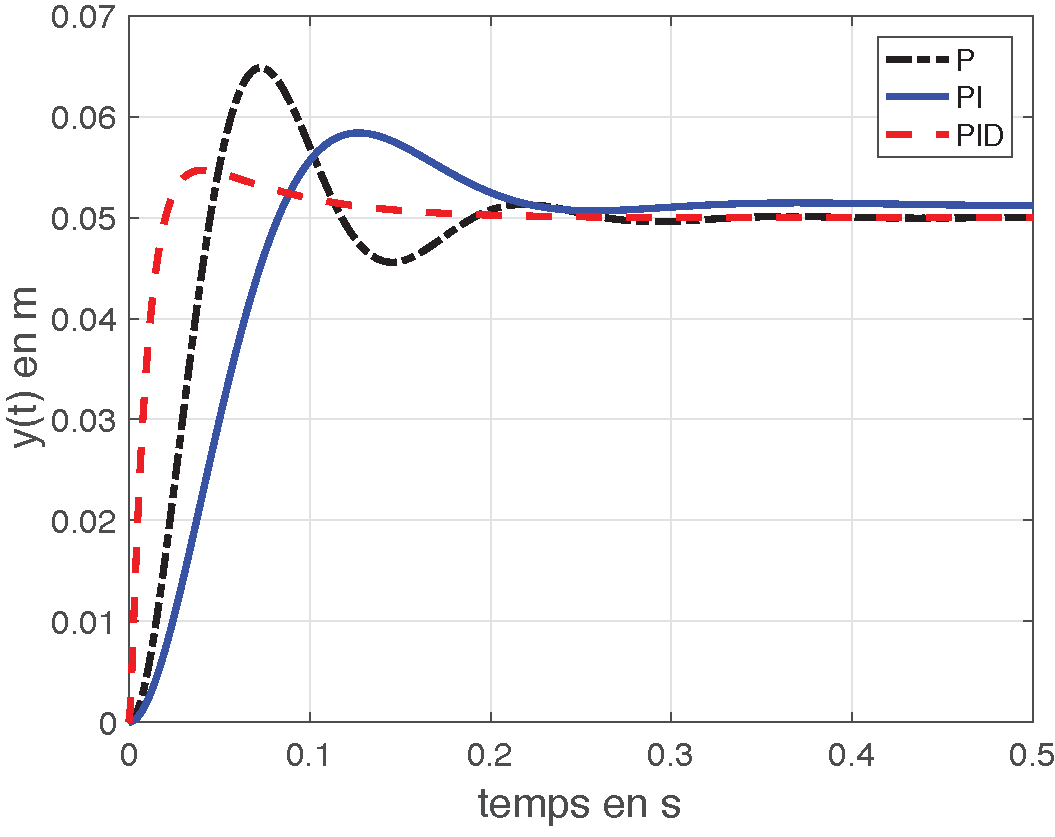
\includegraphics[width=\linewidth]{64_02}
%\caption{Réponse à un échelon de position de $50 mm$ avec trois correcteurs P(question 2) PI (question 5) et PID (déterminé numériquement)\label{reponse_2nd_ordre}}
\end{marginfigure}
%\end{figure}
\fi

\question{Analyser les résultats à l'aide du diagramme de Bode de la FTBO corrigé avec un PID optimisé.}% (figure \ref{bode_pid}.)}
\ifprof
%\begin{corrige}~\\

\begin{marginfigure}
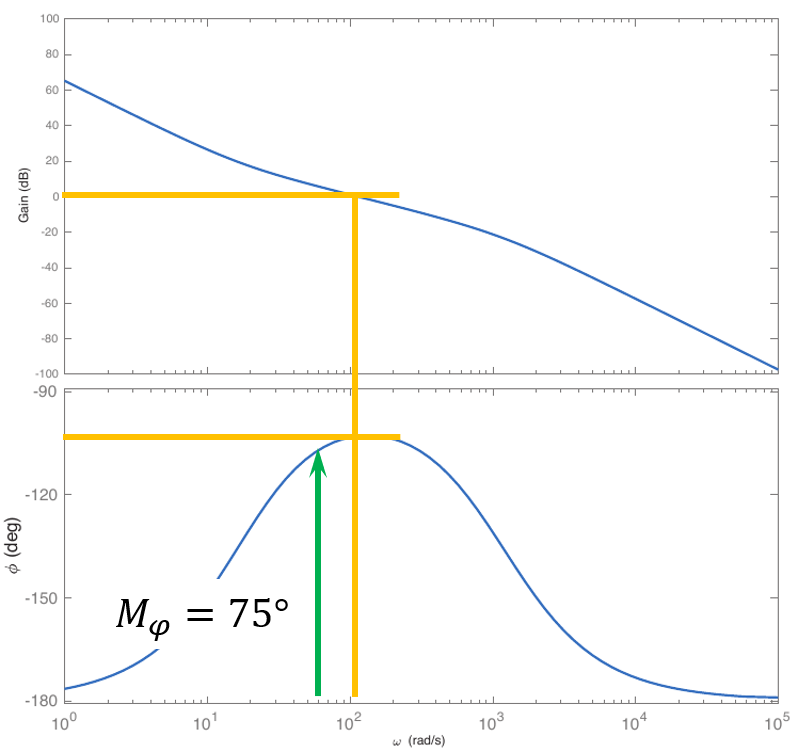
\includegraphics[width=\linewidth]{cor_08}
\end{marginfigure}

La marge de phase est supérieure à 60\degres.

%\end{corrige}
\else
\fi


\ifprof
\else
\begin{marginfigure}
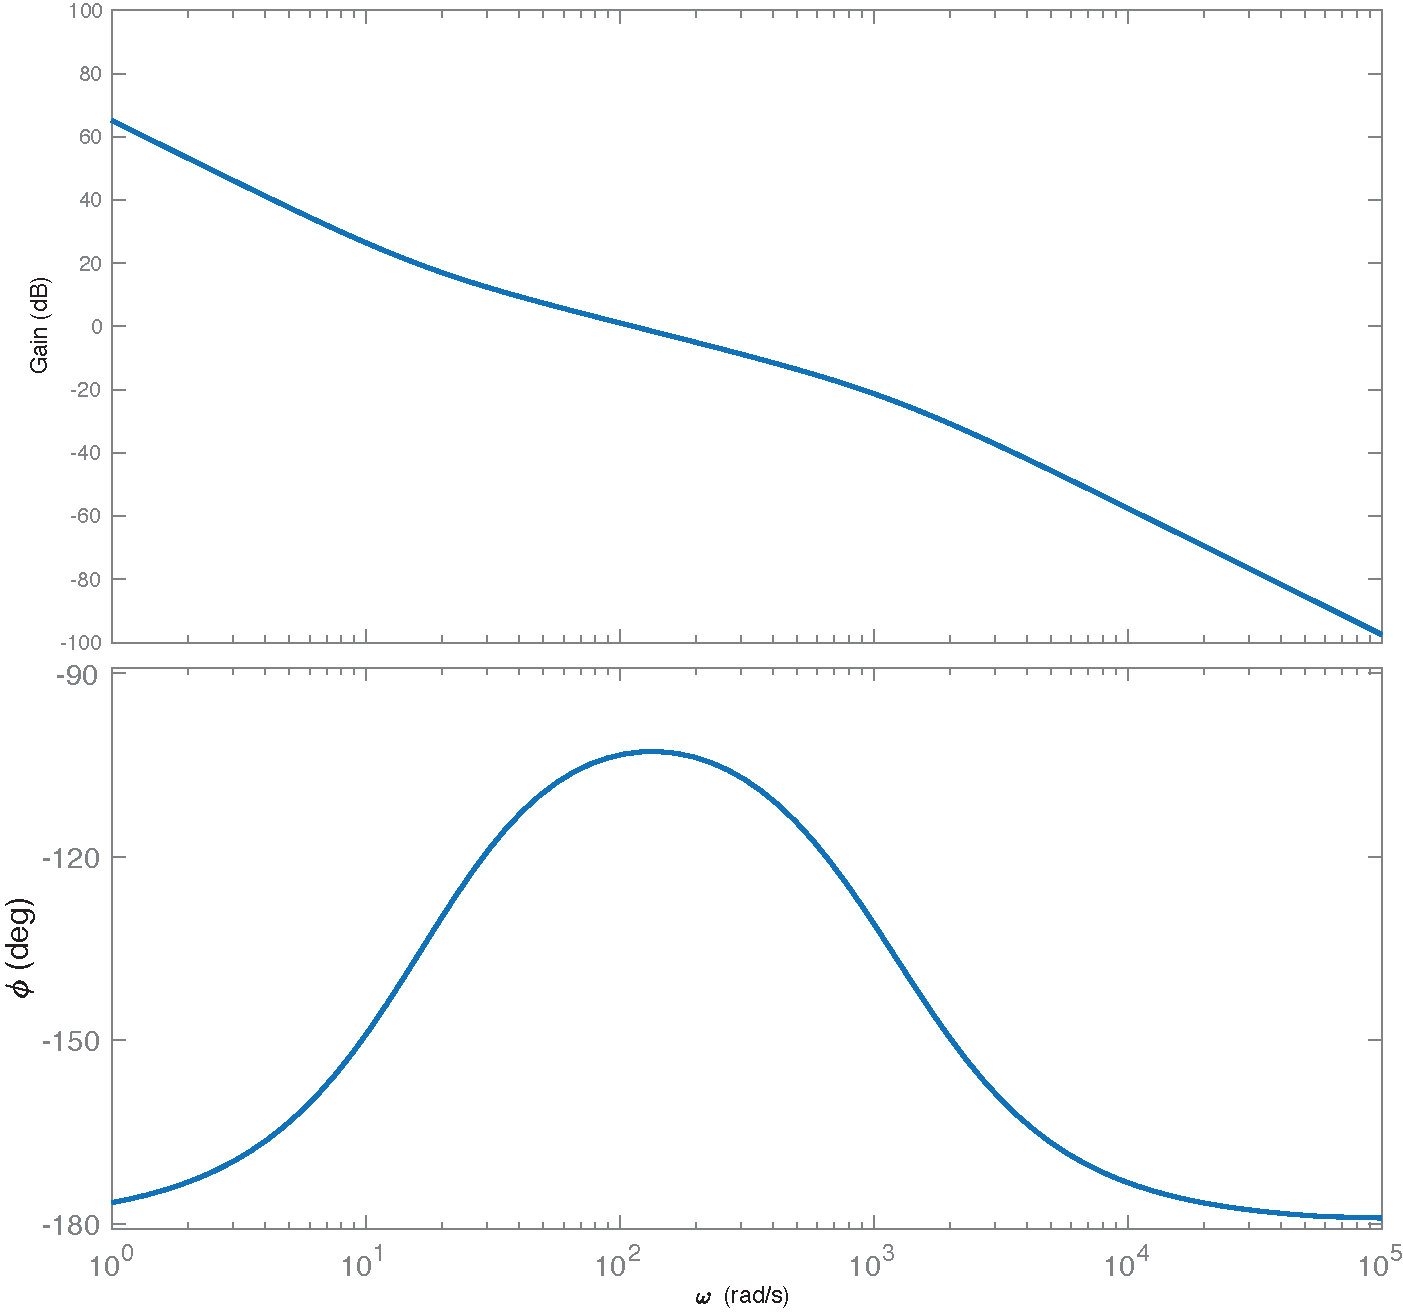
\includegraphics[width=\linewidth]{64_03}
%\caption{Diagramme de Bode de $H_{bo}(p)$ avec un correcteur PID pour $K_p=0,19$, $K_i=2,1$ et $K_d=0,0038$\label{bode_pid}}
\end{marginfigure}
\fi


%%%%%%%%%%%%%%%%%%%%%%%%%%%%%%%
 

\ifprof
\else
%
%\noindent\footnotesize
%\fbox{\parbox{.9\linewidth}{
%Éléments de corrigé : 
%\begin{enumerate}
%  \item $k_{BO}=\sqrt{2}{\tau_m}$.
%    \item $k_c=\dfrac{\sqrt{2}N}{\tau_m k_m k_r} = 471,1$.
%    \item $\varepsilon_s=0$.
%\end{enumerate}}}
%\normalsize


\marginnote{Corrigé voir \ref{PERF:02:C2:03:stab:61}.}

\fi 
 
\graphicspath{{\repStyle/png/}{../PERF/PERF-02-Marges/62_Palettisation/images/}} 
\normaltrue \difficilefalse \tdifficilefalse
\correctiontrue
%\UPSTIidClasse{11} % 11 sup, 12 spé
%\newcommand{\UPSTIidClasse}{11}

\exer{Palettisation -- Stabilité $\star$ \label{PERF:02:C2:03:stab:62}}
%% CCP MP 2010
\setcounter{question}{0}\marginnote{\xpComp{PERF}{02}}%\index{Compétence C2-03}\index{Compétence PERF-02}
\index{Compétence C2-03}
\index{Schéma-blocs}
\index{Stabilité}

\ifcorrection
\else
\marginnote{\textbf{Pas de corrigé pour cet exercice.}}
\fi


\ifprof 
\else
Une boucle de position est représentée ci-dessous. On admet que :  
\begin{itemize}
\item $H(p)=\dfrac{\Omega_m(p)}{U_v(p)}=\dfrac{30}{1+\num{5e-3}p}$;
\item $K_r = \SI{4}{V.rad^{-1}}$ : gain du capteur de position;
\item $K_a$ : gain de l’adaptateur du signal de consigne $\alpha_e(t)$; 
\item $N=200$ : rapport de transmission du réducteur (la réduction est donc de $1/N$).
\item le signal de consigne $\alpha_e(t)$ est exprimé en degré ; 
\item le correcteur $C(p)$ est à action proportionnelle de gain réglable $K_c$. 
\end{itemize}


\begin{center}
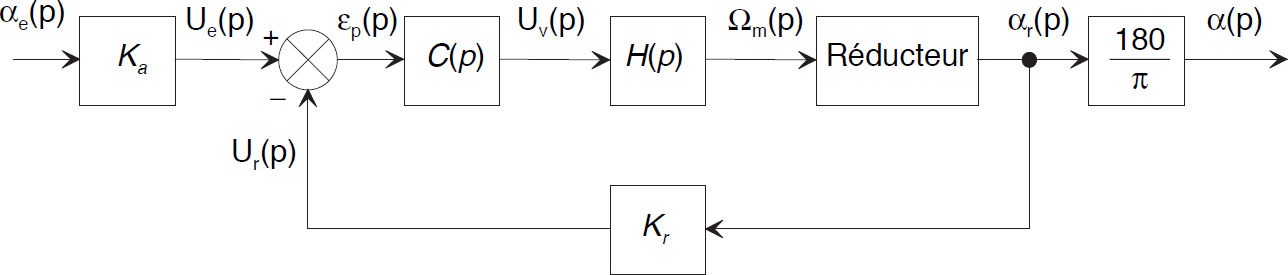
\includegraphics[width=\linewidth]{62_01}
\end{center}
 \fi
 
 
 On montre que la fonction de transfert du réducteur est $R(p)=\dfrac{\alpha_r(p)}{\Omega_m(p)}=\dfrac{1}{Np}$, que  $k_a=\dfrac{\pi}{180}k_r$ et que la FTBO est donnée par $T(p)=\dfrac{k_{BO}}{p\left(1+\tau_m p\right)}$ ($k_{BO}=\dfrac{k_c k_m k_r}{N}$).
 
 
 On souhaite une marge de phase de 45\degres.
 
\question{Déterminer la valeur de $K_{BO}$ permettant de satisfaire cette condition.}
\ifprof
On souhaite une marge de phase de 45\degres. On cherche donc $\omega_{\varphi}$ tel que 
$\varphi\left(\omega_{\varphi}\right)=-180+45 = -135\degres$.

$\varphi(\omega)=-90-\arg\left(1+\tau_m j \omega \right) =-90-\arctan\left(\tau_m  \omega \right)  $.

On a donc $\varphi\left(\omega_{\varphi}\right)=-135$
$\Leftrightarrow -90-\arctan\left(\tau_m  \omega_{\varphi}\right)  = -135 $
$\Leftrightarrow -\arctan\left(\tau_m  \omega_{\varphi} \right)  = -45 $
$\Leftrightarrow \arctan\left(\tau_m  \omega_{\varphi} \right)  = 45 $
$\Rightarrow \tau_m  \omega_{\varphi} = 1 $
$\Rightarrow \omega_{\varphi}  = \dfrac{1}{\tau_m}= \dfrac{1}{5\times 10^{-3}}$
$\Rightarrow \omega_{\varphi}  = \SI{200}{rad.s^{-1}}$.


Par suite, il faut que le gain soit nul en $\omega_{\varphi}$.

On a donc $\indice{G}{dB}(\omega)=20\log k_{BO}-20\log\omega-20\log\sqrt{1+\omega^2\tau_m^2}$.
En $\omega_{\varphi} =  \dfrac{1}{\tau_m}$ :
$\indice{G}{dB}(\omega_{\varphi})=0$ 
$\Leftrightarrow 20\log k_{BO}-20\log \dfrac{1}{\tau_m}-20\log\sqrt{1+\dfrac{1}{\tau_m^2}\tau_m^2}=0$
$\Leftrightarrow \log k_{BO}+\log \tau_m-\log\sqrt{2}=0$
$\Leftrightarrow \log \dfrac{k_{BO} \tau_m}{\sqrt{2}}=0$
$\Leftrightarrow \dfrac{k_{BO} \tau_m}{\sqrt{2}}=1$
$\Leftrightarrow k_{BO}=\dfrac{\sqrt{2}}{\tau_m}$.

(\textbf{A vérifier})
$k_{BO}=282,8$.

\else 
\fi

\question{En déduire la valeur du gain $K_c$ du correcteur. }
\ifprof
$k_{BO}=\dfrac{k_c k_m k_r}{N}$; donc 
$k_c=\dfrac{Nk_{BO}}{ k_m k_r} = \dfrac{200 \times 282,8 }{4\times 30}=471$.
\else 
\fi

\question{Déterminer l’écart de position.}
\ifprof
Il y a une intégration dans la correcteur. La FTBO est de classe 1 est le système est précis en position. 
\else 
\fi

 

\ifprof
\else

\marginnote{\begin{solution}
\begin{enumerate}
  \item $k_{BO}=\dfrac{\sqrt{2}}{\tau_m}$.
  \item $k_c=\dfrac{\sqrt{2}N}{\tau_m k_m k_r} = 471,1$.
  \item $\varepsilon_s=0$.
\end{enumerate}
\end{solution}}


\marginnote{Corrigé voir \ref{PERF:02:C2:03:stab:62}.}

\fi 
 
\graphicspath{{\repStyle/png/}{../PERF/PERF-02-Marges/63_BancHydraulique/images/}} 
\normalfalse \difficiletrue \tdifficilefalse
\correctiontrue
%\UPSTIidClasse{11} % 11 sup, 12 spé
%\newcommand{\UPSTIidClasse}{11}

\exer{Banc hydraulique $\star$ \label{PERF:02:C2:03:stab:63}}
%% CCP MP 2010
\setcounter{question}{0}\marginnote{\xpComp{PERF}{02}}%\index{Compétence C2-03}\index{Compétence PERF-02}
\index{Compétence C2-03}
\index{Schéma-blocs}
\index{Précision}

\ifcorrection
\else
\marginnote{\textbf{Pas de corrigé pour cet exercice.}}
\fi

\ifprof
\else

Pour limiter l’erreur statique due aux fuites, on envisage d’asservir la pression d’eau dans le tube. 
%L’objectif est ici de proposer un réglage du correcteur pour répondre aux critères du cahier des charges.
La pression d’eau à l’intérieur du tube est mesurée par un capteur de pression. 

\begin{marginfigure}
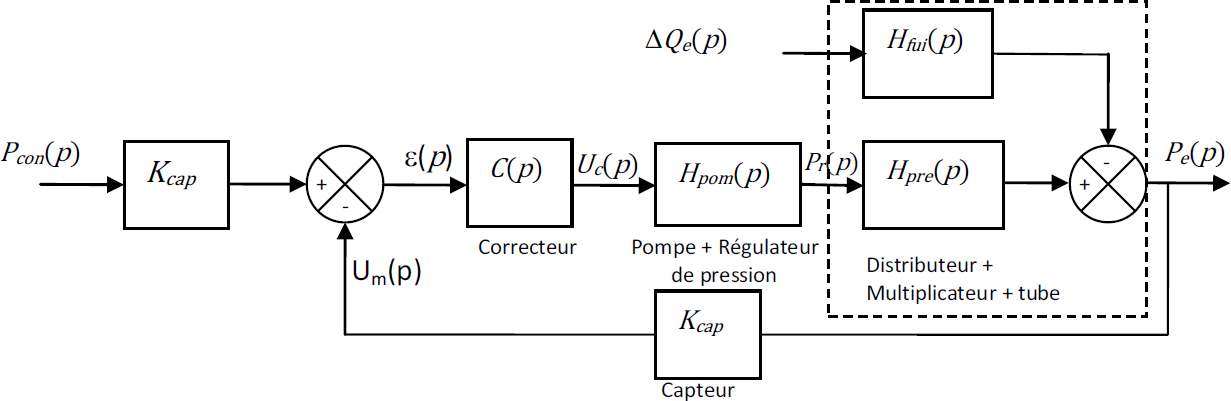
\includegraphics[width=\linewidth]{63_01}
\end{marginfigure}

 
 \begin{tabular}{lp{5cm}}
$P_{\text{con}}(p)$ : & 	pression de consigne d’eau dans le tube (Pa) \\
$P_e(p)$ : & 	pression d’eau dans le tube (Pa) \\
$U_c(p)$ : & 	tension de commande du régulateur de pression (V)\\
$P_r(p)$ : &	pression d’huile régulée (Pa)\\
$\Delta Q_e(p)$ :& 	débit de fuite (\si{m^3s^{-1}})\\
$U_m(p)$ 	:&	tension de mesure du capteur (V)\\
\end{tabular}
 
\textbf{ Hypothèses}
\begin{itemize}
\item L’ensemble de mise sous pression {tube + distributeur + multiplicateur de pression} est défini par les transmittances suivantes : $H_{\text{pre}} (p)=\dfrac{K_m}{1+T_1 p}$	et	$H_{\text{fui}} (p)=\dfrac{K_f}{1+T_1 p}$ avec 	$K_m = 3,24$ ; 	$K_f = \SI{2,55e10}{Pa.m^{-3}.s}$ ; 	$T_1  = \SI{10}{s}$.
\item L’ensemble {pompe+régulateur de pression} est modélisé par la fonction de transfert :
$H_{\text{pom}} (p)=\dfrac{K_{\text{pom}}}{1+T_2 p}$  avec 	$K_{\text{pom}} = \SI{1,234e7}{Pa/V}$; 	$T_2 = \SI{5}{s}$.
\item Le capteur est modélisé par un gain pur :	$K_{\text{cap}} = \SI{2,5e-8}{V/Pa}$.
\end{itemize}
La pression de consigne est de $P_{\text{con}} = \SI{800}{bars}$ et les débits de fuite sont estimés à $\Delta Q_e = \SI{5e-4}{m3/s}$.

 
Le cahier des charges concernant le réglage de la pression de test est le suivant.
\begin{center}
\begin{tabular}{ll}
\hline 
Stabilité :  & marge de phase de 60\degres  \\
  	  &  marge de gain de \SI{12}{dB} \\ \hline
Rapidité :  &  temps d’établissement $t_e < \SI{40}{s}$ (voir remarque ci-dessous) \\ \hline
Précision : & 	erreur statique < 5\% soit pour une consigne de 800 bars : \\
&erreur statique due à la consigne : $\varepsilon_{\text{con}}< 5\%$  \\
& erreur statique due à la perturbation $\varepsilon_{\text{pert}} < \SI{40}{bars}$ \\ \hline
Amortissement :&	pas de dépassement \\ \hline
\end{tabular}
\end{center}

Dans le cas d’un système bouclé convenablement amorti, on pourra utiliser, sans aucune justification, la relation :
$t_e \cdot \omega_{\SI{0}{dB}}=3$ où $\omega_{\SI{0}{dB}}$ désigne la pulsation de coupure à \SI{0}{dB} en boucle ouverte et $t_e$ le temps d’établissement en boucle fermée vis-à-vis d’un échelon de consigne :
\begin{itemize}
\item $t_e = t_m$, temps du 1er maximum si le dépassement est supérieur à \SI{5}{\%},
\item $t_e = t_R$, temps de réponse à \SI{5}{\%} si le dépassement est nul ou inférieur à \SI{5}{\%}.
\end{itemize}

On se propose de corriger le système avec le correcteur défini sur le schéma bloc ci-dessous.

\begin{marginfigure}
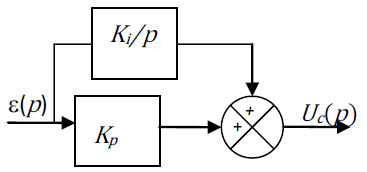
\includegraphics[width=5cm]{63_02}
\end{marginfigure}
\fi

\question{Déterminer la fonction de transfert $C(p)$ de ce correcteur.}
\ifprof
On a $C(p)=\dfrac{K_i}{p}+K_p = \dfrac{K_i+p K_p}{p} = K_i \dfrac{1+p \dfrac{K_p}{K_i}}{p}$.
\else 
\fi


\question{Tracer l’allure de son diagramme de Bode en fonction des coefficients $K_i$ et $K_p$.}
\ifprof

\begin{marginfigure}
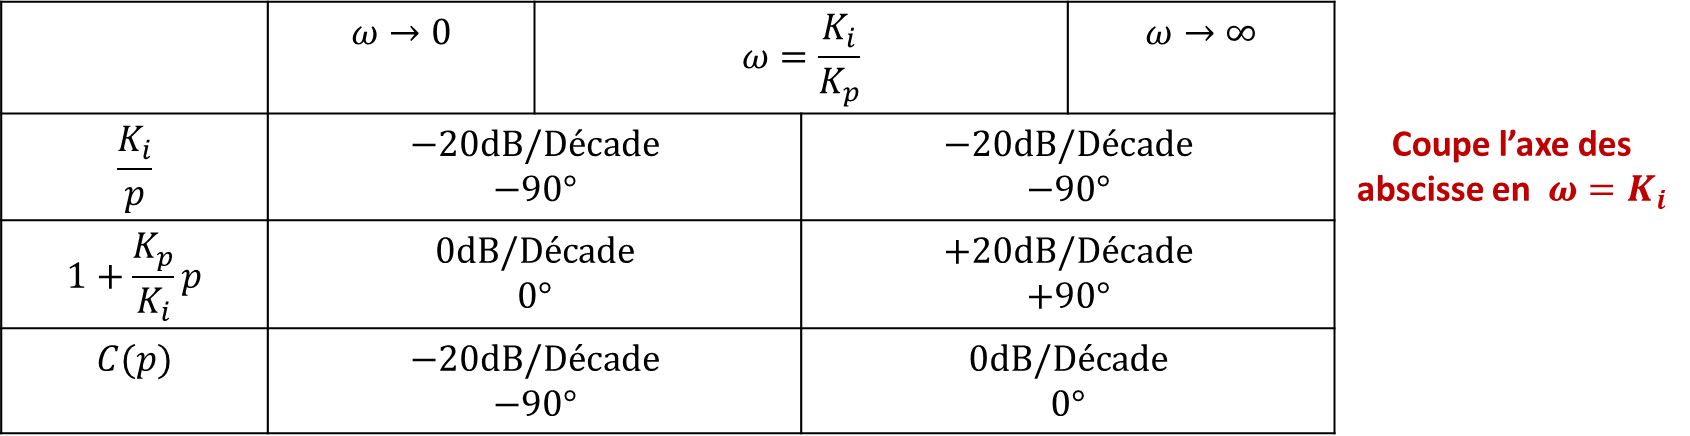
\includegraphics[width=\linewidth]{63_02_cor}
\end{marginfigure}

\begin{marginfigure}
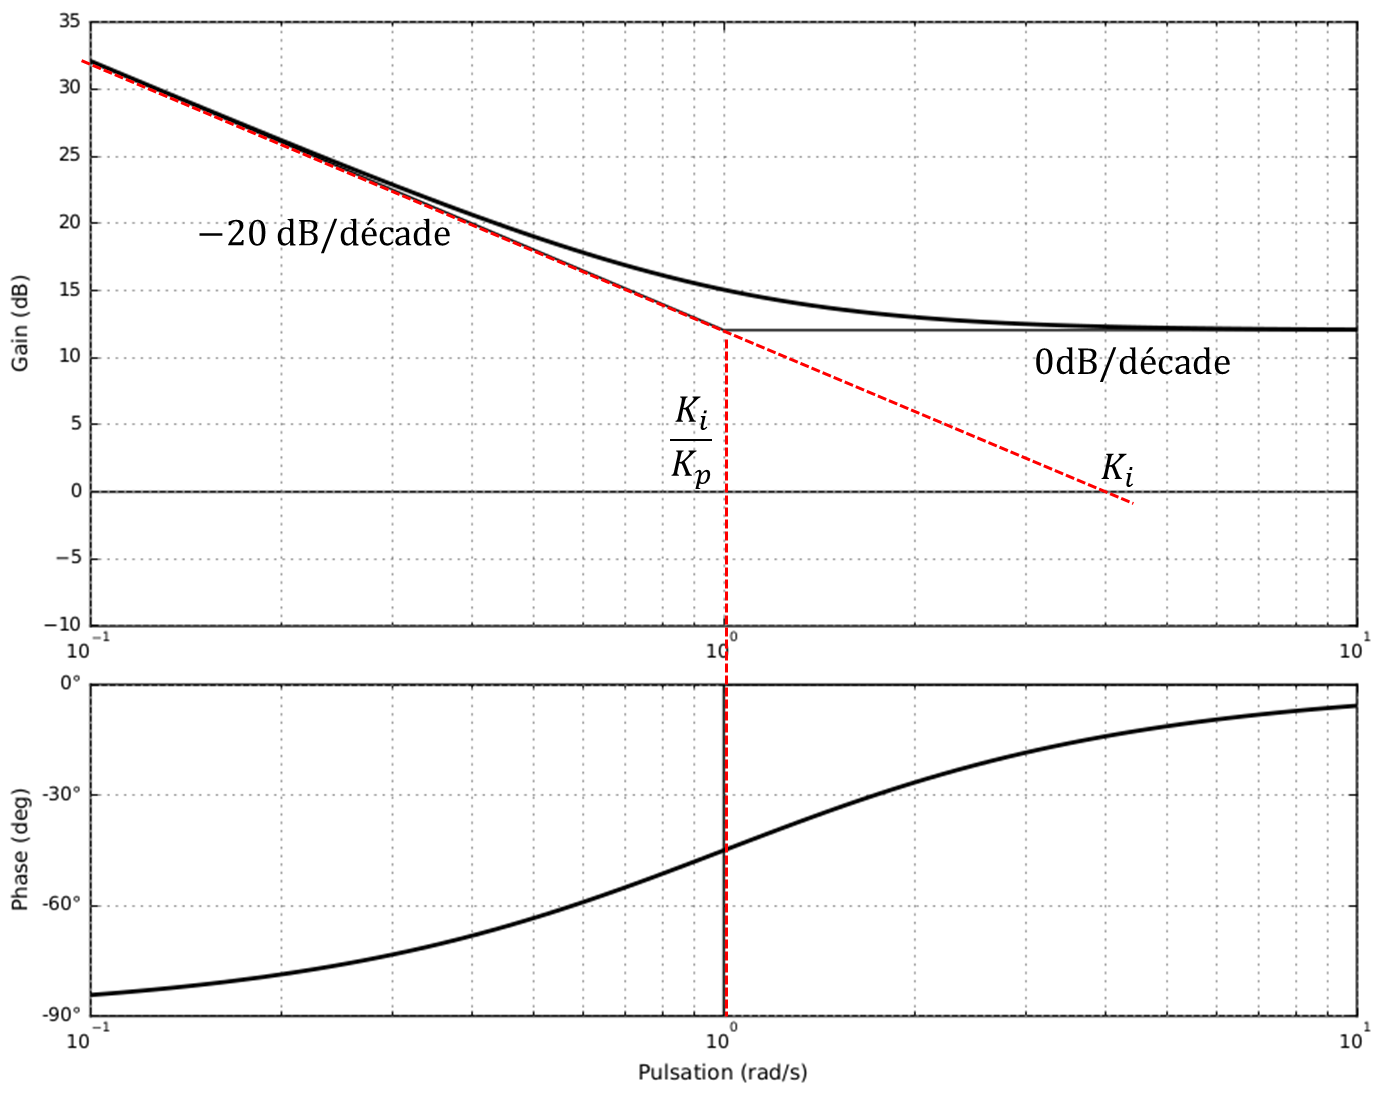
\includegraphics[width=\linewidth]{63_03_cor}
\end{marginfigure}


\else 
\fi


\question{Quelle est l’influence d’un tel correcteur sur la précision et la stabilité ? Justifier.}
\ifprof
Ce correcteur augmente la classe de la FTBO donc augmente la précision. 
Cependant, il réduit la phase. Il faut donc veiller à ce que la pulsation de cassure soit réglée de telle sorte que le système ne soit pas déstabilisé. 
\else 
\fi


\question{Quelle valeur faut-il donner à $\omega_{\SI{0}{dB}}$ pour répondre au critère de rapidité du cahier des charges ?}
\ifprof
D'après la remarque, on a $t_e \omega_{\SI{0}{dB}}=3$ soit $\omega_{\SI{0}{dB}} =3/t_e = \SI{0,075}{rad.s^{-1}}$.
\else 
\fi


\question{Déterminer analytiquement le rapport $T=\dfrac{K_p}{K_i}$ pour obtenir la marge de phase spécifiée dans le cahier des charges.}
\ifprof
Calculons la fonction de transfert en boucle ouverte non corrigée : 
$\indice{F}{BO}=\dfrac{\indice{K}{pom}}{1+T_2 p}\dfrac{\indice{K}{m}}{1+T_1 p} \indice{K}{cap}$.

Le correcteur doit être réglé pour que $\omega_{\SI{0}{dB}} =\SI{0,075}{rad.s^{-1}}$. 

Calculons la marge de phase. 
$\arg\left(\indice{F}{BO}\right)=-\arg\left(1+T_1p\right)-\arg\left(1+T_2p\right) = -\arctan T_1 \omega -\arctan T_2 \omega $
+
On a donc $\arg\left(\indice{F}{BO}(0,075)\right) = -\arctan (10 \times  0,075) -\arctan (5 \times  0,075)=-57\degres$ soit une marge de phase de $-123\degres$.

Pour atteindre une marge de phase de 60\degres, on peut donc baisser la phase de 63\degres.

Calculons $\arg\left(C(j\omega)\right)=-90+\arctan \left(\dfrac{K_p}{K_i}\omega\right)$.

On cherche donc $\dfrac{K_i}{K_p}$ tel que $\arg\left(C(0,075)\right)=-63$
Soit 
$-90+\arctan \left(\dfrac{K_p}{K_i}0,075\right) =-63$
$\Leftrightarrow \arctan \left(\dfrac{K_p}{K_i}0,075\right) =27$
$\Rightarrow  \dfrac{K_p}{K_i}0,075 =0,51$
$\Leftrightarrow  \dfrac{K_p}{K_i}=6,79$.


\else 
\fi


\question{En déduire les valeurs de $K_i$ et $K_p$ qui permettent de régler rapidité et marge de phase.}
\ifprof
Il faut chercher $K_i$ et $K_p$ pour respecter $\omega_{\SI{0}{dB}}$. Recherchons le gain de la boucle ouverte non corrigée pour $\omega_{\SI{0}{dB}}$.

$\indice{G}{dB}\left(\indice{F}{BO}\right)=20\log\left(\indice{K}{pom}\indice{K}{m}\indice{K}{cap}\right)
-20\log\left(\sqrt{1^2+T_1^2\omega^2}\right)-20\log\left(\sqrt{1^2+T_2^2\omega^2}\right)$

On a alors $\indice{G}{dB}\left(\indice{F}{BO}\right)(0,075) = -0,004-1,94-0,57=\SI{2,52}{dB}$.

Il faut donc baisser le gain de \SI{2,52}{dB}
$\indice{G}{dB}\left(C(p)\right)$  
$= 20\log K_i -20\log \omega +20\log\left(\sqrt{1+\left(\dfrac{K_p}{K_i}\right)^2\omega^2}\right) $.

On a alors $\indice{G}{dB}\left(C(0,075)\right) = 20\log K_i +22,5+1 = -2,52$ soit $K_i = 10^{-\dfrac{2,52+1+22,5}{20}  } =0,05$.

Par suite, $K_p = 6,79 \times 0,05 = 0,34$.

(\textbf{A vérifier}).

\else 

On donne les diagrammes de Bode en gain et en phase de la fonction de transfert en boucle ouverte corrigée avec le correcteur Proportionnel Intégral déterminé précédemment. On donne sa réponse temporelle avec et sans débit de fuite pour une pression de consigne d’eau de 800 bars.

\fi



\question{La réponse du système est-elle satisfaisante au regard du cahier des charges ? Justifier.}
\ifprof
\begin{marginfigure}
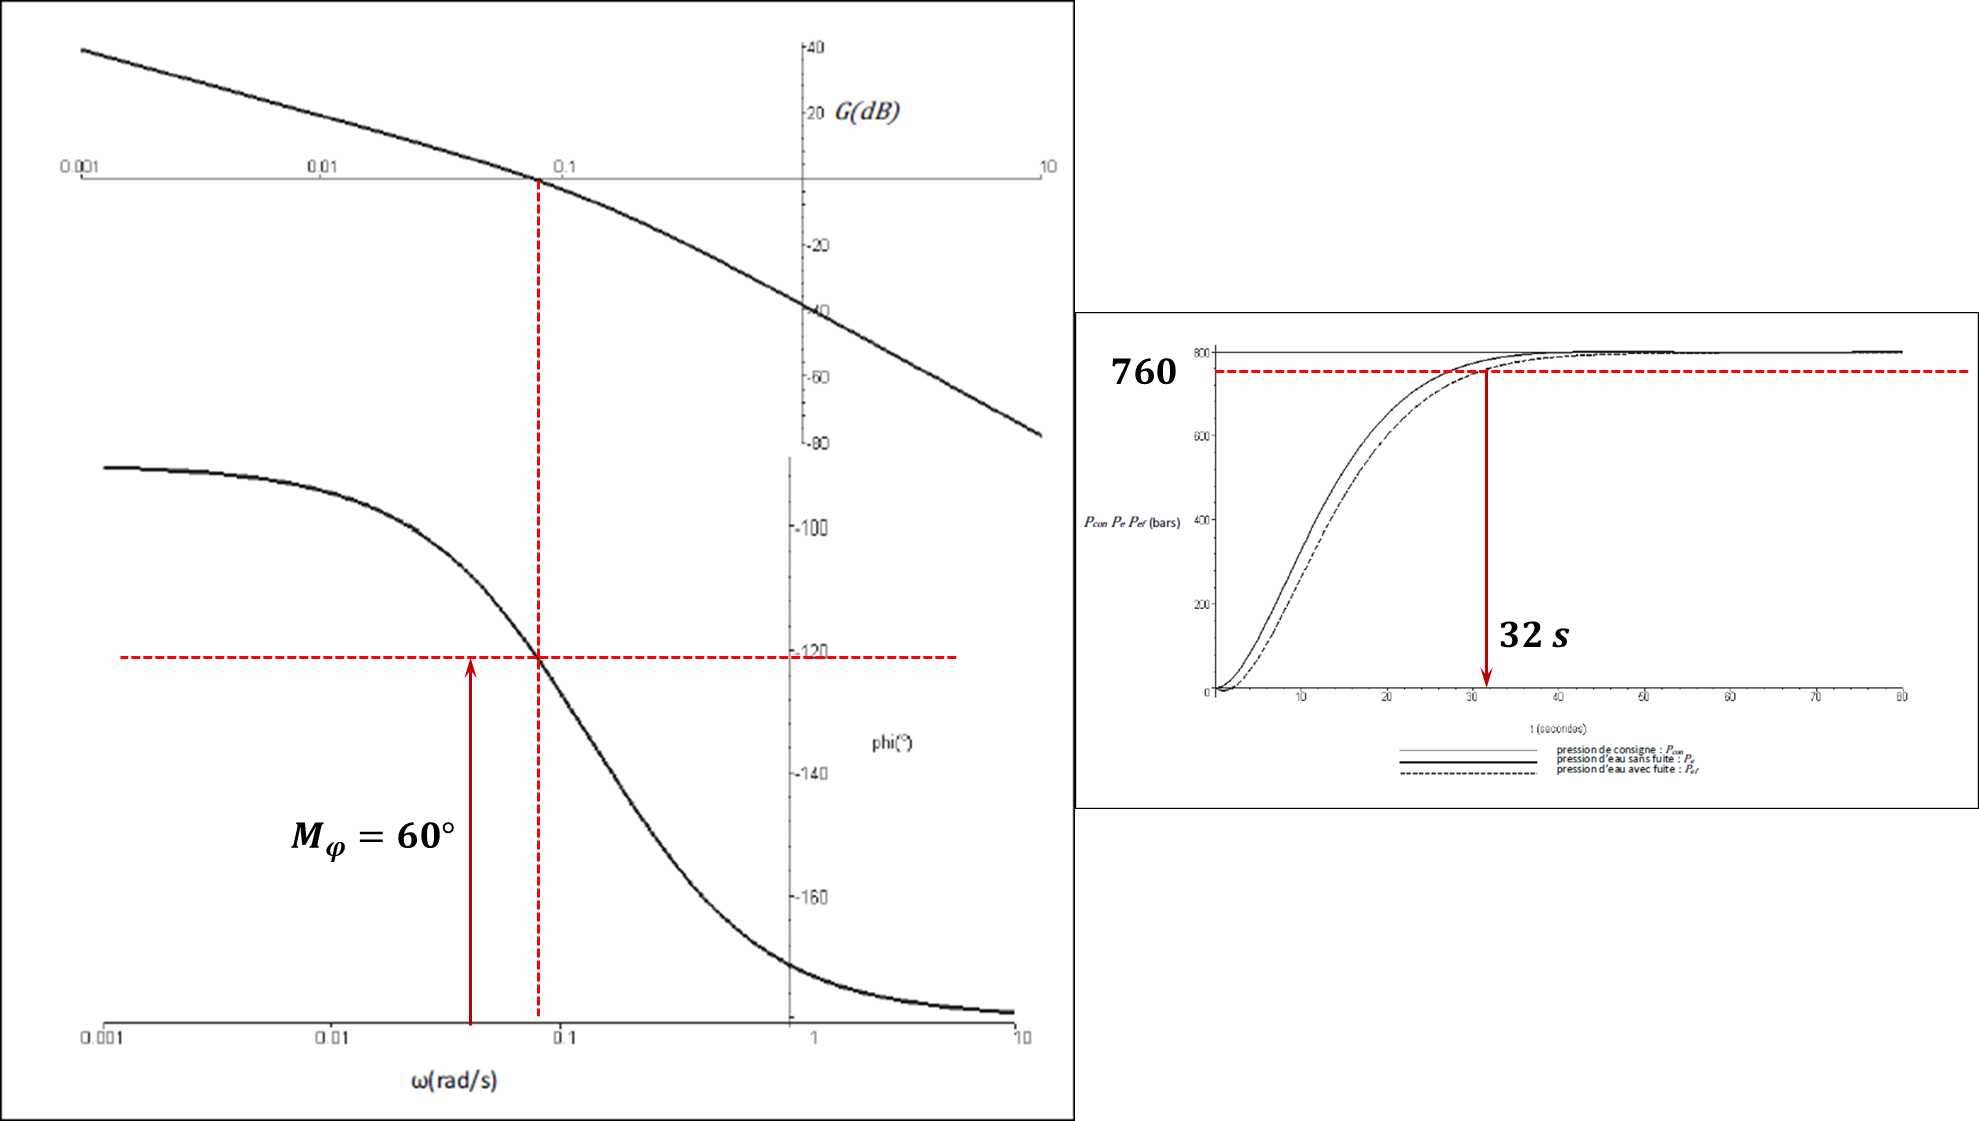
\includegraphics[width=\linewidth]{63_04_cor}
\end{marginfigure}
\begin{itemize}
\item Stabilité : 
\begin{itemize}
\item Marge de phase mesurée :  60\degres \textbf{cdc ok}.
\item Marge de gain mesurée :   infini \textbf{cdc ok}.
\end{itemize}
\item Rapidité : $ t_e = \SI{32}{s} < \SI{40}{s}$ \textbf{cdc ok}.
\item Précision :  écart statique nul \textbf{cdc ok}.
\item Amortissement :  nul \textbf{cdc ok}.
\end{itemize}
\else 
\fi

\ifprof
\else

\begin{marginfigure}
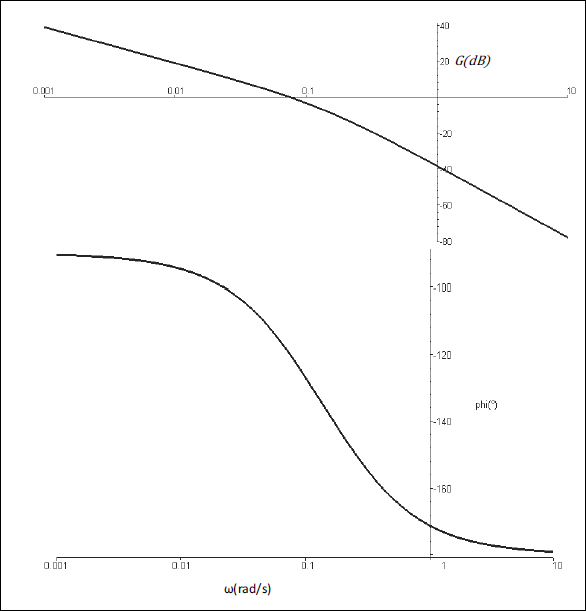
\includegraphics[width=\linewidth]{63_03}
\end{marginfigure}


\begin{marginfigure}
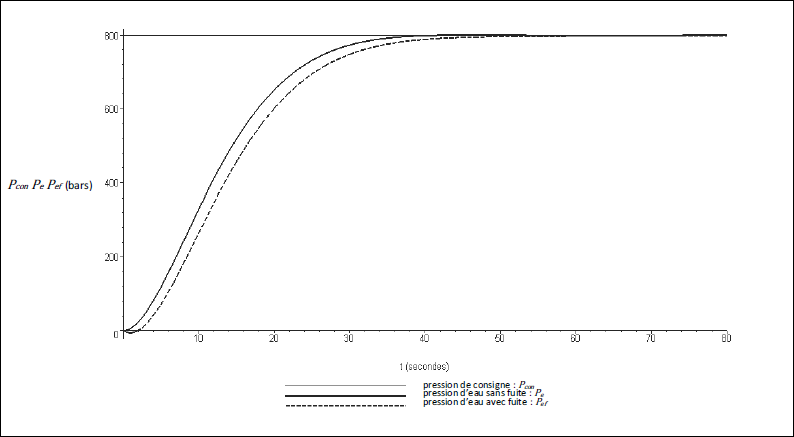
\includegraphics[width=\linewidth]{63_04}
\end{marginfigure}
\fi

\ifprof
\else

\marginnote{\begin{solution} 
\begin{enumerate}
  \item $C(p)= K_i \dfrac{1+p \dfrac{K_p}{K_i}}{p}$.
  \item .
  \item .
  \item $T = 6,79$.
  \item $K_i = 0,05$ et $K_p=0,34$ (à vérifier).
\end{enumerate}
\end{solution}}

\marginnote{Corrigé voir \ref{PERF:02:C2:03:stab:63}.}

\fi 
 
\graphicspath{{\repStyle/png/}{../PERF/PERF-02-Marges/64_EPAS/images/}} 
\normaltrue \difficilefalse \tdifficilefalse
\correctionfalse
%\UPSTIidClasse{11} % 11 sup, 12 spé
%\newcommand{\UPSTIidClasse}{11}

\exer{Exercice d'application $\star$ \label{PERF:02:C2:03:stab:64}}
%% CCP MP 2007
\setcounter{question}{0}\marginnote{\xpComp{PERF}{02}}%\index{Compétence C2-03}\index{Compétence PERF-02}
\index{Compétence C2-03}
\index{Schéma-blocs}
\index{Stabilite}

\ifcorrection
\else
\marginnote{\textbf{Pas de corrigé pour cet exercice.}}
\fi


\ifprof
\else
L'asservissement est donné par le schéma-blocs suivant. $H_{\text{BO}}(p) = \dfrac{4}{p\left( p+3,6\right)}$.  Le retard du système est de \SI{0,2}{s}.
De plus, $C(p)=K_c\dfrac{1+T_c p}{T_c p}$

\begin{marginfigure}
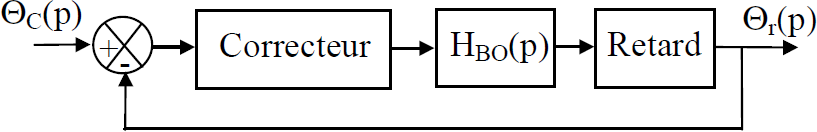
\includegraphics[width=\linewidth]{64_01}
\end{marginfigure}

\fi
 
\question{Tracer le diagramme de Bode asymptotique de $H_{\text{BO}}(p)$ pour des pulsations comprises entre \SI{0,5}{rad.s^{-1}} et \SI{50}{rad.s^{-1}}.}
\ifprof
\else 
\fi

\question{Tracer le diagramme de Bode du retard pour des pulsations comprises entre \SI{0,5}{rad.s^{-1}} et \SI{50}{rad.s^{-1}}.}
\ifprof
\else 
\fi


\ifprof
\else
On donne le diagramme de la FTBO retardée. 

\begin{marginfigure}
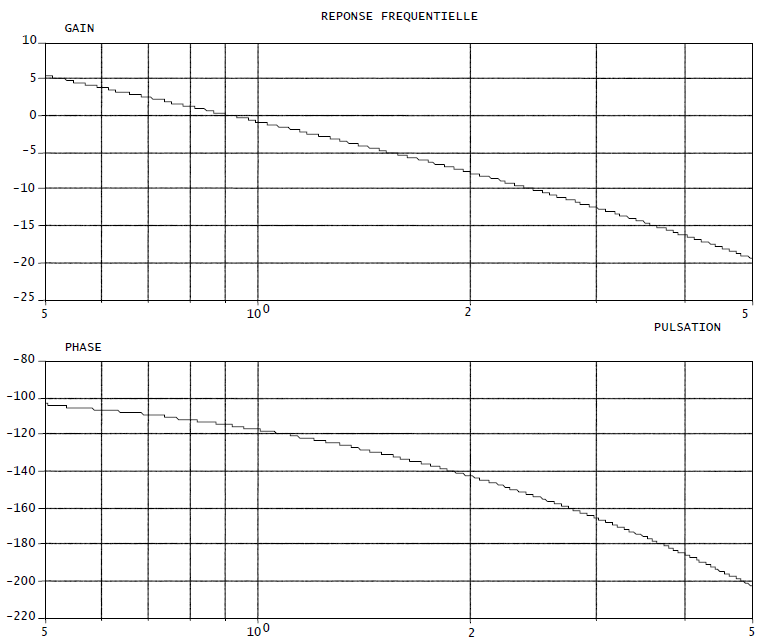
\includegraphics[width=\linewidth]{64_02}
\end{marginfigure}
\fi

\question{Déterminer le gain $K_c$ qui donne une marge de phase de 50\degres.}
\ifprof
\else 
\fi

\question{La constante $T_c$ qui laisse subsister une marge de phase d’environ 45\degres.}
\ifprof
\else 
\fi


\question{Quelle est l’erreur de traînage du système corrigé pour l’entrée en rampe considérée (en négligeant le retard).}
\ifprof
\else 
\fi


\ifprof
\else



\marginnote{Corrigé voir \ref{PERF:02:C2:03:stab:64}.}

\fi 
 
\section{Évaluer la rapidité de la réponse temporelle} 
\section{Évaluer la rapidité à partir de la réponse fréquentielle de la BO} 
\section{Évaluer la précision à partir du TVF} 
\graphicspath{{\repStyle/png/}{../PERF/PERF-05-Precistion-TVF/501_Divers/images/}} 
\normaltrue \difficilefalse \tdifficilefalse
\correctiontrue

%\UPSTIidClasse{11} % 11 sup, 12 spé
%\newcommand{\UPSTIidClasse}{11}

\exer{Valeur finale$\star$ \label{PERF:05:C2:03:501}}
\setcounter{question}{0}\marginnote{\xpComp{PERF}{05}}%\UPSTIcompetence[2]{C2-03}
\index{Compétence C2-03}
\index{Schéma-blocs}
\index{Valeur finale}

\ifcorrection
\else
\marginnote{\textbf{Pas de corrigé pour cet exercice.}}
\fi


\ifprof 
\else
Soit le schéma-blocs suivant.
\begin{marginfigure}
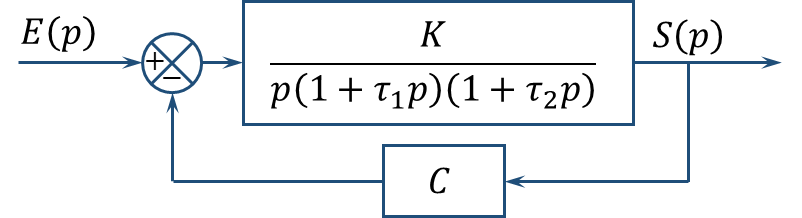
\includegraphics[width=\linewidth]{501_01}
\end{marginfigure}
 \fi
 
\question{Déterminer la valeur finale de $s(t)$ lorsque l'entrée est un échelon d'amplitude $E_0$.}
\ifprof

On a 
$H(p)=\dfrac{\dfrac{K}{p\left(1+\tau_1 p \right)\left(1+\tau_2 p \right)}}{1+\dfrac{CK}{p\left(1+\tau_1 p \right)\left(1+\tau_2 p \right)}}$
$=\dfrac{K}{p\left(1+\tau_1 p \right)\left(1+\tau_2 p \right)+CK}$. 
En conséquence, $S(p)=E(p)\dfrac{K}{p\left(1+\tau_1 p \right)\left(1+\tau_2 p \right)+CK}$.

$s_{\infty}=\lim\limits_{t\to +\infty} s(t)$ $=\lim\limits_{p\to 0} pS(p)$
$=\lim\limits_{p\to 0} pE(p)H(p)$.
Dans le cas où $E(p)$ est un échelon, on a $E(p)=\dfrac{E_0}{p}$ et donc 
$s_{\infty}=\lim\limits_{p\to 0} p\dfrac{E_0}{p}\dfrac{K}{p\left(1+\tau_1 p \right)\left(1+\tau_2 p \right)+CK}=\dfrac{E_0}{C}$.
\else 
\fi

%\question{En déduire la valeur de l'erreur statique.}
%\ifprof
%L'erreur statique est donnée par $\lim\limits_{t\to +\infty} (e(t)-s(t))=E_0 - \dfrac{E_0}{C}$.
%\else
%\fi

\question{Déterminer la valeur finale de $s(t)$ lorsque l'entrée est une rampe de pente $k$.}
\ifprof

On a maintenant $E(p)=\dfrac{k}{p^2}$. 
On a donc et donc 
$s_{\infty}=\lim\limits_{p\to 0} p\dfrac{k}{p^2}\dfrac{K}{p\left(1+\tau_1 p \right)\left(1+\tau_2 p \right)+CK}$ et 
$s_{\infty}=\infty$.

\else 
\fi


%\question{En déduire la valeur de l'erreur de traînage.}
%\ifprof
%$\varepsilon_v = \lim\limits_{t\to +\infty} (e(t)-s(t))$
%$=\lim\limits_{p\to 0} p\left(\dfrac{k}{p^2}-\dfrac{k}{p^2}\dfrac{K}{p\left(1+\tau_1 p \right)\left(1+\tau_2 p \right)+CK}\right)$
%
%$=\lim\limits_{p\to 0} \dfrac{k}{p}\left(1-\dfrac{K}{p\left(1+\tau_1 p \right)\left(1+\tau_2 p \right)+CK}\right)$
%$=\lim\limits_{p\to 0} \dfrac{k}{p}\dfrac{p\left(1+\tau_1 p \right)\left(1+\tau_2 p \right)+CK-K}{p\left(1+\tau_1 p \right)\left(1+\tau_2 p \right)+CK}=+\infty$
%\else
%\fi
%
%\question{Qu'en est-il si $C=1$ ?.}
%\ifprof
%$\varepsilon_v =\lim\limits_{p\to 0} \dfrac{k}{p}\dfrac{p\left(1+\tau_1 p \right)\left(1+\tau_2 p \right)+CK-K}{p\left(1+\tau_1 p \right)\left(1+\tau_2 p \right)+CK}$
%$=\lim\limits_{p\to 0} \dfrac{k}{p}\dfrac{p\left(1+\tau_1 p \right)\left(1+\tau_2 p \right)}{p\left(1+\tau_1 p \right)\left(1+\tau_2 p \right)+K}$
%$=\lim\limits_{p\to 0} k\dfrac{\left(1+\tau_1 p \right)\left(1+\tau_2 p \right)}{p\left(1+\tau_1 p \right)\left(1+\tau_2 p \right)+K} = \dfrac{k}{K}$.


%
%\else
%\fi
%\question{Réaliser le schéma-blocs.}
%\ifprof
%\begin{figure}[H]
%\centering
%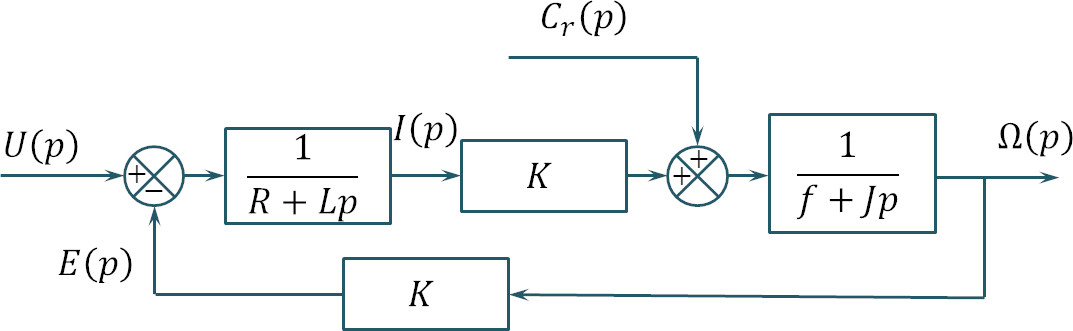
\includegraphics[width=\linewidth]{51_01_c}
%%\caption{Évolution du couple utile en fonction de la vitesse de rotation pour des
%%fréquences de commande de \SI{90}{Hz} à \SI{110}{Hz}. \label{fig_50_04}}
%\end{figure}
%\else
%\fi


 

\ifprof
\else
\marginnote{\begin{solution} 
\begin{enumerate}
    \item $s_{\infty}=\lim\limits_{p\to 0} p\dfrac{E_0}{p}\dfrac{K}{p\left(1+\tau_1 p \right)\left(1+\tau_2 p \right)+CK}=\dfrac{E_0}{C}$.
   % \item $\lim\limits_{t\to +\infty} (e(t)-s(t))=E_0 - \dfrac{E_0}{C}$.
    \item $s_{\infty}=\infty$.
   % \item $\varepsilon_v =\infty$.
%    \item $\varepsilon_v =\dfrac{k}{K}$.
\end{enumerate}
\end{solution}}

\marginnote{Corrigé voir \ref{PERF:05:C2:03:501}.}

\fi 
 
\graphicspath{{\repStyle/png/}{../PERF/PERF-05-Precistion-TVF/509_Divers/images/}} 
\normaltrue \difficilefalse \tdifficilefalse
\correctiontrue

%\UPSTIidClasse{11} % 11 sup, 12 spé
%\newcommand{\UPSTIidClasse}{11}

\exer{Écart$\star$ \label{PERF:05:C2:03:509}}
\setcounter{question}{0}\marginnote{\xpComp{PERF}{05}}%\UPSTIcompetence[2]{C2-03}
\index{Compétence C2-03}
\index{Schéma-blocs}
\index{Valeur finale}
\index{Théorème de la valeur finale}
\index{Erreur}
\ifcorrection
\else
\marginnote{\textbf{Pas de corrigé pour cet exercice.}}
\fi


\ifprof 
\else
Soit le schéma-blocs suivant.
\begin{marginfigure}
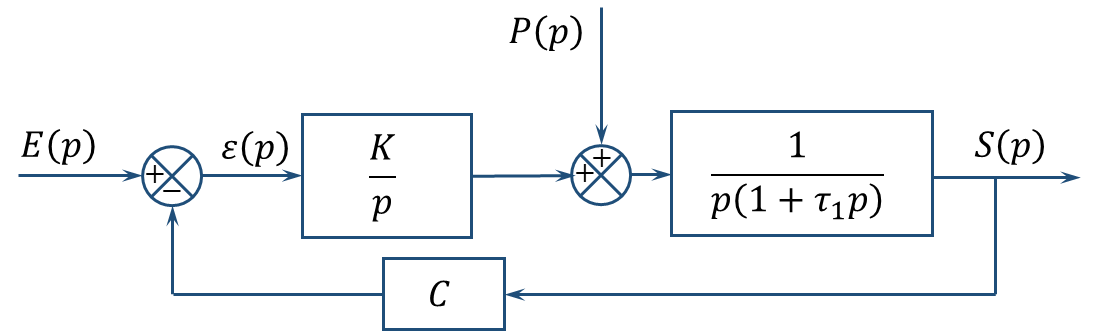
\includegraphics[width=\linewidth]{509_01}
\end{marginfigure}
 \fi
 
\question{Exprimer $\varepsilon(p)$ en fonction de $E(p)$ et $P(p)$.}
\ifprof

On a : 
$\varepsilon(p) = E(p)-C\dfrac{1}{p\left( A+\tau_1 p \right)} \left( \varepsilon(p)\dfrac{K}{p} + P(p)\right)$

$\Leftrightarrow \varepsilon(p) \left(1 +C\dfrac{K}{p^2\left( A+\tau_1 p \right)}\right) = E(p)-C\dfrac{1}{p\left( A+\tau_1 p \right)}  P(p)$

$\Leftrightarrow \varepsilon(p) = E(p)\dfrac{1}{1 +C\dfrac{K}{p^2\left( A+\tau_1 p \right)}}-C\dfrac{1}{p\left( A+\tau_1 p \right)} \dfrac{1}{1 +C\dfrac{K}{p^2\left( A+\tau_1 p \right)}} P(p)$

$\Leftrightarrow \varepsilon(p) = E(p)\dfrac{1}{1 +C\dfrac{K}{p^2\left( A+\tau_1 p \right)}}-\dfrac{C}{p\left( A+\tau_1 p \right) +C\dfrac{K}{p}} P(p)$


\else 
\fi

\question{Évaluer la valeur finale de $\varepsilon(t)$ lorsque $E(p)$ est un échelon d'amplitude $E_0$ et $P(p)$ est un échelon d'amplitude $P_0$.}
\ifprof

On a $\lim\limits_{t\to +\infty} \varepsilon(t) = \lim_{p\to 0} p\varepsilon(p)$.

Dans ces conditons, 
$\varepsilon(p) = E_0\dfrac{1}{p +C\dfrac{K}{p\left( A+\tau_1 p \right)}}-\dfrac{C}{p^2\left( A+\tau_1 p \right) +CK} P_0$.

Au final, $\varepsilon = E_0\dfrac{p}{p +C\dfrac{K}{p\left( A+\tau_1 p \right)}}-\dfrac{Cp}{p^2\left( A+\tau_1 p \right) +CK} P_0$ $=0-0 =0$
\else 
\fi

\question{{Évaluer la valeur finale de $\varepsilon(t)$ lorsque $E(p)$ est un échelon d'amplitude $E_0$ et $P(p)$ est une rampe de pente $P_0$.}
}
\ifprof

Dans ces conditons, 
$\varepsilon(p) = E_0\dfrac{1}{p +C\dfrac{K}{p\left( A+\tau_1 p \right)}}-\dfrac{C}{p^3\left( A+\tau_1 p \right) +CKp} P_0$

et  $\varepsilon = p^2E_0\dfrac{1}{p^2 +C\dfrac{K}{\left( A+\tau_1 p \right)}}-\dfrac{C}{p^2\left( A+\tau_1 p \right) +CK} P_0 = 0 - \dfrac{P_0}{K}=- \dfrac{P_0}{K}$
\else 
\fi

\question{{Évaluer la valeur finale de $\varepsilon(t)$ lorsque $E(p)$ est une rampe de pente $E_0$ et $P(p)$ est un échelon d'amplitude $P_0$.}}
\ifprof

Dans ces conditons, 
$\varepsilon(p) = E_0\dfrac{1}{p^2 +C\dfrac{K}{\left( A+\tau_1 p \right)}}-\dfrac{C}{p^2\left( A+\tau_1 p \right) +CK} P_0$.


On a alors $\varepsilon = pE_0\dfrac{1}{p^2 +C\dfrac{K}{\left( A+\tau_1 p \right)}}-\dfrac{C}{p^2\left( A+\tau_1 p \right) +CK} P_0p = 0$


\else 
\fi

\question{{Évaluer la valeur finale de $\varepsilon(t)$ lorsque $E(p)$ est une rampe de pente $E_0$ et $P(p)$est une rampe de pente  $P_0$.}}
\ifprof

Dans ces conditons, 
$\varepsilon(p) = E_0\dfrac{1}{p^2 +C\dfrac{K}{\left( A+\tau_1 p \right)}}-\dfrac{C}{p^3\left( A+\tau_1 p \right) +CKp} P_0$. 
On a alors
$\varepsilon = E_0 p \dfrac{1}{p^2 +C\dfrac{K}{\left( A+\tau_1 p \right)}}-\dfrac{C}{p^2\left( A+\tau_1 p \right) +CK} p P_0 = -\dfrac{P_0}{K} $.

\else 
\fi




%\question{Réaliser le schéma-blocs.}
%\ifprof
%\begin{figure}[H]
%\centering
%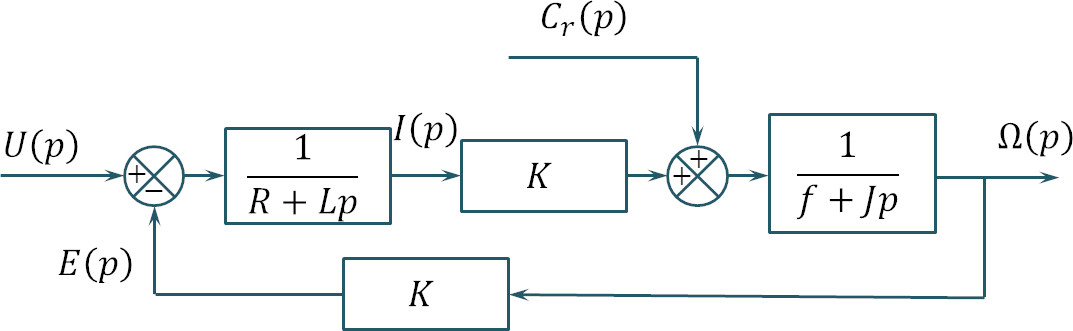
\includegraphics[width=\linewidth]{51_01_c}
%%\caption{Évolution du couple utile en fonction de la vitesse de rotation pour des
%%fréquences de commande de \SI{90}{Hz} à \SI{110}{Hz}. \label{fig_50_04}}
%\end{figure}
%\else
%\fi


 

\ifprof
\else

\marginnote{Corrigé voir \ref{PERF:05:C2:03:509}.}

\fi 
 
\section{Évaluer la précision en utilisant la classe de la BO} 
\graphicspath{{\repStyle/png/}{../PERF/PERF-06-Precision/63_BancHydraulique/images/}} 
\normaltrue \difficilefalse \tdifficilefalse
\correctiontrue
%\UPSTIidClasse{11} % 11 sup, 12 spé
%\newcommand{\UPSTIidClasse}{11}

\exer{Banc hydraulique $\star$ \label{PERF:06:C2:03:prec:63}}
%% CCP MP 2010
\setcounter{question}{0}\marginnote{\xpComp{PERF}{06}}%\UPSTIcompetence[2]{C2-03}
\index{Compétence C2-03}
\index{Schéma-blocs}
\index{Précision}

\ifcorrection
\else
\marginnote{\textbf{Pas de corrigé pour cet exercice.}}
\fi

\ifprof
\else 

Pour limiter l’erreur statique due aux fuites, on envisage d’asservir la pression d’eau dans le tube. 
%L’objectif est ici de proposer un réglage du correcteur pour répondre aux critères du cahier des charges.
La pression d’eau à l’intérieur du tube est mesurée par un capteur de pression. 

\begin{marginfigure}
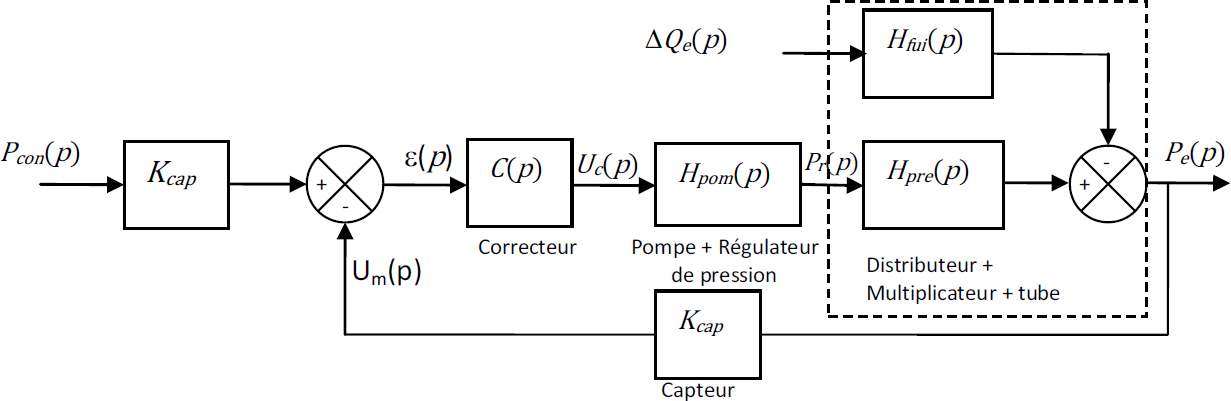
\includegraphics[width=\linewidth]{63_01}
\end{marginfigure}

 
 \begin{tabular}{ll}
$P_{\text{con}}(p)$ : & 	pression de consigne d’eau dans le tube (Pa) \\
$P_e(p)$ : & 	pression d’eau dans le tube (Pa) \\
$U_c(p)$ : & 	tension de commande du régulateur de pression (V)\\
$P_r(p)$ : &	pression d’huile régulée (Pa)\\
$\Delta Q_e(p)$ :& 	débit de fuite (\si{m^3s^{-1}})\\
$U_m(p)$ 	:&	tension de mesure du capteur (V)\\
\end{tabular}
 
 Hypothèses :
\begin{itemize}
\item L’ensemble de mise sous pression {tube + distributeur + multiplicateur de pression} est défini par les transmittances suivantes : $H_{\text{pre}} (p)=\dfrac{K_m}{1+T_1 p}$	et	$H_{\text{fui}} (p)=\dfrac{K_f}{1+T_1 p}$ avec 	$K_m = 3,24$ ; 	$K_f = \SI{2,55e10}{Pa.m^{-3}.s}$ ; 	$T_1  = \SI{10}{s}$.
\item L’ensemble {pompe+régulateur de pression} est modélisé par la fonction de transfert :
$H_{\text{pom}} (p)=\dfrac{K_{\text{pom}}}{1+T_2 p}$  avec 	$K_{\text{pom}} = \SI{1,234e7}{Pa/V}$; 	$T_2 = \SI{5}{s}$.
\item Le capteur est modélisé par un gain pur :	$K_{\text{cap}} = \SI{2,5e-8}{V/Pa}$.
\end{itemize}
La pression de consigne est de $P_{\text{con}} = \SI{800}{bars}$ et les débits de fuite sont estimés à $\Delta Q_e = \SI{5e-4}{m3/s}$.

 
Le cahier des charges concernant le réglage de la pression de test est le suivant.
\begin{center}
\begin{tabular}{lp{8cm}}
\hline 
Stabilité :  & marge de phase de 60\degres  \\
  	  &  marge de gain de \SI{12}{dB} \\ \hline
Rapidité :  &  temps d’établissement te < 40 s \\ \hline
Précision : & 	erreur statique < 5\% soit pour une consigne de 800 bars : \\
&erreur statique due à la consigne : $\varepsilon_{\text{con}}< 5\%$  \\
& erreur statique due à la perturbation $\varepsilon_{\text{pert}} < \SI{40}{bars}$ \\ \hline
Amortissement :&	pas de dépassement \\ \hline
\end{tabular}
\end{center}

Dans le cas d’un système bouclé convenablement amorti, on pourra utiliser, sans aucune justification, la relation :
$t_e \cdot \omega_{\SI{0}{dB}}=3$ où $\omega_{\SI{0}{dB}}$ désigne la pulsation de coupure à \SI{0}{dB} en boucle ouverte et $t_e$ le temps d’établissement en boucle fermée vis-à-vis d’un échelon de consigne :
\begin{itemize}
\item $t_e = t_m$, temps du 1er maximum si le dépassement est supérieur à \SI{5}{\%},
\item $t_e = t_R$, temps de réponse à \SI{5}{\%} si le dépassement est nul ou inférieur à \SI{5}{\%}.
\end{itemize}
On envisage tout d’abord un correcteur de type proportionnel : $C(p)=K_p$. 
\fi

\question{Déterminer, en fonction de $K_p$ ,  $\varepsilon_{\text{con}}$ définie comme l’erreur statique pour une entrée consigne $P_{\text{con}}$ de type échelon, dans le cas où le débit de fuite est nul.}
\ifprof

Le débit de fuite est nul; donc $\Delta Q_e(p)=0$.

\textbf{Cas 1 : cours sur la précision connu \textit{-- Attention à avoir le même type d'entrée/sortie}}

La FTBO est de classe nulle ($C(p)$ est un gain, $H_{\text{pom}} (p)$ et $H_{\text{pre}} (p)$ de classe 0). Le gain de la Boucle ouverte est $K_{\text{BO}}=K_p K_m K_{\text{pom}}K_{\text{cap}}$.


Si l'entrée est un échelon d'amplitude $P_0$, l'écart statique est donc donné par 
$\varepsilon_S = \dfrac{P_0}{1+K_{\text{BO}}}= \dfrac{P_0}{1+K_p K_m K_{\text{pom}}K_{\text{cap}}}$.



\textbf{Cas 2 : cours sur la précision peu connu -- À savoir faire, mais on perd un peu de temps... \textit{-- Attention à avoir le même type d'entrée/sortie}}
Si on connait quand même un petit peu son cours, on a 
$\varepsilon(p)
=
\dfrac{P_{\text{con}}(p)}%
{1+K_P \dfrac{K_{\text{pom}}}{1+T_2 p} \dfrac{K_m}{1+T_1 p} K_{\text{cap}}}$.

On a alors,
$\varepsilon_s = \lim\limits_{p\to 0} p 
\dfrac{\dfrac{P_0}{p}}%
{1+K_P \dfrac{K_{\text{pom}}}{1+T_2 p} \dfrac{K_m}{1+T_1 p} K_{\text{cap}}}$
$=
\dfrac{P_0}%
{1+K_P K_{\text{pom}}K_m K_{\text{cap}}}
$

\textbf{Cas 3 : cours sur la précision pas connu -- À savoir faire, mais on perd beaucoup peu de temps...}

En utilisant la formule de Black, on a $P_e(p) 
= P_{\text{con}}(p) K_{\text{cap}} 
\dfrac{K_P \dfrac{K_{\text{pom}}}{1+T_2 p} \dfrac{K_m}{1+T_1 p} }%
{1+K_P \dfrac{K_{\text{pom}}}{1+T_2 p} \dfrac{K_m}{1+T_1 p} K_{\text{cap}}}$

$= P_{\text{con}}(p) K_{\text{cap}}(p) 
\dfrac{K_P K_{\text{pom}}K_m }%
{\left(1+T_2 p\right)\left(1+T_1 p\right)+K_P K_{\text{pom}} K_m K_{\text{cap}}}$

En passant à la valeur finale avec une entrée échelon, on a 
$\lim\limits_{t\to +\infty}P_e(t)$ $ =  P_{0} K_{\text{cap}} 
\dfrac{K_P K_{\text{pom}}K_m }%
{1+K_P K_{\text{pom}} K_m K_{\text{cap}}}$

L'écart statique est donc donné par
$
\varepsilon_S = P_0 - P_{0} 
\dfrac{K_P K_{\text{pom}}K_m K_{\text{cap}} }%
{1+K_P K_{\text{pom}} K_m K_{\text{cap}}}$
$= P_0
\dfrac{1+K_P K_{\text{pom}} K_m K_{\text{cap}} - K_P K_{\text{pom}}K_m K_{\text{cap}} }{1+K_P K_{\text{pom}} K_m K_{\text{cap}}}
$

$= 
\dfrac{P_0}{1+K_P K_{\text{pom}} K_m K_{\text{cap}}}$

\else 
\fi

\question{Proposer un réglage de $K_p$ pour limiter $\varepsilon_{\text{con}}$ à la valeur spécifiée dans le cahier des charges.}
\ifprof
On souhaite que l'écart statique soit inférieure à 5\% soit 0,05 pour une entrée unitaire. 

On cherche donc $K_P$ tel que 
$\dfrac{1}{1+K_P K_{\text{pom}} K_m K_{\text{cap}}}<0,05 $
$ \Leftrightarrow 1<0,05\left(1+K_P K_{\text{pom}} K_m K_{\text{cap}}\right)$

$ \Leftrightarrow \dfrac{1 - 0,05}{0,05 K_{\text{pom}} K_m K_{\text{cap}}}<K_P $

Soit $ K_P > \dfrac{1 - 0,05}{0,05 \times 1,234 \times 10^7\times 3,24 \times  2,5 \times 10^{-8}}  \Rightarrow K_P > 19$.
\else 
\fi

\question{Dans le cas où la consigne de pression est nulle,  déterminer en fonction de $K_p$ la fonction de transfert en régulation définie par : $H_{\text{pert}}(p)=\dfrac{P_e (p)}{\Delta Q_e (p)}$. En déduire, en fonction de $K_p$,  $\varepsilon_{\text{pert}}$  définie comme l’erreur statique pour une perturbation $\Delta Q_e$ de type échelon, dans le cas où la consigne de pression est nulle.}
\ifprof
Dans ce cas il n'y a pas d'intégrateur avant la perturbation échelon. Il faut savoir faire le calcul.

On peut utiliser la << lecture directe >> :
$P_e(p)= P_r(p)\indice{H}{pre} - \Delta Q_e(p) \indice{H}{fui}(p)$

$= \indice{H}{pre}(p)\indice{H}{pom}(p) C(p) \varepsilon(p)- \Delta Q_e(p) \indice{H}{fui}(p)$

$= -\indice{H}{pre}(p)\indice{H}{pom}(p) C(p) \indice{K}{cap} P_e(p)- \Delta Q_e(p) \indice{H}{fui}(p)$.

$\Leftrightarrow P_e(p) \left(1+\indice{H}{pre}(p)\indice{H}{pom}(p) C(p) \indice{K}{cap} \right)
=- \Delta Q_e(p) \indice{H}{fui}(p)$

$\Leftrightarrow \dfrac{P_e(p)}{\Delta Q_e(p)} 
=-  \dfrac{\indice{H}{fui}(p)}{1+\indice{H}{pre}(p)\indice{H}{pom}(p) C(p) \indice{K}{cap}}$


Calculons $\indice{\varepsilon}{pert}(p) = -  \dfrac{\indice{H}{fui}(p)}{1+\indice{H}{pre}(p)\indice{H}{pom}(p) C(p) \indice{K}{cap}} \Delta Q_e(p) \indice{K}{cap}$.

On a alors $\indice{\varepsilon}{pert}= \tvf{\varepsilon}$ 
$= \lim\limits_{p\to 0} - p\times  \dfrac{\indice{H}{fui}(p)}{1+\indice{H}{pre}(p)\indice{H}{pom}(p) C(p) \indice{K}{cap}} \dfrac{\Delta Q_0}{p} \indice{K}{cap}$

$= - \dfrac{K_f\Delta Q_0 \indice{K}{cap}}{1+K_m\indice{K}{pom} K_P \indice{K}{cap}} $

\else 
\fi

\question{Proposer un réglage de $K_p$ pour limiter $\varepsilon_{\text{pert}}$ à la valeur spécifiée au cahier des charges.}
\ifprof
Pour $\Delta Q_e = \SI{5e-4}{m^3.s^{-1}}$, il faut $\indice{\varepsilon}{pert}<40\times 10^5$ (Pa) soit

$\dfrac{K_f\Delta Q_0 \indice{K}{cap} }{1+K_m\indice{K}{pom} K_P \indice{K}{cap}}  < 40\times 10^5$
$\Rightarrow  K_f\Delta Q_0 \indice{K}{cap}  < 40\times 10^5\left(1+K_m\indice{K}{pom} K_P \indice{K}{cap}\right)$
$\Rightarrow \dfrac{K_f\Delta Q_0 \indice{K}{cap}  -40\times 10^5}{40\times 10^5 K_m\indice{K}{pom} \indice{K}{cap} }< K_P $
$\Rightarrow K_P > -1$
\else 
\fi

\question{Proposer un réglage de $K_p$ pour vérifier le critère d’amortissement. Conclure quant au choix d’un correcteur proportionnel.}
\ifprof
Je vous laisse faire le calcul... Il faut savoir le faire le plus vite possible.
Il faut d'abord calculer la FTBF, la mettre sous forme canonique, déterminer 
$\indice{\xi}{BF}=\dfrac{T_1+T_2}{2\sqrt{T_1T\left( 1+K_P K_M \indice{K}{Pom}\indice{K}{Cap}\right)}}$ puis
determiner $K_P$ tel que $\indice{\xi}{BF}=1$.

\else 
\fi
 

\ifprof
\else
\begin{solution}
\begin{enumerate}
  \item $\varepsilon_{\text{con \%}} = \dfrac{1}{1+K_PK_m K_{\text{pom}} K_{\text{cap}} }$;
  \item $K_P > 19$;
  \item $\varepsilon_{\text{pert}} = \Delta Q_e \dfrac{K_f}{1+K_{\text{cap}}K_PK_mK_{\text{pom}}}$;
  \item $K_P > -1$.% $K_P > 2,19$.
  \item $K_P < 0,125$. Il est impossible de vérifier les trois conditions avec un correcteur proportionnel.
\end{enumerate}
\end{solution}

\marginnote{Corrigé voir \ref{PERF:06:C2:03:prec:63}.}

\fi 
 
\graphicspath{{\repStyle/png/}{../PERF/PERF-06-Precision/64_EPAS/images/}} 
\normaltrue \difficilefalse \tdifficilefalse
\correctionfalse
%\UPSTIidClasse{11} % 11 sup, 12 spé
%\newcommand{\UPSTIidClasse}{11}

\exer{Exercice $\star$ \label{PERF:06:C2:03:prec:64}}
%% CCP MP 2007
\setcounter{question}{0}\marginnote{\xpComp{PERF}{06}}%\UPSTIcompetence[2]{C2-03}
\index{Compétence C2-03}
\index{Schéma-blocs}
\index{Précision}

\ifcorrection
\else
\marginnote{\textbf{Pas de corrigé pour cet exercice.}}
\fi


\ifprof
\else
On donne le système suivant dont la la FTBF est donnée par 
$G(p)=\dfrac{\Theta_S(p)}{\Theta_C(p)}=\dfrac{3,24}{p^2+3,24 p+3,24}$. Le retard du système est de \SI{0,2}{s}.

L'asservissement est donné par le schéma-blocs suivant.

\begin{marginfigure}
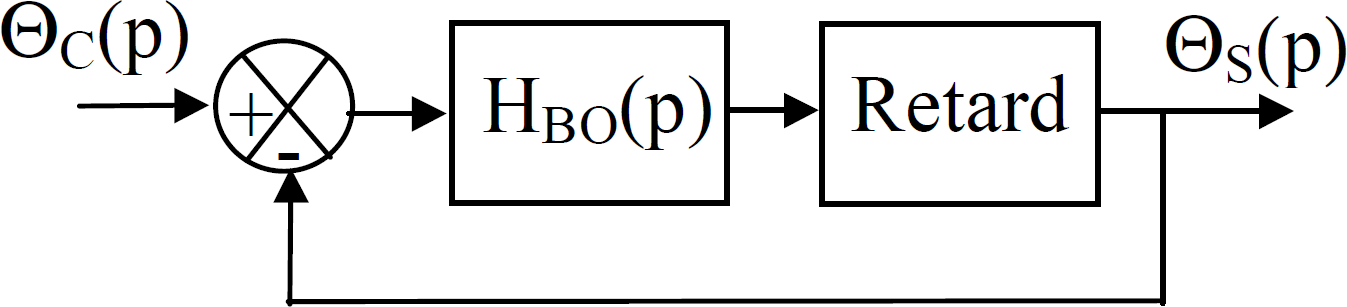
\includegraphics[width=\linewidth]{64_01}
\end{marginfigure}

\fi

 
\question{En considérant le retard nul, déterminer l'écart statique.}
\ifprof
\else 
\fi

\question{En considérant le retard nul, déterminer l'écart statique, déterminer l'expression de la boucle ouverte $H_{\text{BO}}(p)$.}
\ifprof
\else 
\fi
 
\question{Déterminer l'expression de $G_r(p)$, transmittance en boucle fermée du système avec retard de \SI{0,2}{s}.}
\ifprof
\else 
\fi
Le système est soumise à une rampe de \SI{0,1}{rad.s^{-1}}.
 
\question{Donner la valeur de l’erreur de traînage correspondant à cette entrée, en
négligeant le retard.}
\ifprof
\else 
\fi
 
\question{Donner la valeur de l'écart statique du système avec retard.}
\ifprof
\else 
\fi
 
\question{Donner la valeur de l'erreur de traînage du système avec retard.}
\ifprof
\else 
\fi

\ifprof
\else

\noindent\footnotesize
% \fbox{\parbox{.9\linewidth}{
% Éléments de corrigé : 
% \begin{enumerate}
  % \item $\varepsilon_{\text{con \%}} = \dfrac{1}{1+K_PK_m K_{\text{pom}} K_{\text{cap}} }$;
  % \item $K_P > 19$;
  % \item $\varepsilon_{\text{pert}} = \Delta Q_e \dfrac{K_f}{1+K_{\text{cap}}K_PK_mK_{\text{pom}}}$;
  % \item $K_P > 2,19$.
  % \item $K_P < 0,125$. Il est impossible de vérifier les trois conditions avec un correcteur proportionnel.
% \end{enumerate}}}
\normalsize


\marginnote{Corrigé voir \ref{PERF:06:C2:03:prec:64}.}

\fi 
 
\graphicspath{{\repStyle/png/}{../PERF/PERF-06-Precision/73_Bassin/images/}} 
\normaltrue \difficilefalse \tdifficilefalse
\correctionfalse
%\UPSTIidClasse{11} % 11 sup, 12 spé
%\newcommand{\UPSTIidClasse}{11}

\exer{Exercice $\star$ \label{PERF:06:C2:03:prec:73}}
%% CCP MP 2007
\setcounter{question}{0}\marginnote{\xpComp{PERF}{06}}%\UPSTIcompetence[2]{C2-03}
\index{Compétence C2-03}
\index{Schéma-blocs}
\index{Précision}

\ifcorrection
\else
\marginnote{\textbf{Pas de corrigé pour cet exercice.}}
\fi


\ifprof
\else
L'asservissement de vitesse est à présent modélisé par le schéma-blocs de la figure suivante à retour unitaire. Cet asservissement n’est valable que pour les petites variations de vitesse. $H(p)$ correspond à la fonction de transfert en boucle ouverte naturelle (non corrigée), $C(p)$ est le correcteur.

\begin{marginfigure}
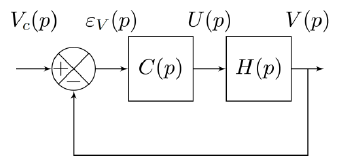
\includegraphics[width=\linewidth]{73_01}
\end{marginfigure}

 $H(p)=\dfrac{K_N}{(1+T_m p)(1+T_e p)}$ avec $K_N = \SI{20}{ms.^{-1}V^{-1}}$, $T_m = \SI{5}{s}$, $T_e = \SI{0,5}{s}$.
 
 \begin{obj}
\begin{itemize}
\item  Exigence 1.2 : Garantir un déplacement du chariot de vitesse : 
\begin{itemize}
\item  1.2.3 Précision :
\begin{itemize}
\item Erreur statique pour une entrée $v_c(t)=V_0 u(t)$ avec $V_0 = \SI{8}{m.s^{-1}}$ : $E_S = \SI{0}{m.s^{-1}}$.
\item Erreur de trainage pour une entrée $v_c(t)=\gamma_0 t  u(t)$ avec $\gamma_0 = \SI{1,6}{m.s^{-2}}$ : $E_T \leq   \SI{0,16}{m.s^{-1}}$.
\end{itemize}
\end{itemize}
\end{itemize}
 \end{obj}
 Le concepteur choisit un correcteur Proportionnel Intégral : $C_1(p)=\dfrac{C}{T_i p} \left(1+T_i p\right)$ avec $T_i = T_m$.
 
\fi
 
 
\question{Déterminer les expressions littérales de l'erreur statique $E_S$ (consigne : échelon d'amplitude $V_0$) et de l'erreur de trainage $E_T$ (consigne : rampe de pente $\gamma_0$) de cet asservissement corrigé avec $C_1(p)$ en fonction de la consigne, du gain $K_N$ et des paramètres du correcteur et $C$  et $T_m$.}
\ifprof
\else 
\fi

\question{ En déduire la condition (notée $C_{\varepsilon}$) sur le gain $C$ du correcteur permettant de satisfaire l’exigence 1.2.3 du cahier des charges.}
\ifprof
\else 
\fi

On choisit finalement un correcteur PID : $C_2(p)=C\left(1+\dfrac{1}{T_i p}+T_d p \right)$ avec $T_i = 2 T_e$ et $T_d = \dfrac{T_e}{2}$.

\question{Montrer qu'on peut mettre ce correcteur sous la forme  $C_2(p)= \dfrac{K}{p}\left(1+Tp\right)^2$ et donner les expressions de $K$  et de $T$ en fonction de $C$ et $T_e$.}
\ifprof
\else 
\fi


\question{Donner l'expression de la fonction de transfert en boucle ouverte du système corrigé.}
\ifprof
\else 
\fi

\question{Déterminer les expressions littérales de l'erreur statique $E_S$ (consigne : échelon d'amplitude $V_0$) et de l'erreur de traînage $E_T$ (consigne : rampe de pente $\gamma_0$) de cet asservissement corrigé.}
\ifprof
\else 
\fi

\question{ En déduire la condition sur la valeur du gain $K$ du correcteur permettant de satisfaire l’exigence 1.2.3 du cahier des charges.}
\ifprof
\else 
\fi

\ifprof
\else


\marginnote{Corrigé voir \ref{PERF:06:C2:03:prec:73}.}

\fi 
 

\proftrue
\setcounter{chapter}{0}
\setchapterpreamble[u]{\margintoc} 
\chapter{Évaluer les performances d'un SLCI} 
\section{Évaluer la stabilité en utilisant la BF, les pôles de la BF} 
\section{Évaluer la stabilité en utilisant les marges de la BO} 
\graphicspath{{\repStyle/png/}{../PERF/PERF-02-Marges/61_Hemostase/images/}} 
\normaltrue \difficilefalse \tdifficilefalse
\correctionfalse
%\UPSTIidClasse{11} % 11 sup, 12 spé
%\newcommand{\UPSTIidClasse}{11}

\exer{Hemostase -- Stabilité$\star$ \label{PERF:02:C2:03:stab:61}}

\setcounter{question}{0}\marginnote{\xpComp{PERF}{02}}%\index{Compétence C2-03}\index{Compétence PERF-02}
\index{Compétence C2-03}
\index{Schéma-blocs}
\index{Stabilité}

%%%%%%%%%%%%%%%%%%%%%%%%%%%%%%%


\ifprof
\else
La modélisation de l'asservissement de position est donnée par le schéma-bloc ci-dessous dans lequel $K_2 = 2,78 \cdot 10^{-2} \text{N}^{-1}$, $K_1 = \SI{856}{s^{-1}}$, $T_m= 3\cdot  10^{-2} s$.

Le couple résistant $C_r$ est constant et vaut $C_{r0} = 2,7 \cdot 10^{-3} \text{Nm}$.


\begin{marginfigure}
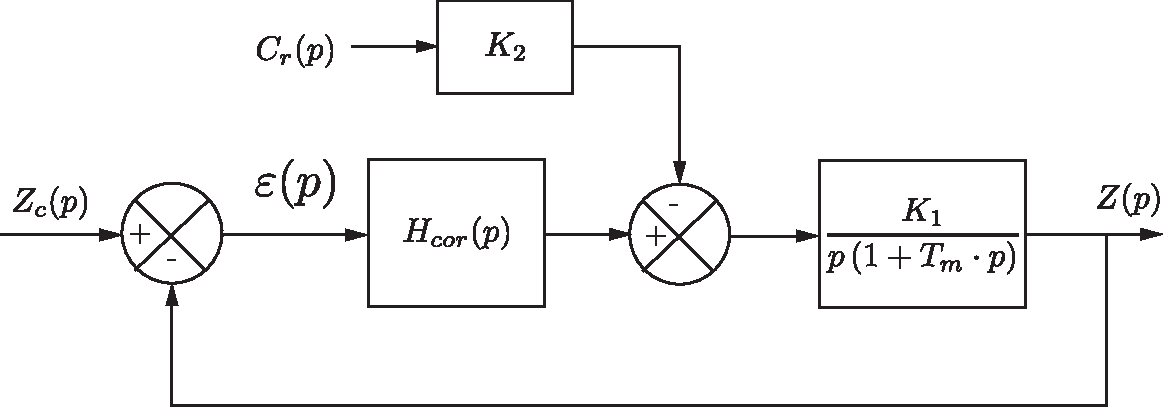
\includegraphics[width=\linewidth]{64_01.pdf}
\end{marginfigure}

On suppose le correcteur proportionnel : $H_{\text{cor}}(p)=K_p$.

Les performances du système sont détaillées dans le diagramme des exigences partiel.% (figure \ref{req}). 


\begin{marginfigure}
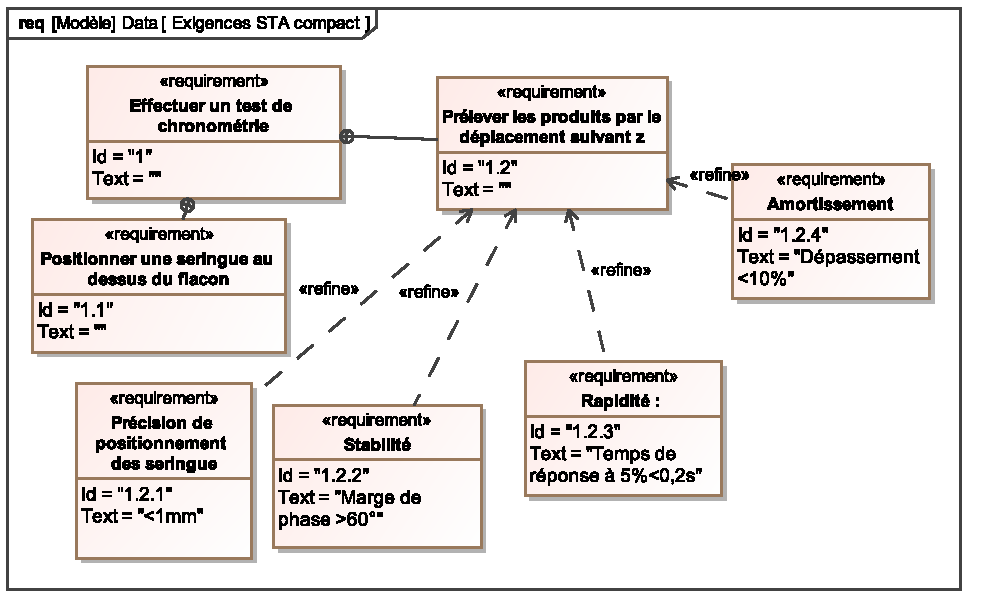
\includegraphics[width=\linewidth]{req.pdf}
\end{marginfigure}



\fi
\question{Déterminer l'expression de la fonction de transfert en boucle ouverte $H_{\text{bo}}(p)=\left(\frac{Z(p)}{\varepsilon(p)}\right)_{C_r(p)=0}$ ainsi que la fonction de transfert $H_{\text{cr}}(p)=\left(\frac{Z(p)}{C_r(p)}\right)_{Z_c=0}$.}
\ifprof
%\begin{corrige}~\\

$H_{\text{bo}}(p) = H_{\text{cor}}(p) \dfrac{K_1}{p\left(1+T_m p\right)}$ $=  \dfrac{K_1 K_p}{p\left(1+T_m p\right)}$.

$H_{\text{cr}}(p)= -K_2\dfrac{\dfrac{K_1}{p\left(1+T_m p\right)}}{1+H_{\text{cor}}(p) \dfrac{K_1}{p\left(1+T_m p\right)}}$

$= -K_2\dfrac{K_1}{p\left(1+T_m p\right)+H_{\text{cor}}(p) K_1}$
$= -\dfrac{K_1K_2}{p\left(1+T_m p\right)+K_p K_1}$
%\end{corrige}
\else
\fi

\question{Déterminer l'erreur statique pour une entrée de type échelon d'amplitude $Z_{c0}$ dans l'hypothèse d'une perturbation nulle ($C_{r0}$). Déterminer ensuite l'erreur due à une perturbation constante $C_{r0}$, dans le cas d'une
consigne de position nulle ($Z_c=0$). En déduire la valeur de $K_p$ pour satisfaire le critère de précision du cahier des charges.}
\ifprof
%\begin{corrige}
Exprimons $\varepsilon(p)$ en fonction de $Z_c(p)$ et $C_{r}(p)$ :

$
\varepsilon(p)=Z_c(p)-Z(p) = Z_c(p)- \left(\varepsilon(p) H_{\text{cor}}(p)-   K_2 C_r(p)\right) \dfrac{K_1}{p\left(1+T_m p\right)}$

$\Leftrightarrow \varepsilon(p)\left(1 +  H_{\text{cor}}(p)\dfrac{K_1}{p\left(1+T_m p\right)} \right) 
= Z_c(p) + K_2 C_r(p) \dfrac{K_1}{p\left(1+T_m p\right)}$

$\Leftrightarrow \varepsilon(p)  = 
Z_c(p)\dfrac{1}{1 +  H_{\text{cor}}(p)\dfrac{K_1}{p\left(1+T_m p\right)}} 
+   K_2 C_r(p) \dfrac{K_1}{p\left(1+T_m p\right)} \dfrac{1}{1 +  H_{\text{cor}}(p)\dfrac{K_1}{p\left(1+T_m p\right)}}$

$\Leftrightarrow \varepsilon(p)  = 
Z_c(p)\dfrac{{p\left(1+T_m p\right)}}{{p\left(1+T_m p\right)} +  H_{\text{cor}}(p){K_1}} 
+  K_2 C_r(p)  \dfrac{K_1}{p\left(1+T_m p\right) +  H_{\text{cor}}(p){K_1}}$


En prenant une entrée échelon et une perturbation échelons, on a $Z_c(p) = \dfrac{Z_{c0}}{p}$ et 
$C_{r}(p) = \dfrac{C_{r0}}{p}$.

On a donc $\lim\limits_{t\to +\infty} \varepsilon(t) $
$=\lim\limits_{p\to 0} p\varepsilon(p)$
$=  \lim\limits_{p\to 0} Z_{c0}\dfrac{{p\left(1+T_m p\right)}}{{p\left(1+T_m p\right)} +  H_{\text{cor}}(p){K_1}} 
+   K_2 C_{r0}  \dfrac{K_1}{p\left(1+T_m p\right) +  H_{\text{cor}}(p){K_1}} $ 
$ =   \dfrac{K_2 C_{r0}}{ K_p}$.

AN : $\varepsilon_s < \SI{1}{mm}$
$\Leftrightarrow \dfrac{K_2 C_{r0}}{ K_p} < \SI{1}{mm}$  
$\Leftrightarrow 
2,78 \cdot 10^{-2} \times 2,7 \cdot 10^{-3} \times 10^3<  K_p$  soit $K_p >0,08$.
%\end{corrige}
\else
\fi


\question{Sur le document réponse %de la figure (\ref{bode_bo}) 
compléter les diagrammes de Bode en gain et en phase de $H_{\text{bo}}(p)$ pour $K_p$ déterminé précédemment. Indiquer si le critère de stabilité est satisfait en justifiant votre démarche par des tracés nécessaires.}
\ifprof
%\begin{corrige}~\\
En ajoutant le gain de 0,08, il faut translater la courbe de gain vers le bas de 22 dB.

\begin{marginfigure}
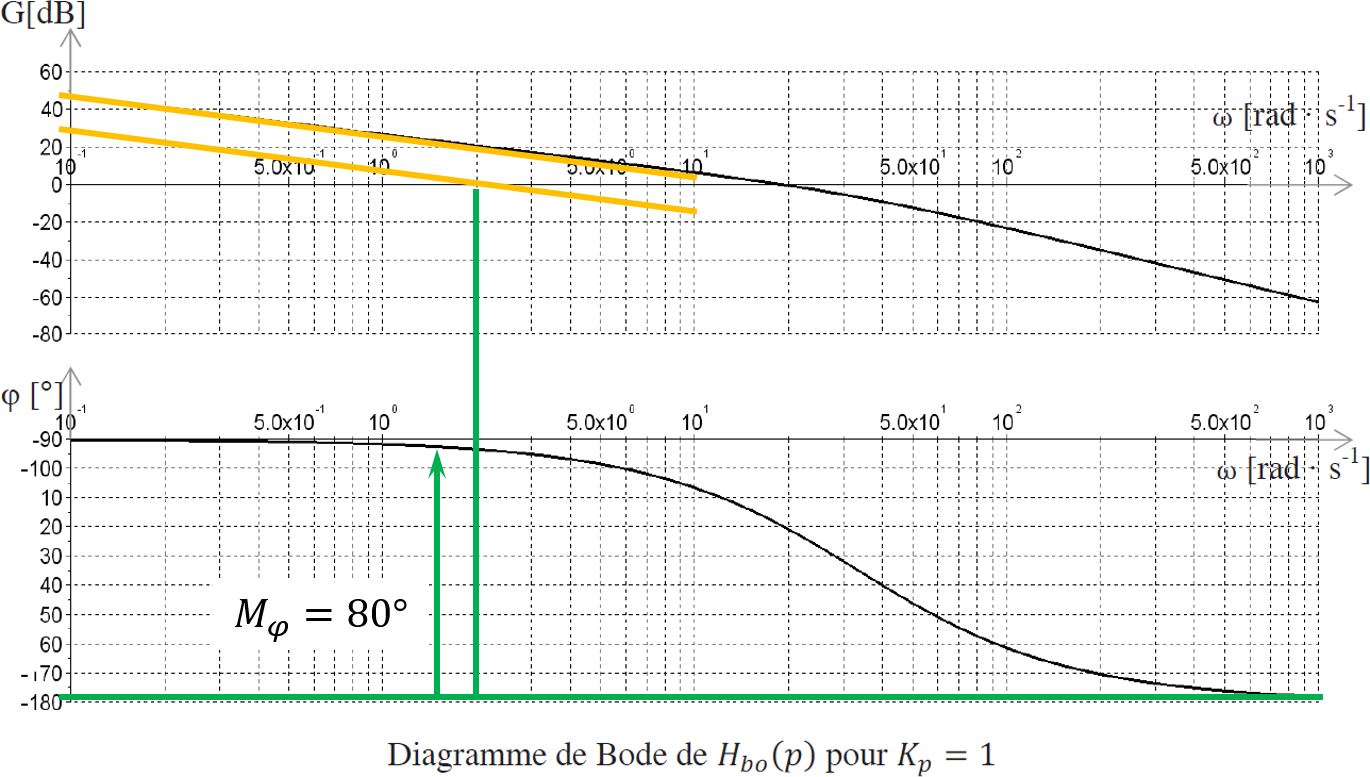
\includegraphics[width=\linewidth]{cor_06}
\end{marginfigure}

La marge de phase est supérieure à 60\degres.
%\end{corrige}
\else
\fi

Afin d'améliorer le comportement, on implante un correcteur Proportionnel Intégral ayant pour fonction de transfert : $H_{\text{cor}}(p)=\frac{K_p\left(1+T_i\cdot p\right)}{T_i\cdot p}$ avec $K_p=1$ et $T_i = \SI{1}{s}$.

\question{Tracer le diagramme de Bode de la fonction de transfert en boucle ouverte avec ce correcteur avec $K_p=1$ et $T_i = \SI{1}{s}$.}% sur la figure \ref{bode_bo_PI}.}
\ifprof
%\begin{corrige}
%\end{corrige}
\else
\fi

\question{On souhaite une marge de phase d'au moins $60^{\circ}$. Proposer un réglage de $K_p$ pour satisfaire au cahier des charges.}% Justifier vos calculs par les tracés nécessaires sur la figure \ref{bode_bo_PI}.}
\ifprof
%\begin{corrige}
%\end{corrige}
\else
\fi

\question{La figure suivante %\ref{reponse_2nd_ordre} 
donne la réponse à un échelon de position de \SI{50}{mm} avec trois types de correcteurs. Vérifier qu'elle est conforme au cahier des charges. Justifier clairement vos réponses en donnant les valeurs numériques pour chaque critère.}
\ifprof

%\begin{corrige} ~\\
\begin{center}
\begin{tabular}{|l|c|c|c|}
\hline
 & P & PI & PID \\  \hline
 Temps de réponse < à 5\,\% < \SI{0,2}{s} &Ok & Ok & Ok \\ \hline
Précision < \SI{1}{mm} & Ok (?) & Ok & Ok \\ \hline
 Dépassement < à 10\,\% < \SI{0,2}{s} & Pas Ok & Pas Ok & Ok \\ \hline
\end{tabular}
\end{center}

\begin{marginfigure}
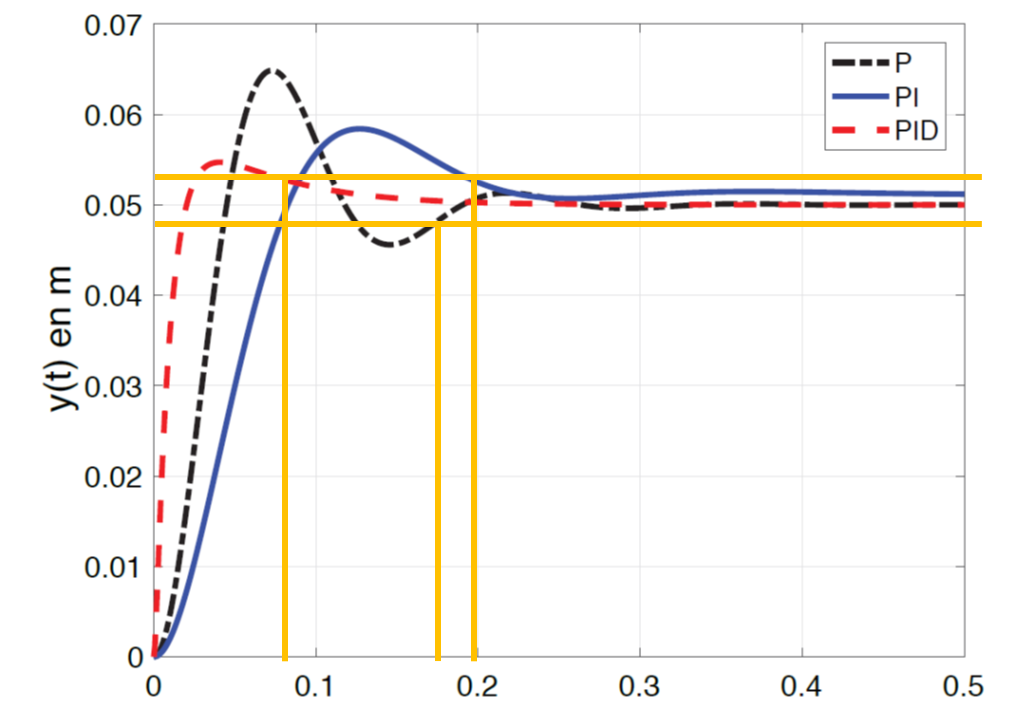
\includegraphics[width=\linewidth]{cor_07}
\end{marginfigure}

%\end{corrige}
\else
\fi

\ifprof
\else
%\begin{figure}[!htb]
\begin{marginfigure}
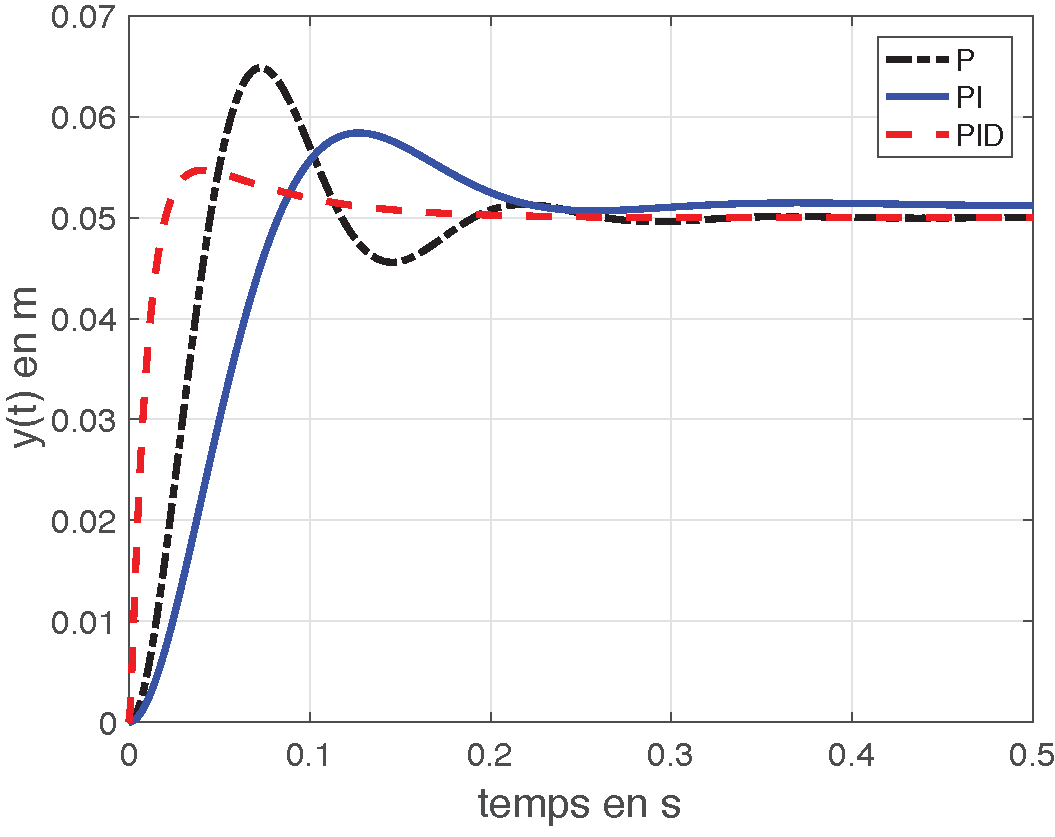
\includegraphics[width=\linewidth]{64_02}
%\caption{Réponse à un échelon de position de $50 mm$ avec trois correcteurs P(question 2) PI (question 5) et PID (déterminé numériquement)\label{reponse_2nd_ordre}}
\end{marginfigure}
%\end{figure}
\fi

\question{Analyser les résultats à l'aide du diagramme de Bode de la FTBO corrigé avec un PID optimisé.}% (figure \ref{bode_pid}.)}
\ifprof
%\begin{corrige}~\\

\begin{marginfigure}
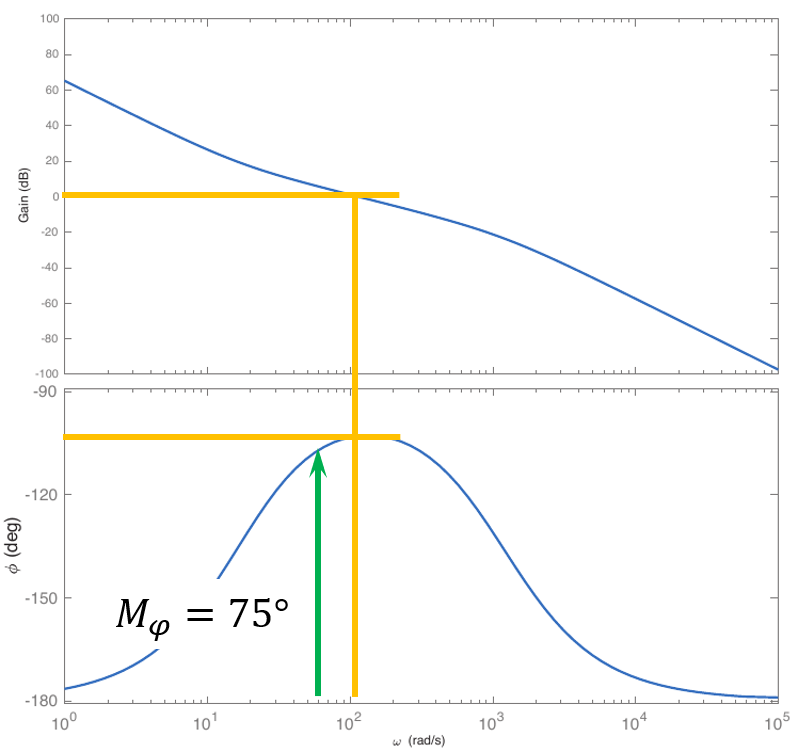
\includegraphics[width=\linewidth]{cor_08}
\end{marginfigure}

La marge de phase est supérieure à 60\degres.

%\end{corrige}
\else
\fi


\ifprof
\else
\begin{marginfigure}
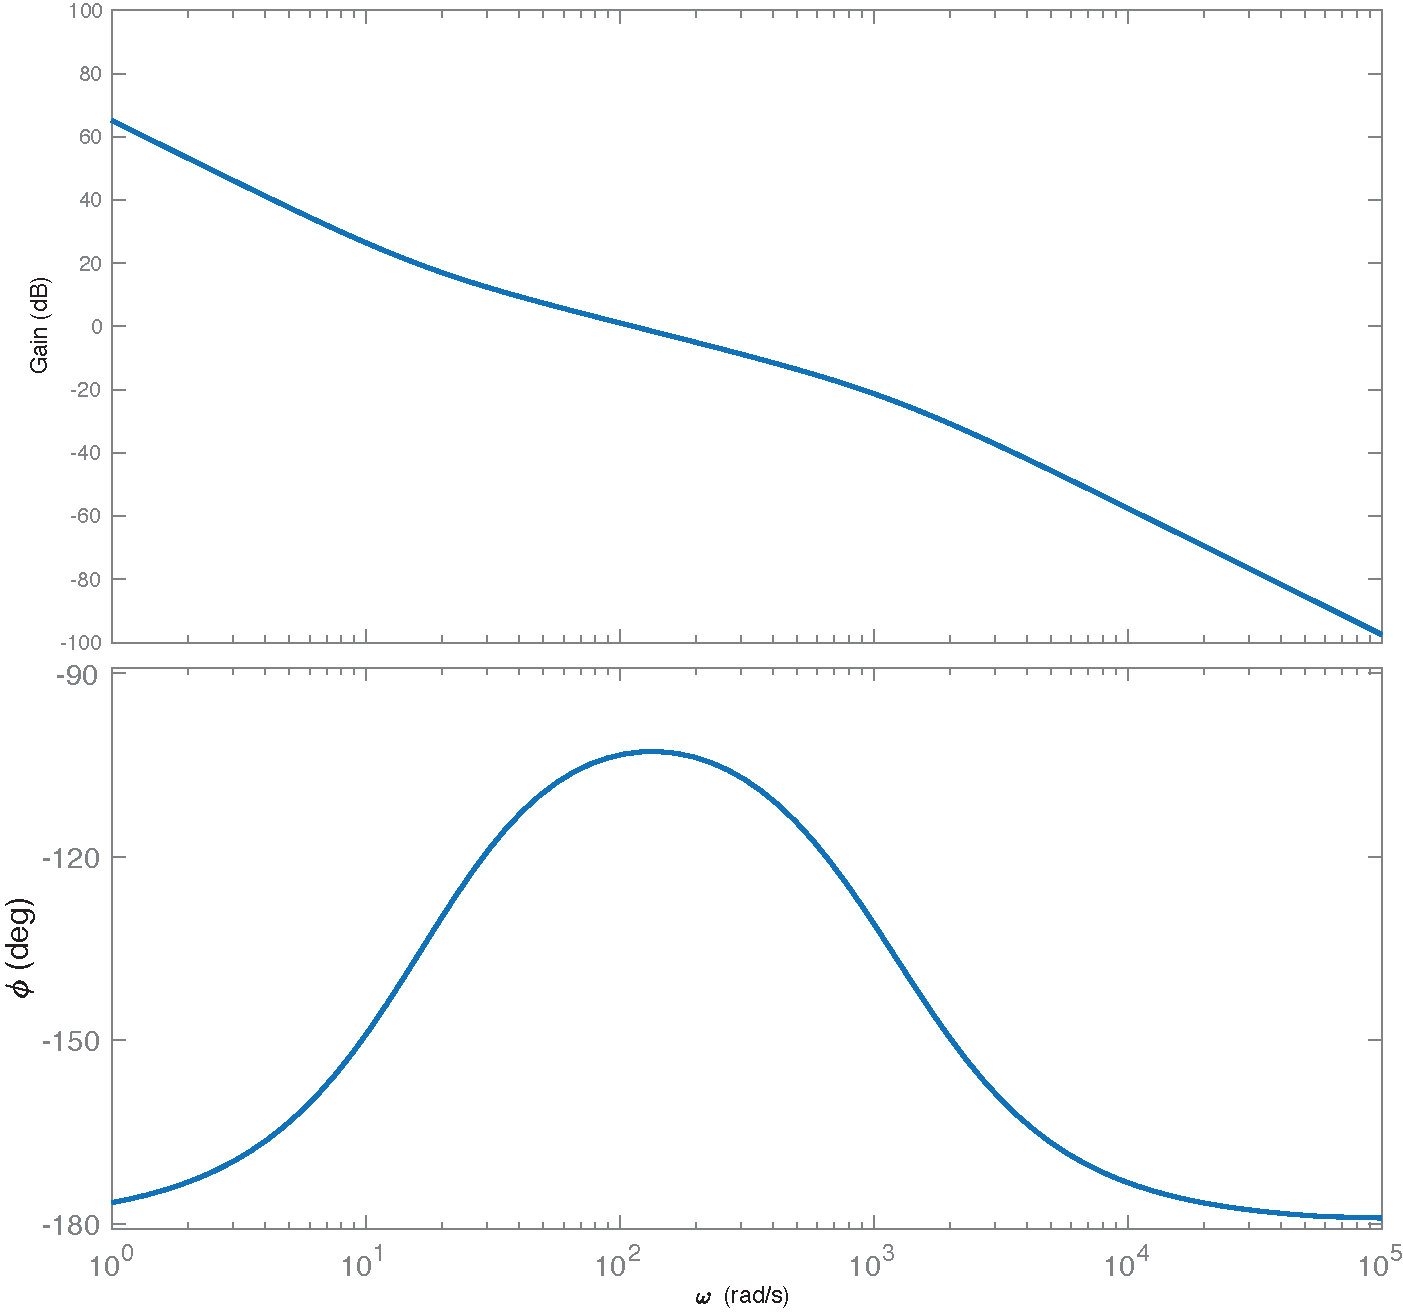
\includegraphics[width=\linewidth]{64_03}
%\caption{Diagramme de Bode de $H_{bo}(p)$ avec un correcteur PID pour $K_p=0,19$, $K_i=2,1$ et $K_d=0,0038$\label{bode_pid}}
\end{marginfigure}
\fi


%%%%%%%%%%%%%%%%%%%%%%%%%%%%%%%
 

\ifprof
\else
%
%\noindent\footnotesize
%\fbox{\parbox{.9\linewidth}{
%Éléments de corrigé : 
%\begin{enumerate}
%  \item $k_{BO}=\sqrt{2}{\tau_m}$.
%    \item $k_c=\dfrac{\sqrt{2}N}{\tau_m k_m k_r} = 471,1$.
%    \item $\varepsilon_s=0$.
%\end{enumerate}}}
%\normalsize


\marginnote{Corrigé voir \ref{PERF:02:C2:03:stab:61}.}

\fi 
 
\graphicspath{{\repStyle/png/}{../PERF/PERF-02-Marges/62_Palettisation/images/}} 
\normaltrue \difficilefalse \tdifficilefalse
\correctiontrue
%\UPSTIidClasse{11} % 11 sup, 12 spé
%\newcommand{\UPSTIidClasse}{11}

\exer{Palettisation -- Stabilité $\star$ \label{PERF:02:C2:03:stab:62}}
%% CCP MP 2010
\setcounter{question}{0}\marginnote{\xpComp{PERF}{02}}%\index{Compétence C2-03}\index{Compétence PERF-02}
\index{Compétence C2-03}
\index{Schéma-blocs}
\index{Stabilité}

\ifcorrection
\else
\marginnote{\textbf{Pas de corrigé pour cet exercice.}}
\fi


\ifprof 
\else
Une boucle de position est représentée ci-dessous. On admet que :  
\begin{itemize}
\item $H(p)=\dfrac{\Omega_m(p)}{U_v(p)}=\dfrac{30}{1+\num{5e-3}p}$;
\item $K_r = \SI{4}{V.rad^{-1}}$ : gain du capteur de position;
\item $K_a$ : gain de l’adaptateur du signal de consigne $\alpha_e(t)$; 
\item $N=200$ : rapport de transmission du réducteur (la réduction est donc de $1/N$).
\item le signal de consigne $\alpha_e(t)$ est exprimé en degré ; 
\item le correcteur $C(p)$ est à action proportionnelle de gain réglable $K_c$. 
\end{itemize}


\begin{center}
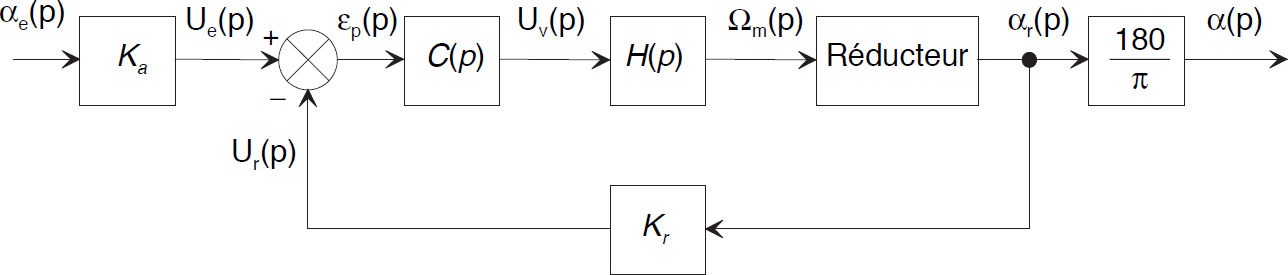
\includegraphics[width=\linewidth]{62_01}
\end{center}
 \fi
 
 
 On montre que la fonction de transfert du réducteur est $R(p)=\dfrac{\alpha_r(p)}{\Omega_m(p)}=\dfrac{1}{Np}$, que  $k_a=\dfrac{\pi}{180}k_r$ et que la FTBO est donnée par $T(p)=\dfrac{k_{BO}}{p\left(1+\tau_m p\right)}$ ($k_{BO}=\dfrac{k_c k_m k_r}{N}$).
 
 
 On souhaite une marge de phase de 45\degres.
 
\question{Déterminer la valeur de $K_{BO}$ permettant de satisfaire cette condition.}
\ifprof
On souhaite une marge de phase de 45\degres. On cherche donc $\omega_{\varphi}$ tel que 
$\varphi\left(\omega_{\varphi}\right)=-180+45 = -135\degres$.

$\varphi(\omega)=-90-\arg\left(1+\tau_m j \omega \right) =-90-\arctan\left(\tau_m  \omega \right)  $.

On a donc $\varphi\left(\omega_{\varphi}\right)=-135$
$\Leftrightarrow -90-\arctan\left(\tau_m  \omega_{\varphi}\right)  = -135 $
$\Leftrightarrow -\arctan\left(\tau_m  \omega_{\varphi} \right)  = -45 $
$\Leftrightarrow \arctan\left(\tau_m  \omega_{\varphi} \right)  = 45 $
$\Rightarrow \tau_m  \omega_{\varphi} = 1 $
$\Rightarrow \omega_{\varphi}  = \dfrac{1}{\tau_m}= \dfrac{1}{5\times 10^{-3}}$
$\Rightarrow \omega_{\varphi}  = \SI{200}{rad.s^{-1}}$.


Par suite, il faut que le gain soit nul en $\omega_{\varphi}$.

On a donc $\indice{G}{dB}(\omega)=20\log k_{BO}-20\log\omega-20\log\sqrt{1+\omega^2\tau_m^2}$.
En $\omega_{\varphi} =  \dfrac{1}{\tau_m}$ :
$\indice{G}{dB}(\omega_{\varphi})=0$ 
$\Leftrightarrow 20\log k_{BO}-20\log \dfrac{1}{\tau_m}-20\log\sqrt{1+\dfrac{1}{\tau_m^2}\tau_m^2}=0$
$\Leftrightarrow \log k_{BO}+\log \tau_m-\log\sqrt{2}=0$
$\Leftrightarrow \log \dfrac{k_{BO} \tau_m}{\sqrt{2}}=0$
$\Leftrightarrow \dfrac{k_{BO} \tau_m}{\sqrt{2}}=1$
$\Leftrightarrow k_{BO}=\dfrac{\sqrt{2}}{\tau_m}$.

(\textbf{A vérifier})
$k_{BO}=282,8$.

\else 
\fi

\question{En déduire la valeur du gain $K_c$ du correcteur. }
\ifprof
$k_{BO}=\dfrac{k_c k_m k_r}{N}$; donc 
$k_c=\dfrac{Nk_{BO}}{ k_m k_r} = \dfrac{200 \times 282,8 }{4\times 30}=471$.
\else 
\fi

\question{Déterminer l’écart de position.}
\ifprof
Il y a une intégration dans la correcteur. La FTBO est de classe 1 est le système est précis en position. 
\else 
\fi

 

\ifprof
\else

\marginnote{\begin{solution}
\begin{enumerate}
  \item $k_{BO}=\dfrac{\sqrt{2}}{\tau_m}$.
  \item $k_c=\dfrac{\sqrt{2}N}{\tau_m k_m k_r} = 471,1$.
  \item $\varepsilon_s=0$.
\end{enumerate}
\end{solution}}


\marginnote{Corrigé voir \ref{PERF:02:C2:03:stab:62}.}

\fi 
 
\graphicspath{{\repStyle/png/}{../PERF/PERF-02-Marges/63_BancHydraulique/images/}} 
\normalfalse \difficiletrue \tdifficilefalse
\correctiontrue
%\UPSTIidClasse{11} % 11 sup, 12 spé
%\newcommand{\UPSTIidClasse}{11}

\exer{Banc hydraulique $\star$ \label{PERF:02:C2:03:stab:63}}
%% CCP MP 2010
\setcounter{question}{0}\marginnote{\xpComp{PERF}{02}}%\index{Compétence C2-03}\index{Compétence PERF-02}
\index{Compétence C2-03}
\index{Schéma-blocs}
\index{Précision}

\ifcorrection
\else
\marginnote{\textbf{Pas de corrigé pour cet exercice.}}
\fi

\ifprof
\else

Pour limiter l’erreur statique due aux fuites, on envisage d’asservir la pression d’eau dans le tube. 
%L’objectif est ici de proposer un réglage du correcteur pour répondre aux critères du cahier des charges.
La pression d’eau à l’intérieur du tube est mesurée par un capteur de pression. 

\begin{marginfigure}
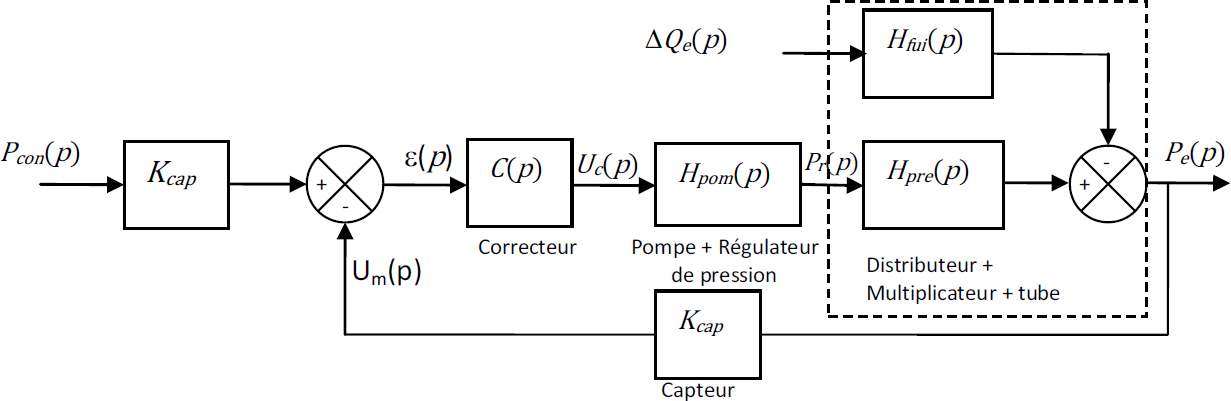
\includegraphics[width=\linewidth]{63_01}
\end{marginfigure}

 
 \begin{tabular}{lp{5cm}}
$P_{\text{con}}(p)$ : & 	pression de consigne d’eau dans le tube (Pa) \\
$P_e(p)$ : & 	pression d’eau dans le tube (Pa) \\
$U_c(p)$ : & 	tension de commande du régulateur de pression (V)\\
$P_r(p)$ : &	pression d’huile régulée (Pa)\\
$\Delta Q_e(p)$ :& 	débit de fuite (\si{m^3s^{-1}})\\
$U_m(p)$ 	:&	tension de mesure du capteur (V)\\
\end{tabular}
 
\textbf{ Hypothèses}
\begin{itemize}
\item L’ensemble de mise sous pression {tube + distributeur + multiplicateur de pression} est défini par les transmittances suivantes : $H_{\text{pre}} (p)=\dfrac{K_m}{1+T_1 p}$	et	$H_{\text{fui}} (p)=\dfrac{K_f}{1+T_1 p}$ avec 	$K_m = 3,24$ ; 	$K_f = \SI{2,55e10}{Pa.m^{-3}.s}$ ; 	$T_1  = \SI{10}{s}$.
\item L’ensemble {pompe+régulateur de pression} est modélisé par la fonction de transfert :
$H_{\text{pom}} (p)=\dfrac{K_{\text{pom}}}{1+T_2 p}$  avec 	$K_{\text{pom}} = \SI{1,234e7}{Pa/V}$; 	$T_2 = \SI{5}{s}$.
\item Le capteur est modélisé par un gain pur :	$K_{\text{cap}} = \SI{2,5e-8}{V/Pa}$.
\end{itemize}
La pression de consigne est de $P_{\text{con}} = \SI{800}{bars}$ et les débits de fuite sont estimés à $\Delta Q_e = \SI{5e-4}{m3/s}$.

 
Le cahier des charges concernant le réglage de la pression de test est le suivant.
\begin{center}
\begin{tabular}{ll}
\hline 
Stabilité :  & marge de phase de 60\degres  \\
  	  &  marge de gain de \SI{12}{dB} \\ \hline
Rapidité :  &  temps d’établissement $t_e < \SI{40}{s}$ (voir remarque ci-dessous) \\ \hline
Précision : & 	erreur statique < 5\% soit pour une consigne de 800 bars : \\
&erreur statique due à la consigne : $\varepsilon_{\text{con}}< 5\%$  \\
& erreur statique due à la perturbation $\varepsilon_{\text{pert}} < \SI{40}{bars}$ \\ \hline
Amortissement :&	pas de dépassement \\ \hline
\end{tabular}
\end{center}

Dans le cas d’un système bouclé convenablement amorti, on pourra utiliser, sans aucune justification, la relation :
$t_e \cdot \omega_{\SI{0}{dB}}=3$ où $\omega_{\SI{0}{dB}}$ désigne la pulsation de coupure à \SI{0}{dB} en boucle ouverte et $t_e$ le temps d’établissement en boucle fermée vis-à-vis d’un échelon de consigne :
\begin{itemize}
\item $t_e = t_m$, temps du 1er maximum si le dépassement est supérieur à \SI{5}{\%},
\item $t_e = t_R$, temps de réponse à \SI{5}{\%} si le dépassement est nul ou inférieur à \SI{5}{\%}.
\end{itemize}

On se propose de corriger le système avec le correcteur défini sur le schéma bloc ci-dessous.

\begin{marginfigure}
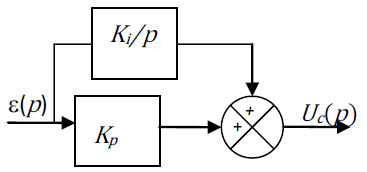
\includegraphics[width=5cm]{63_02}
\end{marginfigure}
\fi

\question{Déterminer la fonction de transfert $C(p)$ de ce correcteur.}
\ifprof
On a $C(p)=\dfrac{K_i}{p}+K_p = \dfrac{K_i+p K_p}{p} = K_i \dfrac{1+p \dfrac{K_p}{K_i}}{p}$.
\else 
\fi


\question{Tracer l’allure de son diagramme de Bode en fonction des coefficients $K_i$ et $K_p$.}
\ifprof

\begin{marginfigure}
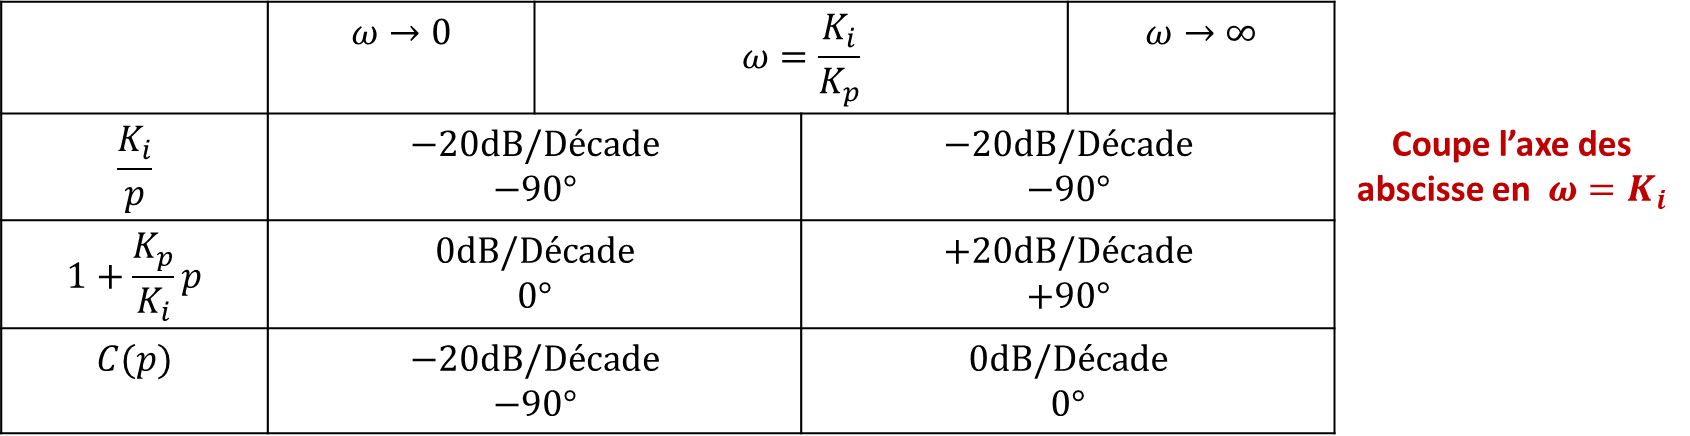
\includegraphics[width=\linewidth]{63_02_cor}
\end{marginfigure}

\begin{marginfigure}
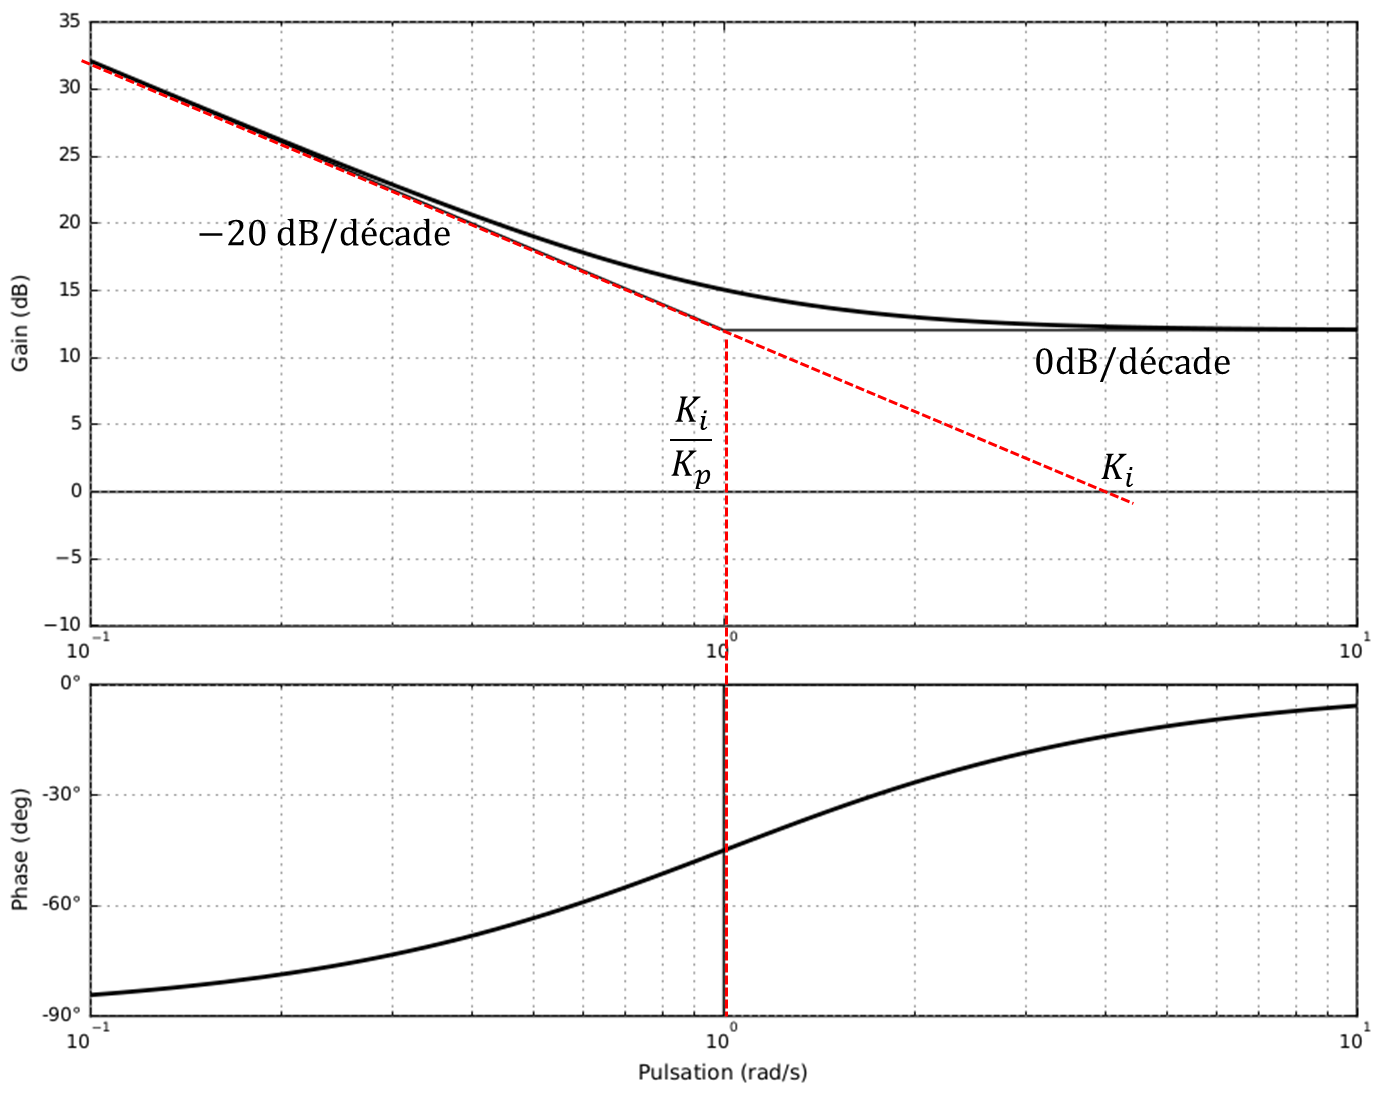
\includegraphics[width=\linewidth]{63_03_cor}
\end{marginfigure}


\else 
\fi


\question{Quelle est l’influence d’un tel correcteur sur la précision et la stabilité ? Justifier.}
\ifprof
Ce correcteur augmente la classe de la FTBO donc augmente la précision. 
Cependant, il réduit la phase. Il faut donc veiller à ce que la pulsation de cassure soit réglée de telle sorte que le système ne soit pas déstabilisé. 
\else 
\fi


\question{Quelle valeur faut-il donner à $\omega_{\SI{0}{dB}}$ pour répondre au critère de rapidité du cahier des charges ?}
\ifprof
D'après la remarque, on a $t_e \omega_{\SI{0}{dB}}=3$ soit $\omega_{\SI{0}{dB}} =3/t_e = \SI{0,075}{rad.s^{-1}}$.
\else 
\fi


\question{Déterminer analytiquement le rapport $T=\dfrac{K_p}{K_i}$ pour obtenir la marge de phase spécifiée dans le cahier des charges.}
\ifprof
Calculons la fonction de transfert en boucle ouverte non corrigée : 
$\indice{F}{BO}=\dfrac{\indice{K}{pom}}{1+T_2 p}\dfrac{\indice{K}{m}}{1+T_1 p} \indice{K}{cap}$.

Le correcteur doit être réglé pour que $\omega_{\SI{0}{dB}} =\SI{0,075}{rad.s^{-1}}$. 

Calculons la marge de phase. 
$\arg\left(\indice{F}{BO}\right)=-\arg\left(1+T_1p\right)-\arg\left(1+T_2p\right) = -\arctan T_1 \omega -\arctan T_2 \omega $
+
On a donc $\arg\left(\indice{F}{BO}(0,075)\right) = -\arctan (10 \times  0,075) -\arctan (5 \times  0,075)=-57\degres$ soit une marge de phase de $-123\degres$.

Pour atteindre une marge de phase de 60\degres, on peut donc baisser la phase de 63\degres.

Calculons $\arg\left(C(j\omega)\right)=-90+\arctan \left(\dfrac{K_p}{K_i}\omega\right)$.

On cherche donc $\dfrac{K_i}{K_p}$ tel que $\arg\left(C(0,075)\right)=-63$
Soit 
$-90+\arctan \left(\dfrac{K_p}{K_i}0,075\right) =-63$
$\Leftrightarrow \arctan \left(\dfrac{K_p}{K_i}0,075\right) =27$
$\Rightarrow  \dfrac{K_p}{K_i}0,075 =0,51$
$\Leftrightarrow  \dfrac{K_p}{K_i}=6,79$.


\else 
\fi


\question{En déduire les valeurs de $K_i$ et $K_p$ qui permettent de régler rapidité et marge de phase.}
\ifprof
Il faut chercher $K_i$ et $K_p$ pour respecter $\omega_{\SI{0}{dB}}$. Recherchons le gain de la boucle ouverte non corrigée pour $\omega_{\SI{0}{dB}}$.

$\indice{G}{dB}\left(\indice{F}{BO}\right)=20\log\left(\indice{K}{pom}\indice{K}{m}\indice{K}{cap}\right)
-20\log\left(\sqrt{1^2+T_1^2\omega^2}\right)-20\log\left(\sqrt{1^2+T_2^2\omega^2}\right)$

On a alors $\indice{G}{dB}\left(\indice{F}{BO}\right)(0,075) = -0,004-1,94-0,57=\SI{2,52}{dB}$.

Il faut donc baisser le gain de \SI{2,52}{dB}
$\indice{G}{dB}\left(C(p)\right)$  
$= 20\log K_i -20\log \omega +20\log\left(\sqrt{1+\left(\dfrac{K_p}{K_i}\right)^2\omega^2}\right) $.

On a alors $\indice{G}{dB}\left(C(0,075)\right) = 20\log K_i +22,5+1 = -2,52$ soit $K_i = 10^{-\dfrac{2,52+1+22,5}{20}  } =0,05$.

Par suite, $K_p = 6,79 \times 0,05 = 0,34$.

(\textbf{A vérifier}).

\else 

On donne les diagrammes de Bode en gain et en phase de la fonction de transfert en boucle ouverte corrigée avec le correcteur Proportionnel Intégral déterminé précédemment. On donne sa réponse temporelle avec et sans débit de fuite pour une pression de consigne d’eau de 800 bars.

\fi



\question{La réponse du système est-elle satisfaisante au regard du cahier des charges ? Justifier.}
\ifprof
\begin{marginfigure}
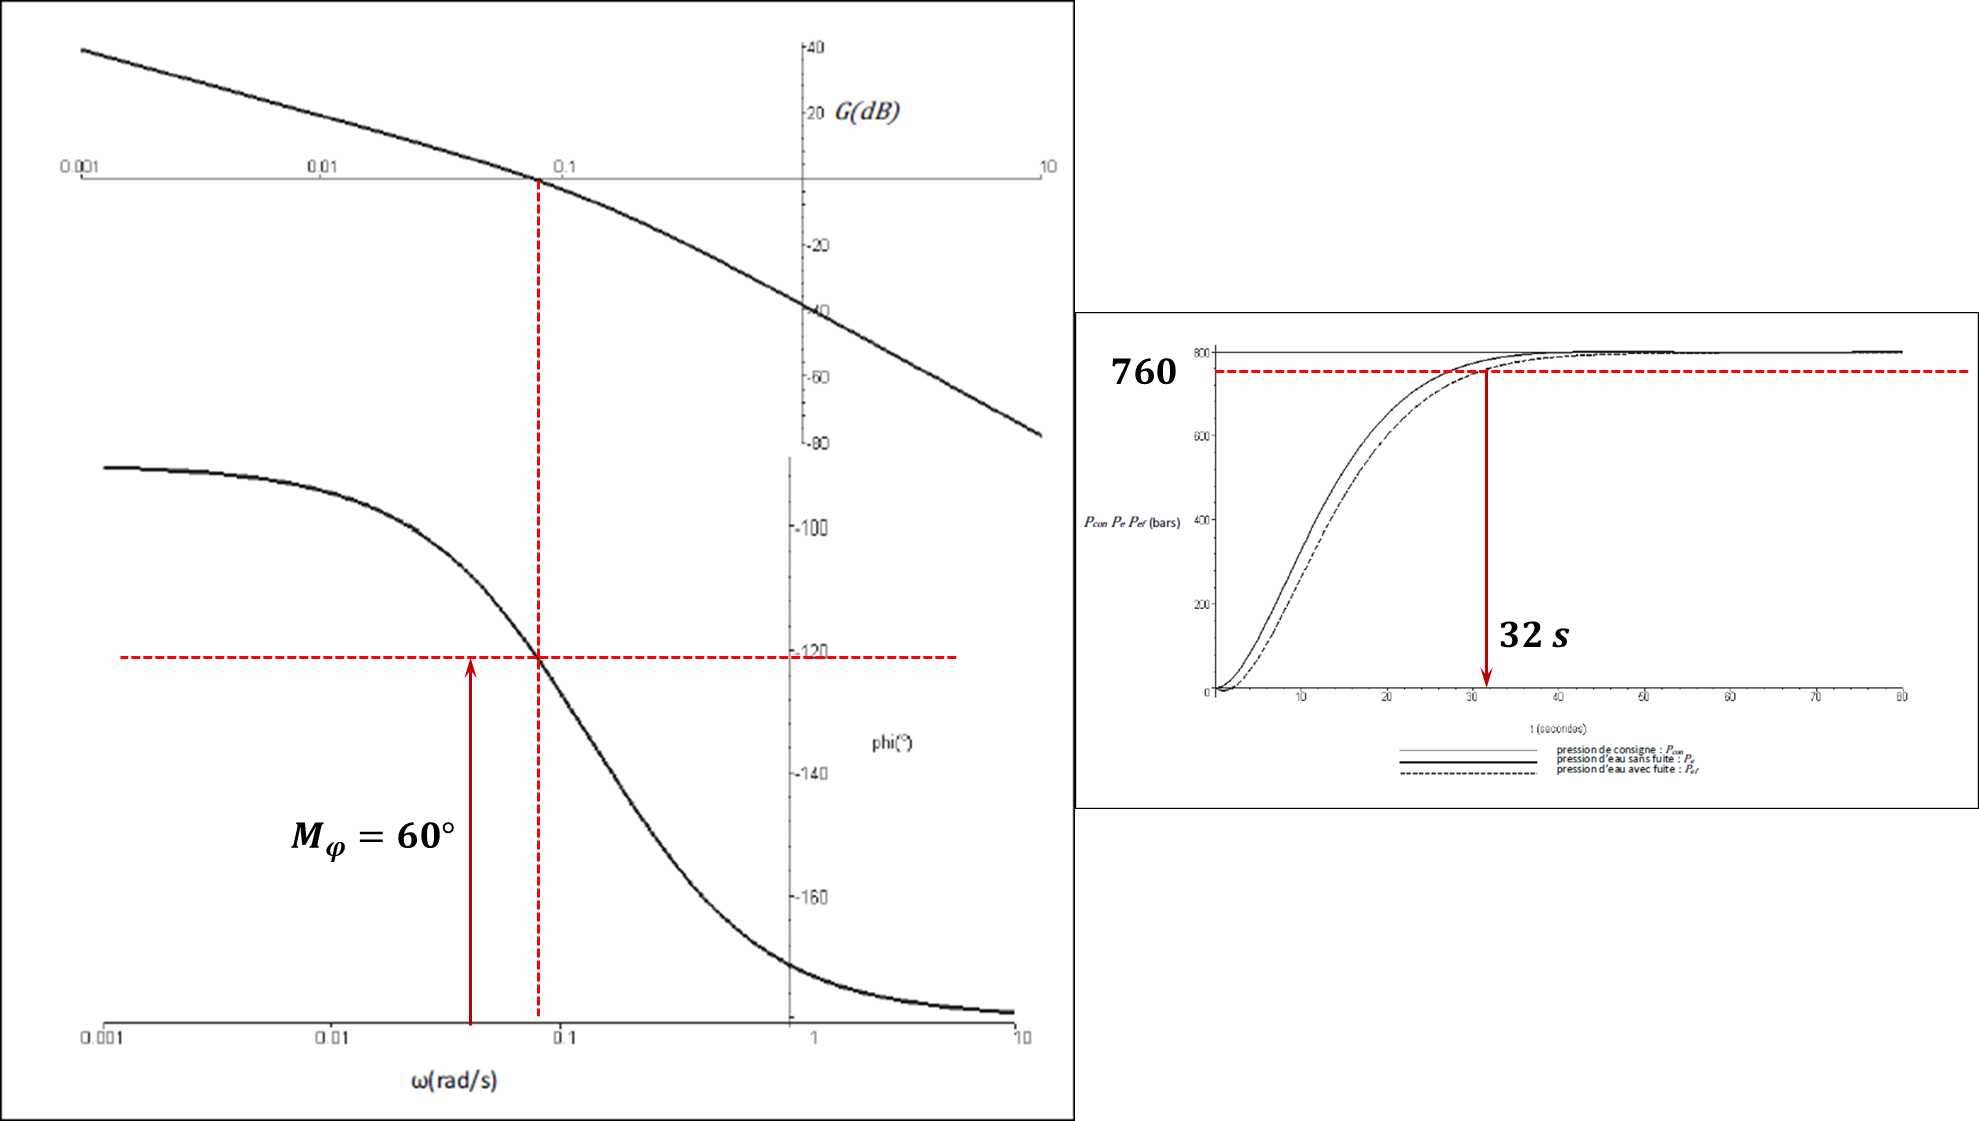
\includegraphics[width=\linewidth]{63_04_cor}
\end{marginfigure}
\begin{itemize}
\item Stabilité : 
\begin{itemize}
\item Marge de phase mesurée :  60\degres \textbf{cdc ok}.
\item Marge de gain mesurée :   infini \textbf{cdc ok}.
\end{itemize}
\item Rapidité : $ t_e = \SI{32}{s} < \SI{40}{s}$ \textbf{cdc ok}.
\item Précision :  écart statique nul \textbf{cdc ok}.
\item Amortissement :  nul \textbf{cdc ok}.
\end{itemize}
\else 
\fi

\ifprof
\else

\begin{marginfigure}
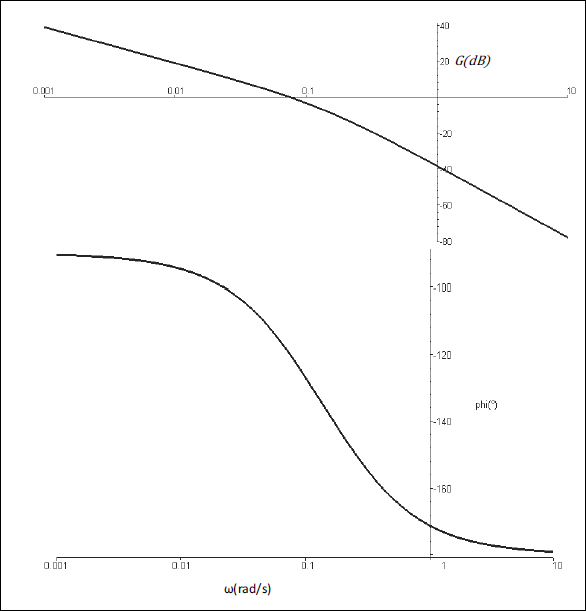
\includegraphics[width=\linewidth]{63_03}
\end{marginfigure}


\begin{marginfigure}
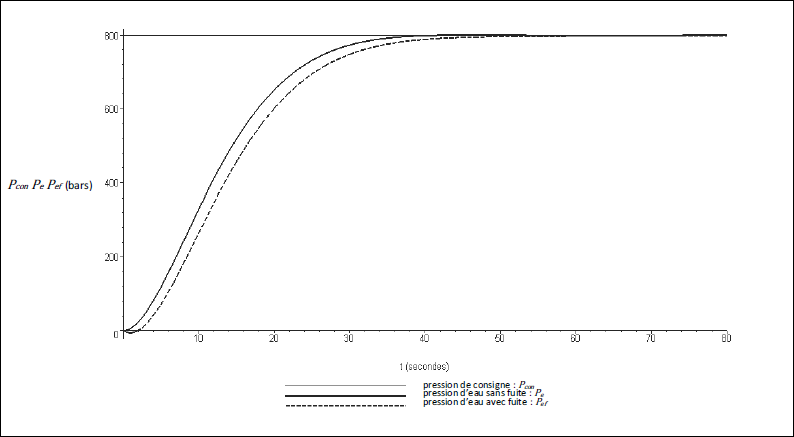
\includegraphics[width=\linewidth]{63_04}
\end{marginfigure}
\fi

\ifprof
\else

\marginnote{\begin{solution} 
\begin{enumerate}
  \item $C(p)= K_i \dfrac{1+p \dfrac{K_p}{K_i}}{p}$.
  \item .
  \item .
  \item $T = 6,79$.
  \item $K_i = 0,05$ et $K_p=0,34$ (à vérifier).
\end{enumerate}
\end{solution}}

\marginnote{Corrigé voir \ref{PERF:02:C2:03:stab:63}.}

\fi 
 
\graphicspath{{\repStyle/png/}{../PERF/PERF-02-Marges/64_EPAS/images/}} 
\normaltrue \difficilefalse \tdifficilefalse
\correctionfalse
%\UPSTIidClasse{11} % 11 sup, 12 spé
%\newcommand{\UPSTIidClasse}{11}

\exer{Exercice d'application $\star$ \label{PERF:02:C2:03:stab:64}}
%% CCP MP 2007
\setcounter{question}{0}\marginnote{\xpComp{PERF}{02}}%\index{Compétence C2-03}\index{Compétence PERF-02}
\index{Compétence C2-03}
\index{Schéma-blocs}
\index{Stabilite}

\ifcorrection
\else
\marginnote{\textbf{Pas de corrigé pour cet exercice.}}
\fi


\ifprof
\else
L'asservissement est donné par le schéma-blocs suivant. $H_{\text{BO}}(p) = \dfrac{4}{p\left( p+3,6\right)}$.  Le retard du système est de \SI{0,2}{s}.
De plus, $C(p)=K_c\dfrac{1+T_c p}{T_c p}$

\begin{marginfigure}
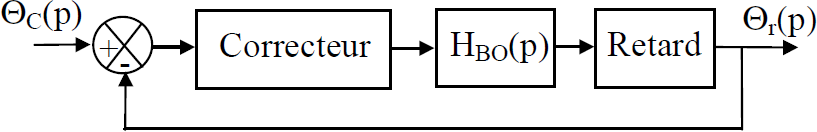
\includegraphics[width=\linewidth]{64_01}
\end{marginfigure}

\fi
 
\question{Tracer le diagramme de Bode asymptotique de $H_{\text{BO}}(p)$ pour des pulsations comprises entre \SI{0,5}{rad.s^{-1}} et \SI{50}{rad.s^{-1}}.}
\ifprof
\else 
\fi

\question{Tracer le diagramme de Bode du retard pour des pulsations comprises entre \SI{0,5}{rad.s^{-1}} et \SI{50}{rad.s^{-1}}.}
\ifprof
\else 
\fi


\ifprof
\else
On donne le diagramme de la FTBO retardée. 

\begin{marginfigure}
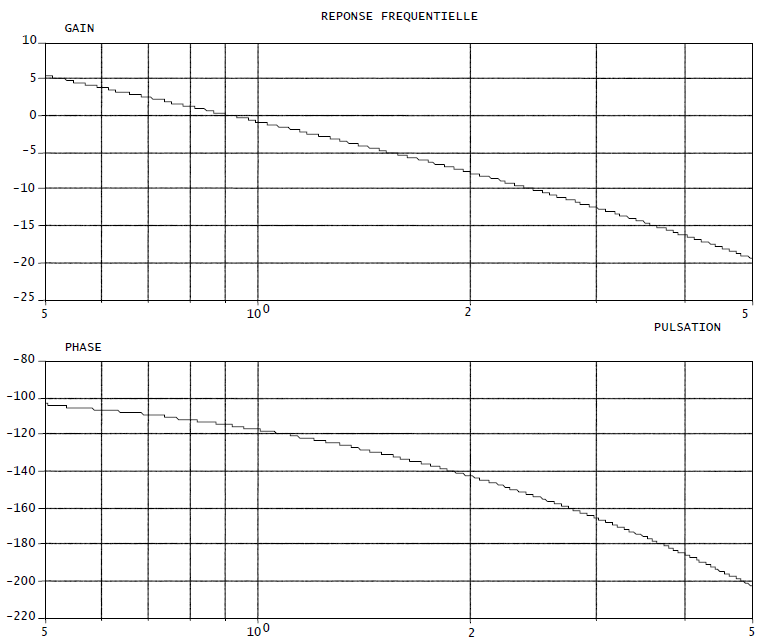
\includegraphics[width=\linewidth]{64_02}
\end{marginfigure}
\fi

\question{Déterminer le gain $K_c$ qui donne une marge de phase de 50\degres.}
\ifprof
\else 
\fi

\question{La constante $T_c$ qui laisse subsister une marge de phase d’environ 45\degres.}
\ifprof
\else 
\fi


\question{Quelle est l’erreur de traînage du système corrigé pour l’entrée en rampe considérée (en négligeant le retard).}
\ifprof
\else 
\fi


\ifprof
\else



\marginnote{Corrigé voir \ref{PERF:02:C2:03:stab:64}.}

\fi 
 
\section{Évaluer la rapidité de la réponse temporelle} 
\section{Évaluer la rapidité à partir de la réponse fréquentielle de la BO} 
\section{Évaluer la précision à partir du TVF} 
\graphicspath{{\repStyle/png/}{../PERF/PERF-05-Precistion-TVF/501_Divers/images/}} 
\normaltrue \difficilefalse \tdifficilefalse
\correctiontrue

%\UPSTIidClasse{11} % 11 sup, 12 spé
%\newcommand{\UPSTIidClasse}{11}

\exer{Valeur finale$\star$ \label{PERF:05:C2:03:501}}
\setcounter{question}{0}\marginnote{\xpComp{PERF}{05}}%\UPSTIcompetence[2]{C2-03}
\index{Compétence C2-03}
\index{Schéma-blocs}
\index{Valeur finale}

\ifcorrection
\else
\marginnote{\textbf{Pas de corrigé pour cet exercice.}}
\fi


\ifprof 
\else
Soit le schéma-blocs suivant.
\begin{marginfigure}
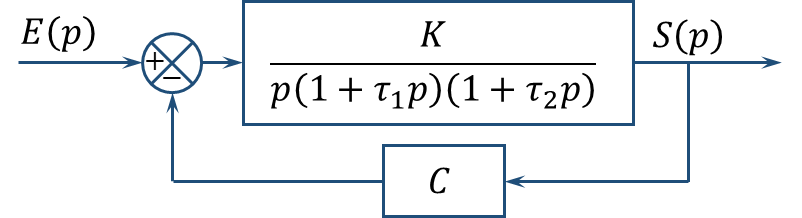
\includegraphics[width=\linewidth]{501_01}
\end{marginfigure}
 \fi
 
\question{Déterminer la valeur finale de $s(t)$ lorsque l'entrée est un échelon d'amplitude $E_0$.}
\ifprof

On a 
$H(p)=\dfrac{\dfrac{K}{p\left(1+\tau_1 p \right)\left(1+\tau_2 p \right)}}{1+\dfrac{CK}{p\left(1+\tau_1 p \right)\left(1+\tau_2 p \right)}}$
$=\dfrac{K}{p\left(1+\tau_1 p \right)\left(1+\tau_2 p \right)+CK}$. 
En conséquence, $S(p)=E(p)\dfrac{K}{p\left(1+\tau_1 p \right)\left(1+\tau_2 p \right)+CK}$.

$s_{\infty}=\lim\limits_{t\to +\infty} s(t)$ $=\lim\limits_{p\to 0} pS(p)$
$=\lim\limits_{p\to 0} pE(p)H(p)$.
Dans le cas où $E(p)$ est un échelon, on a $E(p)=\dfrac{E_0}{p}$ et donc 
$s_{\infty}=\lim\limits_{p\to 0} p\dfrac{E_0}{p}\dfrac{K}{p\left(1+\tau_1 p \right)\left(1+\tau_2 p \right)+CK}=\dfrac{E_0}{C}$.
\else 
\fi

%\question{En déduire la valeur de l'erreur statique.}
%\ifprof
%L'erreur statique est donnée par $\lim\limits_{t\to +\infty} (e(t)-s(t))=E_0 - \dfrac{E_0}{C}$.
%\else
%\fi

\question{Déterminer la valeur finale de $s(t)$ lorsque l'entrée est une rampe de pente $k$.}
\ifprof

On a maintenant $E(p)=\dfrac{k}{p^2}$. 
On a donc et donc 
$s_{\infty}=\lim\limits_{p\to 0} p\dfrac{k}{p^2}\dfrac{K}{p\left(1+\tau_1 p \right)\left(1+\tau_2 p \right)+CK}$ et 
$s_{\infty}=\infty$.

\else 
\fi


%\question{En déduire la valeur de l'erreur de traînage.}
%\ifprof
%$\varepsilon_v = \lim\limits_{t\to +\infty} (e(t)-s(t))$
%$=\lim\limits_{p\to 0} p\left(\dfrac{k}{p^2}-\dfrac{k}{p^2}\dfrac{K}{p\left(1+\tau_1 p \right)\left(1+\tau_2 p \right)+CK}\right)$
%
%$=\lim\limits_{p\to 0} \dfrac{k}{p}\left(1-\dfrac{K}{p\left(1+\tau_1 p \right)\left(1+\tau_2 p \right)+CK}\right)$
%$=\lim\limits_{p\to 0} \dfrac{k}{p}\dfrac{p\left(1+\tau_1 p \right)\left(1+\tau_2 p \right)+CK-K}{p\left(1+\tau_1 p \right)\left(1+\tau_2 p \right)+CK}=+\infty$
%\else
%\fi
%
%\question{Qu'en est-il si $C=1$ ?.}
%\ifprof
%$\varepsilon_v =\lim\limits_{p\to 0} \dfrac{k}{p}\dfrac{p\left(1+\tau_1 p \right)\left(1+\tau_2 p \right)+CK-K}{p\left(1+\tau_1 p \right)\left(1+\tau_2 p \right)+CK}$
%$=\lim\limits_{p\to 0} \dfrac{k}{p}\dfrac{p\left(1+\tau_1 p \right)\left(1+\tau_2 p \right)}{p\left(1+\tau_1 p \right)\left(1+\tau_2 p \right)+K}$
%$=\lim\limits_{p\to 0} k\dfrac{\left(1+\tau_1 p \right)\left(1+\tau_2 p \right)}{p\left(1+\tau_1 p \right)\left(1+\tau_2 p \right)+K} = \dfrac{k}{K}$.


%
%\else
%\fi
%\question{Réaliser le schéma-blocs.}
%\ifprof
%\begin{figure}[H]
%\centering
%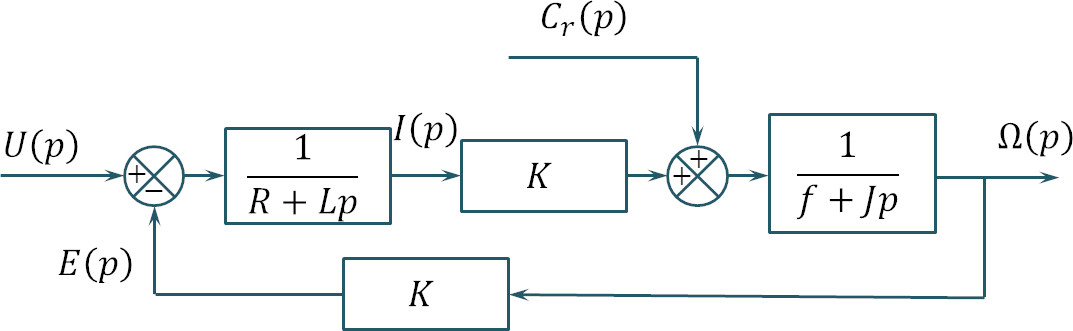
\includegraphics[width=\linewidth]{51_01_c}
%%\caption{Évolution du couple utile en fonction de la vitesse de rotation pour des
%%fréquences de commande de \SI{90}{Hz} à \SI{110}{Hz}. \label{fig_50_04}}
%\end{figure}
%\else
%\fi


 

\ifprof
\else
\marginnote{\begin{solution} 
\begin{enumerate}
    \item $s_{\infty}=\lim\limits_{p\to 0} p\dfrac{E_0}{p}\dfrac{K}{p\left(1+\tau_1 p \right)\left(1+\tau_2 p \right)+CK}=\dfrac{E_0}{C}$.
   % \item $\lim\limits_{t\to +\infty} (e(t)-s(t))=E_0 - \dfrac{E_0}{C}$.
    \item $s_{\infty}=\infty$.
   % \item $\varepsilon_v =\infty$.
%    \item $\varepsilon_v =\dfrac{k}{K}$.
\end{enumerate}
\end{solution}}

\marginnote{Corrigé voir \ref{PERF:05:C2:03:501}.}

\fi 
 
\graphicspath{{\repStyle/png/}{../PERF/PERF-05-Precistion-TVF/509_Divers/images/}} 
\normaltrue \difficilefalse \tdifficilefalse
\correctiontrue

%\UPSTIidClasse{11} % 11 sup, 12 spé
%\newcommand{\UPSTIidClasse}{11}

\exer{Écart$\star$ \label{PERF:05:C2:03:509}}
\setcounter{question}{0}\marginnote{\xpComp{PERF}{05}}%\UPSTIcompetence[2]{C2-03}
\index{Compétence C2-03}
\index{Schéma-blocs}
\index{Valeur finale}
\index{Théorème de la valeur finale}
\index{Erreur}
\ifcorrection
\else
\marginnote{\textbf{Pas de corrigé pour cet exercice.}}
\fi


\ifprof 
\else
Soit le schéma-blocs suivant.
\begin{marginfigure}
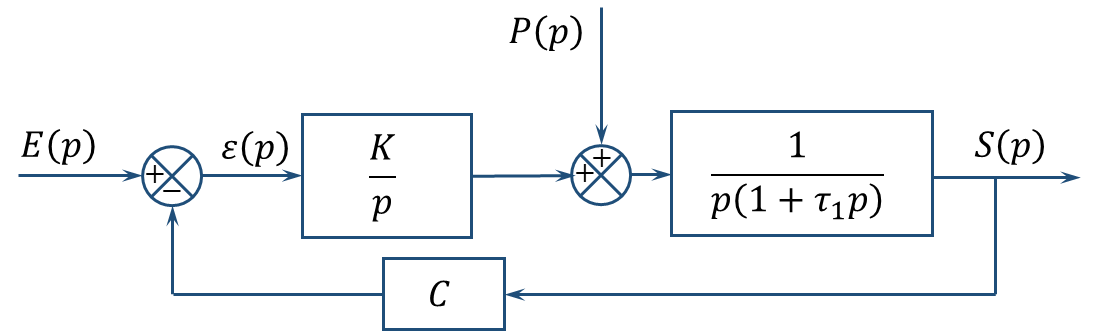
\includegraphics[width=\linewidth]{509_01}
\end{marginfigure}
 \fi
 
\question{Exprimer $\varepsilon(p)$ en fonction de $E(p)$ et $P(p)$.}
\ifprof

On a : 
$\varepsilon(p) = E(p)-C\dfrac{1}{p\left( A+\tau_1 p \right)} \left( \varepsilon(p)\dfrac{K}{p} + P(p)\right)$

$\Leftrightarrow \varepsilon(p) \left(1 +C\dfrac{K}{p^2\left( A+\tau_1 p \right)}\right) = E(p)-C\dfrac{1}{p\left( A+\tau_1 p \right)}  P(p)$

$\Leftrightarrow \varepsilon(p) = E(p)\dfrac{1}{1 +C\dfrac{K}{p^2\left( A+\tau_1 p \right)}}-C\dfrac{1}{p\left( A+\tau_1 p \right)} \dfrac{1}{1 +C\dfrac{K}{p^2\left( A+\tau_1 p \right)}} P(p)$

$\Leftrightarrow \varepsilon(p) = E(p)\dfrac{1}{1 +C\dfrac{K}{p^2\left( A+\tau_1 p \right)}}-\dfrac{C}{p\left( A+\tau_1 p \right) +C\dfrac{K}{p}} P(p)$


\else 
\fi

\question{Évaluer la valeur finale de $\varepsilon(t)$ lorsque $E(p)$ est un échelon d'amplitude $E_0$ et $P(p)$ est un échelon d'amplitude $P_0$.}
\ifprof

On a $\lim\limits_{t\to +\infty} \varepsilon(t) = \lim_{p\to 0} p\varepsilon(p)$.

Dans ces conditons, 
$\varepsilon(p) = E_0\dfrac{1}{p +C\dfrac{K}{p\left( A+\tau_1 p \right)}}-\dfrac{C}{p^2\left( A+\tau_1 p \right) +CK} P_0$.

Au final, $\varepsilon = E_0\dfrac{p}{p +C\dfrac{K}{p\left( A+\tau_1 p \right)}}-\dfrac{Cp}{p^2\left( A+\tau_1 p \right) +CK} P_0$ $=0-0 =0$
\else 
\fi

\question{{Évaluer la valeur finale de $\varepsilon(t)$ lorsque $E(p)$ est un échelon d'amplitude $E_0$ et $P(p)$ est une rampe de pente $P_0$.}
}
\ifprof

Dans ces conditons, 
$\varepsilon(p) = E_0\dfrac{1}{p +C\dfrac{K}{p\left( A+\tau_1 p \right)}}-\dfrac{C}{p^3\left( A+\tau_1 p \right) +CKp} P_0$

et  $\varepsilon = p^2E_0\dfrac{1}{p^2 +C\dfrac{K}{\left( A+\tau_1 p \right)}}-\dfrac{C}{p^2\left( A+\tau_1 p \right) +CK} P_0 = 0 - \dfrac{P_0}{K}=- \dfrac{P_0}{K}$
\else 
\fi

\question{{Évaluer la valeur finale de $\varepsilon(t)$ lorsque $E(p)$ est une rampe de pente $E_0$ et $P(p)$ est un échelon d'amplitude $P_0$.}}
\ifprof

Dans ces conditons, 
$\varepsilon(p) = E_0\dfrac{1}{p^2 +C\dfrac{K}{\left( A+\tau_1 p \right)}}-\dfrac{C}{p^2\left( A+\tau_1 p \right) +CK} P_0$.


On a alors $\varepsilon = pE_0\dfrac{1}{p^2 +C\dfrac{K}{\left( A+\tau_1 p \right)}}-\dfrac{C}{p^2\left( A+\tau_1 p \right) +CK} P_0p = 0$


\else 
\fi

\question{{Évaluer la valeur finale de $\varepsilon(t)$ lorsque $E(p)$ est une rampe de pente $E_0$ et $P(p)$est une rampe de pente  $P_0$.}}
\ifprof

Dans ces conditons, 
$\varepsilon(p) = E_0\dfrac{1}{p^2 +C\dfrac{K}{\left( A+\tau_1 p \right)}}-\dfrac{C}{p^3\left( A+\tau_1 p \right) +CKp} P_0$. 
On a alors
$\varepsilon = E_0 p \dfrac{1}{p^2 +C\dfrac{K}{\left( A+\tau_1 p \right)}}-\dfrac{C}{p^2\left( A+\tau_1 p \right) +CK} p P_0 = -\dfrac{P_0}{K} $.

\else 
\fi




%\question{Réaliser le schéma-blocs.}
%\ifprof
%\begin{figure}[H]
%\centering
%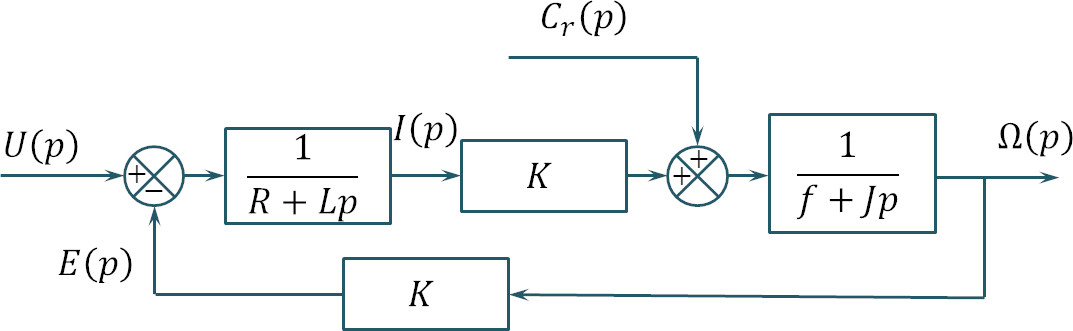
\includegraphics[width=\linewidth]{51_01_c}
%%\caption{Évolution du couple utile en fonction de la vitesse de rotation pour des
%%fréquences de commande de \SI{90}{Hz} à \SI{110}{Hz}. \label{fig_50_04}}
%\end{figure}
%\else
%\fi


 

\ifprof
\else

\marginnote{Corrigé voir \ref{PERF:05:C2:03:509}.}

\fi 
 
\section{Évaluer la précision en utilisant la classe de la BO} 
\graphicspath{{\repStyle/png/}{../PERF/PERF-06-Precision/63_BancHydraulique/images/}} 
\normaltrue \difficilefalse \tdifficilefalse
\correctiontrue
%\UPSTIidClasse{11} % 11 sup, 12 spé
%\newcommand{\UPSTIidClasse}{11}

\exer{Banc hydraulique $\star$ \label{PERF:06:C2:03:prec:63}}
%% CCP MP 2010
\setcounter{question}{0}\marginnote{\xpComp{PERF}{06}}%\UPSTIcompetence[2]{C2-03}
\index{Compétence C2-03}
\index{Schéma-blocs}
\index{Précision}

\ifcorrection
\else
\marginnote{\textbf{Pas de corrigé pour cet exercice.}}
\fi

\ifprof
\else 

Pour limiter l’erreur statique due aux fuites, on envisage d’asservir la pression d’eau dans le tube. 
%L’objectif est ici de proposer un réglage du correcteur pour répondre aux critères du cahier des charges.
La pression d’eau à l’intérieur du tube est mesurée par un capteur de pression. 

\begin{marginfigure}
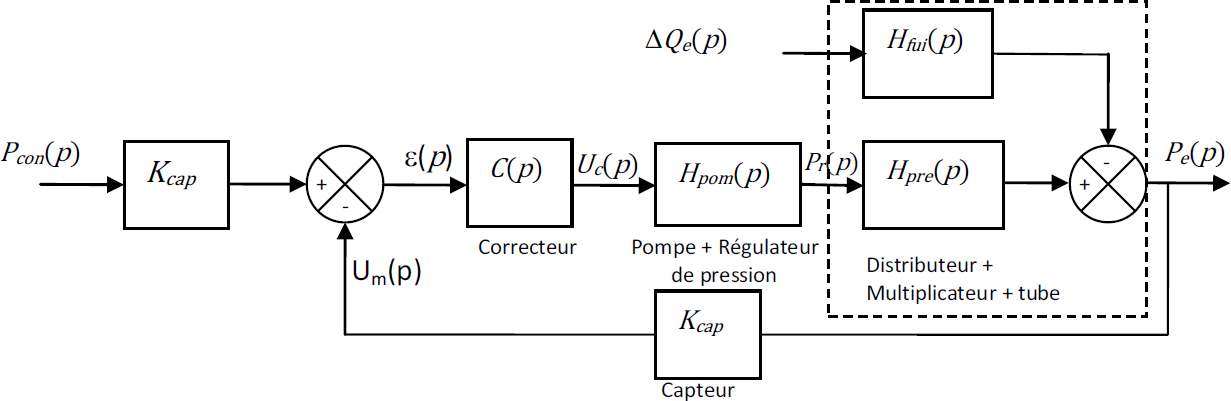
\includegraphics[width=\linewidth]{63_01}
\end{marginfigure}

 
 \begin{tabular}{ll}
$P_{\text{con}}(p)$ : & 	pression de consigne d’eau dans le tube (Pa) \\
$P_e(p)$ : & 	pression d’eau dans le tube (Pa) \\
$U_c(p)$ : & 	tension de commande du régulateur de pression (V)\\
$P_r(p)$ : &	pression d’huile régulée (Pa)\\
$\Delta Q_e(p)$ :& 	débit de fuite (\si{m^3s^{-1}})\\
$U_m(p)$ 	:&	tension de mesure du capteur (V)\\
\end{tabular}
 
 Hypothèses :
\begin{itemize}
\item L’ensemble de mise sous pression {tube + distributeur + multiplicateur de pression} est défini par les transmittances suivantes : $H_{\text{pre}} (p)=\dfrac{K_m}{1+T_1 p}$	et	$H_{\text{fui}} (p)=\dfrac{K_f}{1+T_1 p}$ avec 	$K_m = 3,24$ ; 	$K_f = \SI{2,55e10}{Pa.m^{-3}.s}$ ; 	$T_1  = \SI{10}{s}$.
\item L’ensemble {pompe+régulateur de pression} est modélisé par la fonction de transfert :
$H_{\text{pom}} (p)=\dfrac{K_{\text{pom}}}{1+T_2 p}$  avec 	$K_{\text{pom}} = \SI{1,234e7}{Pa/V}$; 	$T_2 = \SI{5}{s}$.
\item Le capteur est modélisé par un gain pur :	$K_{\text{cap}} = \SI{2,5e-8}{V/Pa}$.
\end{itemize}
La pression de consigne est de $P_{\text{con}} = \SI{800}{bars}$ et les débits de fuite sont estimés à $\Delta Q_e = \SI{5e-4}{m3/s}$.

 
Le cahier des charges concernant le réglage de la pression de test est le suivant.
\begin{center}
\begin{tabular}{lp{8cm}}
\hline 
Stabilité :  & marge de phase de 60\degres  \\
  	  &  marge de gain de \SI{12}{dB} \\ \hline
Rapidité :  &  temps d’établissement te < 40 s \\ \hline
Précision : & 	erreur statique < 5\% soit pour une consigne de 800 bars : \\
&erreur statique due à la consigne : $\varepsilon_{\text{con}}< 5\%$  \\
& erreur statique due à la perturbation $\varepsilon_{\text{pert}} < \SI{40}{bars}$ \\ \hline
Amortissement :&	pas de dépassement \\ \hline
\end{tabular}
\end{center}

Dans le cas d’un système bouclé convenablement amorti, on pourra utiliser, sans aucune justification, la relation :
$t_e \cdot \omega_{\SI{0}{dB}}=3$ où $\omega_{\SI{0}{dB}}$ désigne la pulsation de coupure à \SI{0}{dB} en boucle ouverte et $t_e$ le temps d’établissement en boucle fermée vis-à-vis d’un échelon de consigne :
\begin{itemize}
\item $t_e = t_m$, temps du 1er maximum si le dépassement est supérieur à \SI{5}{\%},
\item $t_e = t_R$, temps de réponse à \SI{5}{\%} si le dépassement est nul ou inférieur à \SI{5}{\%}.
\end{itemize}
On envisage tout d’abord un correcteur de type proportionnel : $C(p)=K_p$. 
\fi

\question{Déterminer, en fonction de $K_p$ ,  $\varepsilon_{\text{con}}$ définie comme l’erreur statique pour une entrée consigne $P_{\text{con}}$ de type échelon, dans le cas où le débit de fuite est nul.}
\ifprof

Le débit de fuite est nul; donc $\Delta Q_e(p)=0$.

\textbf{Cas 1 : cours sur la précision connu \textit{-- Attention à avoir le même type d'entrée/sortie}}

La FTBO est de classe nulle ($C(p)$ est un gain, $H_{\text{pom}} (p)$ et $H_{\text{pre}} (p)$ de classe 0). Le gain de la Boucle ouverte est $K_{\text{BO}}=K_p K_m K_{\text{pom}}K_{\text{cap}}$.


Si l'entrée est un échelon d'amplitude $P_0$, l'écart statique est donc donné par 
$\varepsilon_S = \dfrac{P_0}{1+K_{\text{BO}}}= \dfrac{P_0}{1+K_p K_m K_{\text{pom}}K_{\text{cap}}}$.



\textbf{Cas 2 : cours sur la précision peu connu -- À savoir faire, mais on perd un peu de temps... \textit{-- Attention à avoir le même type d'entrée/sortie}}
Si on connait quand même un petit peu son cours, on a 
$\varepsilon(p)
=
\dfrac{P_{\text{con}}(p)}%
{1+K_P \dfrac{K_{\text{pom}}}{1+T_2 p} \dfrac{K_m}{1+T_1 p} K_{\text{cap}}}$.

On a alors,
$\varepsilon_s = \lim\limits_{p\to 0} p 
\dfrac{\dfrac{P_0}{p}}%
{1+K_P \dfrac{K_{\text{pom}}}{1+T_2 p} \dfrac{K_m}{1+T_1 p} K_{\text{cap}}}$
$=
\dfrac{P_0}%
{1+K_P K_{\text{pom}}K_m K_{\text{cap}}}
$

\textbf{Cas 3 : cours sur la précision pas connu -- À savoir faire, mais on perd beaucoup peu de temps...}

En utilisant la formule de Black, on a $P_e(p) 
= P_{\text{con}}(p) K_{\text{cap}} 
\dfrac{K_P \dfrac{K_{\text{pom}}}{1+T_2 p} \dfrac{K_m}{1+T_1 p} }%
{1+K_P \dfrac{K_{\text{pom}}}{1+T_2 p} \dfrac{K_m}{1+T_1 p} K_{\text{cap}}}$

$= P_{\text{con}}(p) K_{\text{cap}}(p) 
\dfrac{K_P K_{\text{pom}}K_m }%
{\left(1+T_2 p\right)\left(1+T_1 p\right)+K_P K_{\text{pom}} K_m K_{\text{cap}}}$

En passant à la valeur finale avec une entrée échelon, on a 
$\lim\limits_{t\to +\infty}P_e(t)$ $ =  P_{0} K_{\text{cap}} 
\dfrac{K_P K_{\text{pom}}K_m }%
{1+K_P K_{\text{pom}} K_m K_{\text{cap}}}$

L'écart statique est donc donné par
$
\varepsilon_S = P_0 - P_{0} 
\dfrac{K_P K_{\text{pom}}K_m K_{\text{cap}} }%
{1+K_P K_{\text{pom}} K_m K_{\text{cap}}}$
$= P_0
\dfrac{1+K_P K_{\text{pom}} K_m K_{\text{cap}} - K_P K_{\text{pom}}K_m K_{\text{cap}} }{1+K_P K_{\text{pom}} K_m K_{\text{cap}}}
$

$= 
\dfrac{P_0}{1+K_P K_{\text{pom}} K_m K_{\text{cap}}}$

\else 
\fi

\question{Proposer un réglage de $K_p$ pour limiter $\varepsilon_{\text{con}}$ à la valeur spécifiée dans le cahier des charges.}
\ifprof
On souhaite que l'écart statique soit inférieure à 5\% soit 0,05 pour une entrée unitaire. 

On cherche donc $K_P$ tel que 
$\dfrac{1}{1+K_P K_{\text{pom}} K_m K_{\text{cap}}}<0,05 $
$ \Leftrightarrow 1<0,05\left(1+K_P K_{\text{pom}} K_m K_{\text{cap}}\right)$

$ \Leftrightarrow \dfrac{1 - 0,05}{0,05 K_{\text{pom}} K_m K_{\text{cap}}}<K_P $

Soit $ K_P > \dfrac{1 - 0,05}{0,05 \times 1,234 \times 10^7\times 3,24 \times  2,5 \times 10^{-8}}  \Rightarrow K_P > 19$.
\else 
\fi

\question{Dans le cas où la consigne de pression est nulle,  déterminer en fonction de $K_p$ la fonction de transfert en régulation définie par : $H_{\text{pert}}(p)=\dfrac{P_e (p)}{\Delta Q_e (p)}$. En déduire, en fonction de $K_p$,  $\varepsilon_{\text{pert}}$  définie comme l’erreur statique pour une perturbation $\Delta Q_e$ de type échelon, dans le cas où la consigne de pression est nulle.}
\ifprof
Dans ce cas il n'y a pas d'intégrateur avant la perturbation échelon. Il faut savoir faire le calcul.

On peut utiliser la << lecture directe >> :
$P_e(p)= P_r(p)\indice{H}{pre} - \Delta Q_e(p) \indice{H}{fui}(p)$

$= \indice{H}{pre}(p)\indice{H}{pom}(p) C(p) \varepsilon(p)- \Delta Q_e(p) \indice{H}{fui}(p)$

$= -\indice{H}{pre}(p)\indice{H}{pom}(p) C(p) \indice{K}{cap} P_e(p)- \Delta Q_e(p) \indice{H}{fui}(p)$.

$\Leftrightarrow P_e(p) \left(1+\indice{H}{pre}(p)\indice{H}{pom}(p) C(p) \indice{K}{cap} \right)
=- \Delta Q_e(p) \indice{H}{fui}(p)$

$\Leftrightarrow \dfrac{P_e(p)}{\Delta Q_e(p)} 
=-  \dfrac{\indice{H}{fui}(p)}{1+\indice{H}{pre}(p)\indice{H}{pom}(p) C(p) \indice{K}{cap}}$


Calculons $\indice{\varepsilon}{pert}(p) = -  \dfrac{\indice{H}{fui}(p)}{1+\indice{H}{pre}(p)\indice{H}{pom}(p) C(p) \indice{K}{cap}} \Delta Q_e(p) \indice{K}{cap}$.

On a alors $\indice{\varepsilon}{pert}= \tvf{\varepsilon}$ 
$= \lim\limits_{p\to 0} - p\times  \dfrac{\indice{H}{fui}(p)}{1+\indice{H}{pre}(p)\indice{H}{pom}(p) C(p) \indice{K}{cap}} \dfrac{\Delta Q_0}{p} \indice{K}{cap}$

$= - \dfrac{K_f\Delta Q_0 \indice{K}{cap}}{1+K_m\indice{K}{pom} K_P \indice{K}{cap}} $

\else 
\fi

\question{Proposer un réglage de $K_p$ pour limiter $\varepsilon_{\text{pert}}$ à la valeur spécifiée au cahier des charges.}
\ifprof
Pour $\Delta Q_e = \SI{5e-4}{m^3.s^{-1}}$, il faut $\indice{\varepsilon}{pert}<40\times 10^5$ (Pa) soit

$\dfrac{K_f\Delta Q_0 \indice{K}{cap} }{1+K_m\indice{K}{pom} K_P \indice{K}{cap}}  < 40\times 10^5$
$\Rightarrow  K_f\Delta Q_0 \indice{K}{cap}  < 40\times 10^5\left(1+K_m\indice{K}{pom} K_P \indice{K}{cap}\right)$
$\Rightarrow \dfrac{K_f\Delta Q_0 \indice{K}{cap}  -40\times 10^5}{40\times 10^5 K_m\indice{K}{pom} \indice{K}{cap} }< K_P $
$\Rightarrow K_P > -1$
\else 
\fi

\question{Proposer un réglage de $K_p$ pour vérifier le critère d’amortissement. Conclure quant au choix d’un correcteur proportionnel.}
\ifprof
Je vous laisse faire le calcul... Il faut savoir le faire le plus vite possible.
Il faut d'abord calculer la FTBF, la mettre sous forme canonique, déterminer 
$\indice{\xi}{BF}=\dfrac{T_1+T_2}{2\sqrt{T_1T\left( 1+K_P K_M \indice{K}{Pom}\indice{K}{Cap}\right)}}$ puis
determiner $K_P$ tel que $\indice{\xi}{BF}=1$.

\else 
\fi
 

\ifprof
\else
\begin{solution}
\begin{enumerate}
  \item $\varepsilon_{\text{con \%}} = \dfrac{1}{1+K_PK_m K_{\text{pom}} K_{\text{cap}} }$;
  \item $K_P > 19$;
  \item $\varepsilon_{\text{pert}} = \Delta Q_e \dfrac{K_f}{1+K_{\text{cap}}K_PK_mK_{\text{pom}}}$;
  \item $K_P > -1$.% $K_P > 2,19$.
  \item $K_P < 0,125$. Il est impossible de vérifier les trois conditions avec un correcteur proportionnel.
\end{enumerate}
\end{solution}

\marginnote{Corrigé voir \ref{PERF:06:C2:03:prec:63}.}

\fi 
 
\graphicspath{{\repStyle/png/}{../PERF/PERF-06-Precision/64_EPAS/images/}} 
\normaltrue \difficilefalse \tdifficilefalse
\correctionfalse
%\UPSTIidClasse{11} % 11 sup, 12 spé
%\newcommand{\UPSTIidClasse}{11}

\exer{Exercice $\star$ \label{PERF:06:C2:03:prec:64}}
%% CCP MP 2007
\setcounter{question}{0}\marginnote{\xpComp{PERF}{06}}%\UPSTIcompetence[2]{C2-03}
\index{Compétence C2-03}
\index{Schéma-blocs}
\index{Précision}

\ifcorrection
\else
\marginnote{\textbf{Pas de corrigé pour cet exercice.}}
\fi


\ifprof
\else
On donne le système suivant dont la la FTBF est donnée par 
$G(p)=\dfrac{\Theta_S(p)}{\Theta_C(p)}=\dfrac{3,24}{p^2+3,24 p+3,24}$. Le retard du système est de \SI{0,2}{s}.

L'asservissement est donné par le schéma-blocs suivant.

\begin{marginfigure}
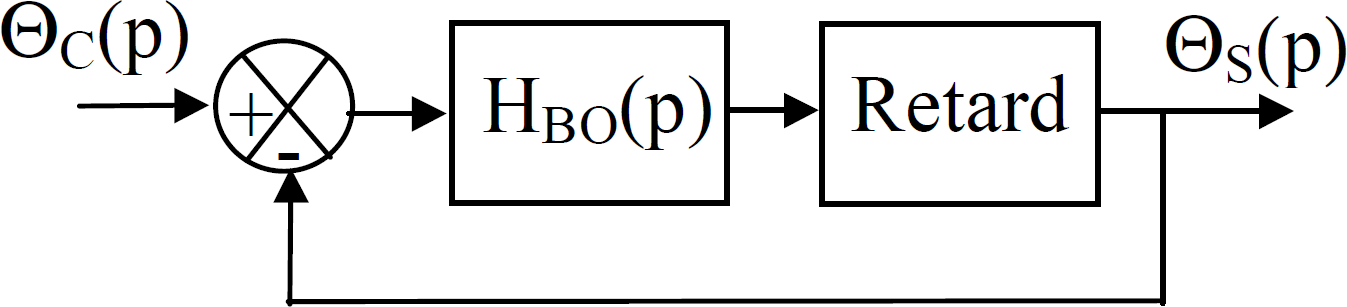
\includegraphics[width=\linewidth]{64_01}
\end{marginfigure}

\fi

 
\question{En considérant le retard nul, déterminer l'écart statique.}
\ifprof
\else 
\fi

\question{En considérant le retard nul, déterminer l'écart statique, déterminer l'expression de la boucle ouverte $H_{\text{BO}}(p)$.}
\ifprof
\else 
\fi
 
\question{Déterminer l'expression de $G_r(p)$, transmittance en boucle fermée du système avec retard de \SI{0,2}{s}.}
\ifprof
\else 
\fi
Le système est soumise à une rampe de \SI{0,1}{rad.s^{-1}}.
 
\question{Donner la valeur de l’erreur de traînage correspondant à cette entrée, en
négligeant le retard.}
\ifprof
\else 
\fi
 
\question{Donner la valeur de l'écart statique du système avec retard.}
\ifprof
\else 
\fi
 
\question{Donner la valeur de l'erreur de traînage du système avec retard.}
\ifprof
\else 
\fi

\ifprof
\else

\noindent\footnotesize
% \fbox{\parbox{.9\linewidth}{
% Éléments de corrigé : 
% \begin{enumerate}
  % \item $\varepsilon_{\text{con \%}} = \dfrac{1}{1+K_PK_m K_{\text{pom}} K_{\text{cap}} }$;
  % \item $K_P > 19$;
  % \item $\varepsilon_{\text{pert}} = \Delta Q_e \dfrac{K_f}{1+K_{\text{cap}}K_PK_mK_{\text{pom}}}$;
  % \item $K_P > 2,19$.
  % \item $K_P < 0,125$. Il est impossible de vérifier les trois conditions avec un correcteur proportionnel.
% \end{enumerate}}}
\normalsize


\marginnote{Corrigé voir \ref{PERF:06:C2:03:prec:64}.}

\fi 
 
\graphicspath{{\repStyle/png/}{../PERF/PERF-06-Precision/73_Bassin/images/}} 
\normaltrue \difficilefalse \tdifficilefalse
\correctionfalse
%\UPSTIidClasse{11} % 11 sup, 12 spé
%\newcommand{\UPSTIidClasse}{11}

\exer{Exercice $\star$ \label{PERF:06:C2:03:prec:73}}
%% CCP MP 2007
\setcounter{question}{0}\marginnote{\xpComp{PERF}{06}}%\UPSTIcompetence[2]{C2-03}
\index{Compétence C2-03}
\index{Schéma-blocs}
\index{Précision}

\ifcorrection
\else
\marginnote{\textbf{Pas de corrigé pour cet exercice.}}
\fi


\ifprof
\else
L'asservissement de vitesse est à présent modélisé par le schéma-blocs de la figure suivante à retour unitaire. Cet asservissement n’est valable que pour les petites variations de vitesse. $H(p)$ correspond à la fonction de transfert en boucle ouverte naturelle (non corrigée), $C(p)$ est le correcteur.

\begin{marginfigure}
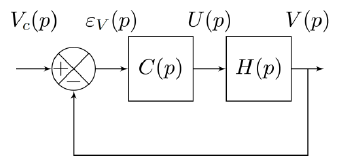
\includegraphics[width=\linewidth]{73_01}
\end{marginfigure}

 $H(p)=\dfrac{K_N}{(1+T_m p)(1+T_e p)}$ avec $K_N = \SI{20}{ms.^{-1}V^{-1}}$, $T_m = \SI{5}{s}$, $T_e = \SI{0,5}{s}$.
 
 \begin{obj}
\begin{itemize}
\item  Exigence 1.2 : Garantir un déplacement du chariot de vitesse : 
\begin{itemize}
\item  1.2.3 Précision :
\begin{itemize}
\item Erreur statique pour une entrée $v_c(t)=V_0 u(t)$ avec $V_0 = \SI{8}{m.s^{-1}}$ : $E_S = \SI{0}{m.s^{-1}}$.
\item Erreur de trainage pour une entrée $v_c(t)=\gamma_0 t  u(t)$ avec $\gamma_0 = \SI{1,6}{m.s^{-2}}$ : $E_T \leq   \SI{0,16}{m.s^{-1}}$.
\end{itemize}
\end{itemize}
\end{itemize}
 \end{obj}
 Le concepteur choisit un correcteur Proportionnel Intégral : $C_1(p)=\dfrac{C}{T_i p} \left(1+T_i p\right)$ avec $T_i = T_m$.
 
\fi
 
 
\question{Déterminer les expressions littérales de l'erreur statique $E_S$ (consigne : échelon d'amplitude $V_0$) et de l'erreur de trainage $E_T$ (consigne : rampe de pente $\gamma_0$) de cet asservissement corrigé avec $C_1(p)$ en fonction de la consigne, du gain $K_N$ et des paramètres du correcteur et $C$  et $T_m$.}
\ifprof
\else 
\fi

\question{ En déduire la condition (notée $C_{\varepsilon}$) sur le gain $C$ du correcteur permettant de satisfaire l’exigence 1.2.3 du cahier des charges.}
\ifprof
\else 
\fi

On choisit finalement un correcteur PID : $C_2(p)=C\left(1+\dfrac{1}{T_i p}+T_d p \right)$ avec $T_i = 2 T_e$ et $T_d = \dfrac{T_e}{2}$.

\question{Montrer qu'on peut mettre ce correcteur sous la forme  $C_2(p)= \dfrac{K}{p}\left(1+Tp\right)^2$ et donner les expressions de $K$  et de $T$ en fonction de $C$ et $T_e$.}
\ifprof
\else 
\fi


\question{Donner l'expression de la fonction de transfert en boucle ouverte du système corrigé.}
\ifprof
\else 
\fi

\question{Déterminer les expressions littérales de l'erreur statique $E_S$ (consigne : échelon d'amplitude $V_0$) et de l'erreur de traînage $E_T$ (consigne : rampe de pente $\gamma_0$) de cet asservissement corrigé.}
\ifprof
\else 
\fi

\question{ En déduire la condition sur la valeur du gain $K$ du correcteur permettant de satisfaire l’exigence 1.2.3 du cahier des charges.}
\ifprof
\else 
\fi

\ifprof
\else


\marginnote{Corrigé voir \ref{PERF:06:C2:03:prec:73}.}

\fi 
 

\end{document}
